% =====================================================================================
% Online supplement of the EJOR manuscript (compiled separately: supplement.pdf).
% Every table here is generated by gerar_tabelas.py / gerar_suplemento.py from the raw per-run files;
% numbering S1, S2, ... follows the order of the \input lines (mirrored in suptab.tex, which the manuscript
% reads to cite "Table S<k>").
% =====================================================================================
\documentclass[11pt]{article}
\usepackage[margin=2.5cm]{geometry}
\usepackage{amsmath,amssymb}
\usepackage{booktabs}
\usepackage{array}
\usepackage{graphicx}
\usepackage{adjustbox}
\usepackage{longtable}
\usepackage{algorithm}
\usepackage{algpseudocode}
\renewcommand{\thealgorithm}{S\arabic{algorithm}}
\usepackage{xcolor}
\usepackage[authoryear]{natbib}
\usepackage[colorlinks=true,linkcolor=blue!50!black,citecolor=blue!50!black,urlcolor=blue!50!black]{hyperref}
% GERADO por gerar_tabelas.py -- NAO EDITAR A MAO
\makeatletter
\expandafter\gdef\csname num@compl_2opt\endcsname{17.6}
\expandafter\gdef\csname num@compl_algum_barato\endcsname{25.8}
\expandafter\gdef\csname num@compl_algum_caro\endcsname{72.9}
\expandafter\gdef\csname num@compl_cross\endcsname{32.3}
\expandafter\gdef\csname num@compl_n\endcsname{1\,776}
\expandafter\gdef\csname num@compl_oropt\endcsname{11.1}
\expandafter\gdef\csname num@compl_so_baratos\endcsname{2.7}
\expandafter\gdef\csname num@compl_so_caros\endcsname{49.8}
\expandafter\gdef\csname num@compl_swapintra\endcsname{0.0}
\expandafter\gdef\csname num@compl_swapstar\endcsname{63.8}
\expandafter\gdef\csname num@diag_n\endcsname{740}
\expandafter\gdef\csname num@diag_otimo\endcsname{54}
\expandafter\gdef\csname num@diag_otimo_max\endcsname{62}
\expandafter\gdef\csname num@diag_otimo_min\endcsname{36}
\expandafter\gdef\csname num@diag_ultima\endcsname{82}
\expandafter\gdef\csname num@eff_0\endcsname{0.364}
\expandafter\gdef\csname num@eff_1\endcsname{0.219}
\expandafter\gdef\csname num@eff_2\endcsname{0.019}
\expandafter\gdef\csname num@eff_3\endcsname{0.111}
\expandafter\gdef\csname num@eff_4\endcsname{0.065}
\expandafter\gdef\csname num@eff_5\endcsname{0.192}
\expandafter\gdef\csname num@eff_6\endcsname{0.088}
\expandafter\gdef\csname num@eff_7\endcsname{0.166}
\expandafter\gdef\csname num@eff_8\endcsname{0.013}
\expandafter\gdef\csname num@eff_9\endcsname{0.009}
\expandafter\gdef\csname num@eff_best\endcsname{2-Opt}
\expandafter\gdef\csname num@eff_cost_0\endcsname{1.1}
\expandafter\gdef\csname num@eff_cost_1\endcsname{1.9}
\expandafter\gdef\csname num@eff_cost_2\endcsname{18.9}
\expandafter\gdef\csname num@eff_cost_3\endcsname{4.5}
\expandafter\gdef\csname num@eff_cost_4\endcsname{3.8}
\expandafter\gdef\csname num@eff_cost_5\endcsname{1.8}
\expandafter\gdef\csname num@eff_cost_6\endcsname{5.2}
\expandafter\gdef\csname num@eff_cost_7\endcsname{2.0}
\expandafter\gdef\csname num@eff_cost_8\endcsname{24.7}
\expandafter\gdef\csname num@eff_cost_9\endcsname{70.9}
\expandafter\gdef\csname num@eff_cost_ratio\endcsname{63}
\expandafter\gdef\csname num@eff_ratio\endcsname{42}
\expandafter\gdef\csname num@eff_suc_0\endcsname{37.3}
\expandafter\gdef\csname num@eff_suc_1\endcsname{38.7}
\expandafter\gdef\csname num@eff_suc_2\endcsname{24.4}
\expandafter\gdef\csname num@eff_suc_3\endcsname{33.4}
\expandafter\gdef\csname num@eff_suc_4\endcsname{10.6}
\expandafter\gdef\csname num@eff_suc_5\endcsname{24.3}
\expandafter\gdef\csname num@eff_suc_6\endcsname{37.2}
\expandafter\gdef\csname num@eff_suc_7\endcsname{30.3}
\expandafter\gdef\csname num@eff_suc_8\endcsname{21.5}
\expandafter\gdef\csname num@eff_suc_9\endcsname{40.0}
\expandafter\gdef\csname num@eff_worst\endcsname{SWAP*}
\expandafter\gdef\csname num@eq_005\endcsname{0}
\expandafter\gdef\csname num@eq_010\endcsname{18}
\expandafter\gdef\csname num@eq_015\endcsname{31}
\expandafter\gdef\csname num@eq_020\endcsname{40}
\expandafter\gdef\csname num@eq_best_lo90\endcsname{0.15}
\expandafter\gdef\csname num@eq_n\endcsname{58}
\expandafter\gdef\csname num@eq_n_aos\endcsname{50}
\expandafter\gdef\csname num@eq_shapiro\endcsname{56}
\expandafter\gdef\csname num@g_acc_abs\endcsname{0.09--0.21}
\expandafter\gdef\csname num@g_gvns_r1\endcsname{0.5}
\expandafter\gdef\csname num@g_ord_best_abs\endcsname{0.34--0.38}
\expandafter\gdef\csname num@g_ord_r1\endcsname{0.3--0.5}
\expandafter\gdef\csname num@g_ord_shaken_abs\endcsname{0.30--0.48}
\expandafter\gdef\csname num@g_pool_r1\endcsname{0.5}
\expandafter\gdef\csname num@g_s3_vsfoc_abs\endcsname{0.17--0.30}
\expandafter\gdef\csname num@g_s5_A1\endcsname{0.34--0.51}
\expandafter\gdef\csname num@g_s5_A2\endcsname{0.46--0.66}
\expandafter\gdef\csname num@g_s5_A3\endcsname{0.10--0.27}
\expandafter\gdef\csname num@g_s5_A4\endcsname{0.22--0.41}
\expandafter\gdef\csname num@g_s5_A5\endcsname{0.08--0.17}
\expandafter\gdef\csname num@g_struct_hi\endcsname{0.79}
\expandafter\gdef\csname num@g_struct_lo\endcsname{0.30}
\expandafter\gdef\csname num@g_struct_x_hi\endcsname{6}
\expandafter\gdef\csname num@g_struct_x_lo\endcsname{2}
\expandafter\gdef\csname num@g_term_abs\endcsname{0.53--0.66}
\expandafter\gdef\csname num@g_term_w\endcsname{65--71}
\expandafter\gdef\csname num@g_vsfixed_abs\endcsname{0.11--0.31}
\expandafter\gdef\csname num@g_vsfixed_ucbpm_abs\endcsname{0.24--0.31}
\expandafter\gdef\csname num@hgs_matched\endcsname{0.035}
\expandafter\gdef\csname num@hgs_matched_t_max\endcsname{10.3}
\expandafter\gdef\csname num@hgs_matched_t_min\endcsname{0.2}
\expandafter\gdef\csname num@hgs_matched_viab\endcsname{370/370}
\expandafter\gdef\csname num@hgs_n01\endcsname{0.010}
\expandafter\gdef\csname num@hgs_n01_t_max\endcsname{19.4}
\expandafter\gdef\csname num@hgs_n01_t_min\endcsname{3.0}
\expandafter\gdef\csname num@hgs_n01_viab\endcsname{370/370}
\expandafter\gdef\csname num@kool_gap\endcsname{9.43}
\expandafter\gdef\csname num@kool_gap_strict\endcsname{9.52}
\expandafter\gdef\csname num@kool_n\endcsname{74}
\expandafter\gdef\csname num@kool_nstrict\endcsname{58}
\expandafter\gdef\csname num@mde_max\endcsname{0.36}
\expandafter\gdef\csname num@mde_med\endcsname{0.12}
\expandafter\gdef\csname num@mde_min\endcsname{0.08}
\expandafter\gdef\csname num@overshoot_max\endcsname{0.6}
\expandafter\gdef\csname num@overshoot_min\endcsname{0.00}
\expandafter\gdef\csname num@rb1_E1_4000_eps_greedy_uniforme\endcsname{[0.04, 0.25]}
\expandafter\gdef\csname num@rb1_E1_4000_hgucb_literal_hgucb_norm\endcsname{[1.07, 1.57]}
\expandafter\gdef\csname num@rb1_E1_4000_hgucb_norm_uniforme\endcsname{[0.02, 0.19]}
\expandafter\gdef\csname num@rb1_E1_4000_prob_matching_uniforme\endcsname{[$-$0.02, 0.16]}
\expandafter\gdef\csname num@rb1_E1_4000_ucb1_uniforme\endcsname{[$-$0.08, 0.09]}
\expandafter\gdef\csname num@rb1_E1_800_eps_greedy_uniforme\endcsname{[0.00, 0.18]}
\expandafter\gdef\csname num@rb1_E1_800_hgucb_literal_hgucb_norm\endcsname{[0.75, 1.18]}
\expandafter\gdef\csname num@rb1_E1_800_hgucb_norm_uniforme\endcsname{[$-$0.01, 0.14]}
\expandafter\gdef\csname num@rb1_E1_800_prob_matching_uniforme\endcsname{[$-$0.01, 0.14]}
\expandafter\gdef\csname num@rb1_E1_800_ucb1_uniforme\endcsname{[$-$0.11, 0.07]}
\expandafter\gdef\csname num@rb1_E2_4000_s2b_eps_greedy_s2a_U_best_LO\endcsname{[0.13, 0.27]}
\expandafter\gdef\csname num@rb1_E2_4000_s2b_hgucb_norm_s2a_U_best_LO\endcsname{[0.08, 0.21]}
\expandafter\gdef\csname num@rb1_E2_4000_s2b_prob_matching_s2a_U_best_LO\endcsname{[$-$0.01, 0.14]}
\expandafter\gdef\csname num@rb1_E2_4000_s2b_ucb1_s2a_U_best_LO\endcsname{[0.02, 0.15]}
\expandafter\gdef\csname num@rb1_E2_800_s2b_eps_greedy_s2a_U_best_LO\endcsname{[0.12, 0.36]}
\expandafter\gdef\csname num@rb1_E2_800_s2b_hgucb_norm_s2a_U_best_LO\endcsname{[0.08, 0.27]}
\expandafter\gdef\csname num@rb1_E2_800_s2b_prob_matching_s2a_U_best_LO\endcsname{[0.01, 0.19]}
\expandafter\gdef\csname num@rb1_E2_800_s2b_ucb1_s2a_U_best_LO\endcsname{[$-$0.05, 0.11]}
\expandafter\gdef\csname num@rb1_E3_1_s3_LO_hgucbc_s3_LO_U\endcsname{[0.02, 0.20]}
\expandafter\gdef\csname num@rb1_E3_1_s3_LO_pmc_s3_LO_U\endcsname{[$-$0.06, 0.10]}
\expandafter\gdef\csname num@rb1_E3_1_s3_LO_ucb1c_s3_LO_U\endcsname{[$-$0.06, 0.10]}
\expandafter\gdef\csname num@rb1_E3_1_s3_R5_U_s3_LO_U\endcsname{[$-$0.12, 0.02]}
\expandafter\gdef\csname num@rb1_E3_1_s3_R5_hgucbc_s3_R5_U\endcsname{[$-$0.12, 0.04]}
\expandafter\gdef\csname num@rb1_E3_1_s3_R5_hgucbc_s3_R5_hgucb_cego\endcsname{[$-$0.06, 0.05]}
\expandafter\gdef\csname num@rb1_E3_1_s3_R5_pmc_s3_R5_U\endcsname{[$-$0.10, 0.10]}
\expandafter\gdef\csname num@rb1_E3_1_s3_R5_ucb1c_s3_R5_U\endcsname{[$-$0.17, 0.00]}
\expandafter\gdef\csname num@rb1_E3_5_s3_LO_hgucbc_s3_LO_U\endcsname{[0.06, 0.21]}
\expandafter\gdef\csname num@rb1_E3_5_s3_LO_pmc_s3_LO_U\endcsname{[$-$0.06, 0.08]}
\expandafter\gdef\csname num@rb1_E3_5_s3_LO_ucb1c_s3_LO_U\endcsname{[$-$0.03, 0.10]}
\expandafter\gdef\csname num@rb1_E3_5_s3_R5_U_s3_LO_U\endcsname{[$-$0.16, 0.03]}
\expandafter\gdef\csname num@rb1_E3_5_s3_R5_hgucbc_s3_R5_U\endcsname{[0.13, 0.28]}
\expandafter\gdef\csname num@rb1_E3_5_s3_R5_hgucbc_s3_R5_hgucb_cego\endcsname{[$-$0.12, 0.00]}
\expandafter\gdef\csname num@rb1_E3_5_s3_R5_pmc_s3_R5_U\endcsname{[$-$0.02, 0.09]}
\expandafter\gdef\csname num@rb1_E3_5_s3_R5_ucb1c_s3_R5_U\endcsname{[$-$0.10, 0.04]}
\expandafter\gdef\csname num@rb1_E4_1_s4_R5_hgucbt_s3_R5_U\endcsname{[$-$0.09, 0.04]}
\expandafter\gdef\csname num@rb1_E4_1_s4_R5_pmt_s3_R5_U\endcsname{[$-$0.06, 0.12]}
\expandafter\gdef\csname num@rb1_E4_1_s4_R5_static_s3_R5_U\endcsname{[$-$0.25, $-$0.01]}
\expandafter\gdef\csname num@rb1_E4_1_s4_R5_ucb1t_s3_R5_U\endcsname{[$-$0.13, 0.03]}
\expandafter\gdef\csname num@rb1_E4_5_s4_R5_hgucbt_s3_R5_U\endcsname{[0.07, 0.21]}
\expandafter\gdef\csname num@rb1_E4_5_s4_R5_pmt_s3_R5_U\endcsname{[$-$0.05, 0.08]}
\expandafter\gdef\csname num@rb1_E4_5_s4_R5_static_s3_R5_U\endcsname{[$-$0.08, 0.09]}
\expandafter\gdef\csname num@rb1_E4_5_s4_R5_ucb1t_s3_R5_U\endcsname{[$-$0.03, 0.13]}
\expandafter\gdef\csname num@rb1_E6_1_s6_R5_ap_s3_R5_U\endcsname{[0.05, 0.25]}
\expandafter\gdef\csname num@rb1_E6_1_s6_R5_ctxeff_s3_R5_U\endcsname{[$-$0.14, 0.18]}
\expandafter\gdef\csname num@rb1_E6_1_s6_R5_ctxts_s3_R5_U\endcsname{[0.02, 0.20]}
\expandafter\gdef\csname num@rb1_E6_1_s6_R5_eff2_s3_R5_U\endcsname{[$-$0.11, 0.11]}
\expandafter\gdef\csname num@rb1_E6_1_s6_R5_eff_s3_R5_U\endcsname{[0.19, 0.40]}
\expandafter\gdef\csname num@rb1_E6_1_s6_R5_exp3_s3_R5_U\endcsname{[$-$0.09, 0.09]}
\expandafter\gdef\csname num@rb1_E6_1_s6_R5_swucb_s3_R5_U\endcsname{[$-$0.14, 0.02]}
\expandafter\gdef\csname num@rb1_E6_1_s6_R5_ts_s3_R5_U\endcsname{[0.05, 0.22]}
\expandafter\gdef\csname num@rb1_E6_5_s6_R5_ap_s3_R5_U\endcsname{[0.11, 0.27]}
\expandafter\gdef\csname num@rb1_E6_5_s6_R5_ctxeff_s3_R5_U\endcsname{[0.07, 0.32]}
\expandafter\gdef\csname num@rb1_E6_5_s6_R5_ctxts_s3_R5_U\endcsname{[0.11, 0.26]}
\expandafter\gdef\csname num@rb1_E6_5_s6_R5_eff2_s3_R5_U\endcsname{[0.31, 0.52]}
\expandafter\gdef\csname num@rb1_E6_5_s6_R5_eff_s3_R5_U\endcsname{[0.70, 1.05]}
\expandafter\gdef\csname num@rb1_E6_5_s6_R5_exp3_s3_R5_U\endcsname{[$-$0.02, 0.09]}
\expandafter\gdef\csname num@rb1_E6_5_s6_R5_swucb_s3_R5_U\endcsname{[$-$0.04, 0.08]}
\expandafter\gdef\csname num@rb1_E6_5_s6_R5_ts_s3_R5_U\endcsname{[0.16, 0.35]}
\expandafter\gdef\csname num@rb2_E1_4000_eps_greedy_uniforme\endcsname{[0.01, 0.28]}
\expandafter\gdef\csname num@rb2_E1_4000_hgucb_literal_hgucb_norm\endcsname{[1.06, 1.59]}
\expandafter\gdef\csname num@rb2_E1_4000_hgucb_norm_uniforme\endcsname{[$-$0.02, 0.23]}
\expandafter\gdef\csname num@rb2_E1_4000_prob_matching_uniforme\endcsname{[$-$0.06, 0.20]}
\expandafter\gdef\csname num@rb2_E1_4000_ucb1_uniforme\endcsname{[$-$0.12, 0.13]}
\expandafter\gdef\csname num@rb2_E1_800_eps_greedy_uniforme\endcsname{[$-$0.03, 0.20]}
\expandafter\gdef\csname num@rb2_E1_800_hgucb_literal_hgucb_norm\endcsname{[0.74, 1.19]}
\expandafter\gdef\csname num@rb2_E1_800_hgucb_norm_uniforme\endcsname{[$-$0.04, 0.17]}
\expandafter\gdef\csname num@rb2_E1_800_prob_matching_uniforme\endcsname{[$-$0.04, 0.16]}
\expandafter\gdef\csname num@rb2_E1_800_ucb1_uniforme\endcsname{[$-$0.15, 0.10]}
\expandafter\gdef\csname num@rb2_E2_4000_s2b_eps_greedy_s2a_U_best_LO\endcsname{[0.11, 0.29]}
\expandafter\gdef\csname num@rb2_E2_4000_s2b_hgucb_norm_s2a_U_best_LO\endcsname{[0.06, 0.24]}
\expandafter\gdef\csname num@rb2_E2_4000_s2b_prob_matching_s2a_U_best_LO\endcsname{[$-$0.04, 0.17]}
\expandafter\gdef\csname num@rb2_E2_4000_s2b_ucb1_s2a_U_best_LO\endcsname{[$-$0.01, 0.18]}
\expandafter\gdef\csname num@rb2_E2_800_s2b_eps_greedy_s2a_U_best_LO\endcsname{[0.09, 0.37]}
\expandafter\gdef\csname num@rb2_E2_800_s2b_hgucb_norm_s2a_U_best_LO\endcsname{[0.06, 0.29]}
\expandafter\gdef\csname num@rb2_E2_800_s2b_prob_matching_s2a_U_best_LO\endcsname{[$-$0.02, 0.22]}
\expandafter\gdef\csname num@rb2_E2_800_s2b_ucb1_s2a_U_best_LO\endcsname{[$-$0.08, 0.13]}
\expandafter\gdef\csname num@rb2_E3_1_s3_LO_hgucbc_s3_LO_U\endcsname{[$-$0.01, 0.23]}
\expandafter\gdef\csname num@rb2_E3_1_s3_LO_pmc_s3_LO_U\endcsname{[$-$0.09, 0.12]}
\expandafter\gdef\csname num@rb2_E3_1_s3_LO_ucb1c_s3_LO_U\endcsname{[$-$0.09, 0.13]}
\expandafter\gdef\csname num@rb2_E3_1_s3_R5_U_s3_LO_U\endcsname{[$-$0.15, 0.05]}
\expandafter\gdef\csname num@rb2_E3_1_s3_R5_hgucbc_s3_R5_U\endcsname{[$-$0.15, 0.07]}
\expandafter\gdef\csname num@rb2_E3_1_s3_R5_hgucbc_s3_R5_hgucb_cego\endcsname{[$-$0.10, 0.07]}
\expandafter\gdef\csname num@rb2_E3_1_s3_R5_pmc_s3_R5_U\endcsname{[$-$0.13, 0.13]}
\expandafter\gdef\csname num@rb2_E3_1_s3_R5_ucb1c_s3_R5_U\endcsname{[$-$0.20, 0.03]}
\expandafter\gdef\csname num@rb2_E3_5_s3_LO_hgucbc_s3_LO_U\endcsname{[0.04, 0.24]}
\expandafter\gdef\csname num@rb2_E3_5_s3_LO_pmc_s3_LO_U\endcsname{[$-$0.09, 0.11]}
\expandafter\gdef\csname num@rb2_E3_5_s3_LO_ucb1c_s3_LO_U\endcsname{[$-$0.06, 0.12]}
\expandafter\gdef\csname num@rb2_E3_5_s3_R5_U_s3_LO_U\endcsname{[$-$0.18, 0.05]}
\expandafter\gdef\csname num@rb2_E3_5_s3_R5_hgucbc_s3_R5_U\endcsname{[0.11, 0.30]}
\expandafter\gdef\csname num@rb2_E3_5_s3_R5_hgucbc_s3_R5_hgucb_cego\endcsname{[$-$0.14, 0.03]}
\expandafter\gdef\csname num@rb2_E3_5_s3_R5_pmc_s3_R5_U\endcsname{[$-$0.04, 0.12]}
\expandafter\gdef\csname num@rb2_E3_5_s3_R5_ucb1c_s3_R5_U\endcsname{[$-$0.12, 0.06]}
\expandafter\gdef\csname num@rb2_E4_1_s4_R5_hgucbt_s3_R5_U\endcsname{[$-$0.13, 0.07]}
\expandafter\gdef\csname num@rb2_E4_1_s4_R5_pmt_s3_R5_U\endcsname{[$-$0.08, 0.14]}
\expandafter\gdef\csname num@rb2_E4_1_s4_R5_static_s3_R5_U\endcsname{[$-$0.27, 0.01]}
\expandafter\gdef\csname num@rb2_E4_1_s4_R5_ucb1t_s3_R5_U\endcsname{[$-$0.16, 0.06]}
\expandafter\gdef\csname num@rb2_E4_5_s4_R5_hgucbt_s3_R5_U\endcsname{[0.05, 0.23]}
\expandafter\gdef\csname num@rb2_E4_5_s4_R5_pmt_s3_R5_U\endcsname{[$-$0.07, 0.10]}
\expandafter\gdef\csname num@rb2_E4_5_s4_R5_static_s3_R5_U\endcsname{[$-$0.10, 0.10]}
\expandafter\gdef\csname num@rb2_E4_5_s4_R5_ucb1t_s3_R5_U\endcsname{[$-$0.04, 0.14]}
\expandafter\gdef\csname num@rb2_E6_1_s6_R5_ap_s3_R5_U\endcsname{[0.02, 0.28]}
\expandafter\gdef\csname num@rb2_E6_1_s6_R5_ctxeff_s3_R5_U\endcsname{[$-$0.15, 0.19]}
\expandafter\gdef\csname num@rb2_E6_1_s6_R5_ctxts_s3_R5_U\endcsname{[$-$0.01, 0.24]}
\expandafter\gdef\csname num@rb2_E6_1_s6_R5_eff2_s3_R5_U\endcsname{[$-$0.14, 0.14]}
\expandafter\gdef\csname num@rb2_E6_1_s6_R5_eff_s3_R5_U\endcsname{[0.16, 0.42]}
\expandafter\gdef\csname num@rb2_E6_1_s6_R5_exp3_s3_R5_U\endcsname{[$-$0.11, 0.12]}
\expandafter\gdef\csname num@rb2_E6_1_s6_R5_swucb_s3_R5_U\endcsname{[$-$0.16, 0.05]}
\expandafter\gdef\csname num@rb2_E6_1_s6_R5_ts_s3_R5_U\endcsname{[0.02, 0.24]}
\expandafter\gdef\csname num@rb2_E6_5_s6_R5_ap_s3_R5_U\endcsname{[0.09, 0.28]}
\expandafter\gdef\csname num@rb2_E6_5_s6_R5_ctxeff_s3_R5_U\endcsname{[0.05, 0.34]}
\expandafter\gdef\csname num@rb2_E6_5_s6_R5_ctxts_s3_R5_U\endcsname{[0.08, 0.28]}
\expandafter\gdef\csname num@rb2_E6_5_s6_R5_eff2_s3_R5_U\endcsname{[0.29, 0.54]}
\expandafter\gdef\csname num@rb2_E6_5_s6_R5_eff_s3_R5_U\endcsname{[0.69, 1.07]}
\expandafter\gdef\csname num@rb2_E6_5_s6_R5_exp3_s3_R5_U\endcsname{[$-$0.05, 0.11]}
\expandafter\gdef\csname num@rb2_E6_5_s6_R5_swucb_s3_R5_U\endcsname{[$-$0.06, 0.10]}
\expandafter\gdef\csname num@rb2_E6_5_s6_R5_ts_s3_R5_U\endcsname{[0.14, 0.36]}
\expandafter\gdef\csname num@rb90_E1_4000_eps_greedy_uniforme\endcsname{[0.06, 0.23]}
\expandafter\gdef\csname num@rb90_E1_4000_hgucb_literal_hgucb_norm\endcsname{[1.12, 1.53]}
\expandafter\gdef\csname num@rb90_E1_4000_hgucb_norm_uniforme\endcsname{[0.03, 0.18]}
\expandafter\gdef\csname num@rb90_E1_4000_prob_matching_uniforme\endcsname{[0.00, 0.15]}
\expandafter\gdef\csname num@rb90_E1_4000_ucb1_uniforme\endcsname{[$-$0.07, 0.08]}
\expandafter\gdef\csname num@rb90_E1_800_eps_greedy_uniforme\endcsname{[0.02, 0.16]}
\expandafter\gdef\csname num@rb90_E1_800_hgucb_literal_hgucb_norm\endcsname{[0.79, 1.14]}
\expandafter\gdef\csname num@rb90_E1_800_hgucb_norm_uniforme\endcsname{[0.00, 0.13]}
\expandafter\gdef\csname num@rb90_E1_800_prob_matching_uniforme\endcsname{[0.00, 0.12]}
\expandafter\gdef\csname num@rb90_E1_800_ucb1_uniforme\endcsname{[$-$0.10, 0.06]}
\expandafter\gdef\csname num@rb90_E2_4000_s2b_eps_greedy_s2a_U_best_LO\endcsname{[0.14, 0.26]}
\expandafter\gdef\csname num@rb90_E2_4000_s2b_hgucb_norm_s2a_U_best_LO\endcsname{[0.09, 0.20]}
\expandafter\gdef\csname num@rb90_E2_4000_s2b_prob_matching_s2a_U_best_LO\endcsname{[0.00, 0.13]}
\expandafter\gdef\csname num@rb90_E2_4000_s2b_ucb1_s2a_U_best_LO\endcsname{[0.03, 0.14]}
\expandafter\gdef\csname num@rb90_E2_800_s2b_eps_greedy_s2a_U_best_LO\endcsname{[0.13, 0.33]}
\expandafter\gdef\csname num@rb90_E2_800_s2b_hgucb_norm_s2a_U_best_LO\endcsname{[0.09, 0.26]}
\expandafter\gdef\csname num@rb90_E2_800_s2b_prob_matching_s2a_U_best_LO\endcsname{[0.02, 0.18]}
\expandafter\gdef\csname num@rb90_E2_800_s2b_ucb1_s2a_U_best_LO\endcsname{[$-$0.04, 0.09]}
\expandafter\gdef\csname num@rb90_E3_1_s3_LO_hgucbc_s3_LO_U\endcsname{[0.03, 0.19]}
\expandafter\gdef\csname num@rb90_E3_1_s3_LO_pmc_s3_LO_U\endcsname{[$-$0.05, 0.08]}
\expandafter\gdef\csname num@rb90_E3_1_s3_LO_ucb1c_s3_LO_U\endcsname{[$-$0.05, 0.09]}
\expandafter\gdef\csname num@rb90_E3_1_s3_R5_U_s3_LO_U\endcsname{[$-$0.11, 0.01]}
\expandafter\gdef\csname num@rb90_E3_1_s3_R5_hgucbc_s3_R5_U\endcsname{[$-$0.11, 0.03]}
\expandafter\gdef\csname num@rb90_E3_1_s3_R5_hgucbc_s3_R5_hgucb_cego\endcsname{[$-$0.06, 0.04]}
\expandafter\gdef\csname num@rb90_E3_1_s3_R5_pmc_s3_R5_U\endcsname{[$-$0.08, 0.09]}
\expandafter\gdef\csname num@rb90_E3_1_s3_R5_ucb1c_s3_R5_U\endcsname{[$-$0.15, $-$0.01]}
\expandafter\gdef\csname num@rb90_E3_5_s3_LO_hgucbc_s3_LO_U\endcsname{[0.07, 0.20]}
\expandafter\gdef\csname num@rb90_E3_5_s3_LO_pmc_s3_LO_U\endcsname{[$-$0.05, 0.07]}
\expandafter\gdef\csname num@rb90_E3_5_s3_LO_ucb1c_s3_LO_U\endcsname{[$-$0.02, 0.09]}
\expandafter\gdef\csname num@rb90_E3_5_s3_R5_U_s3_LO_U\endcsname{[$-$0.14, 0.02]}
\expandafter\gdef\csname num@rb90_E3_5_s3_R5_hgucbc_s3_R5_U\endcsname{[0.14, 0.26]}
\expandafter\gdef\csname num@rb90_E3_5_s3_R5_hgucbc_s3_R5_hgucb_cego\endcsname{[$-$0.11, $-$0.01]}
\expandafter\gdef\csname num@rb90_E3_5_s3_R5_pmc_s3_R5_U\endcsname{[$-$0.01, 0.08]}
\expandafter\gdef\csname num@rb90_E3_5_s3_R5_ucb1c_s3_R5_U\endcsname{[$-$0.09, 0.03]}
\expandafter\gdef\csname num@rb90_E4_1_s4_R5_hgucbt_s3_R5_U\endcsname{[$-$0.08, 0.03]}
\expandafter\gdef\csname num@rb90_E4_1_s4_R5_pmt_s3_R5_U\endcsname{[$-$0.04, 0.11]}
\expandafter\gdef\csname num@rb90_E4_1_s4_R5_static_s3_R5_U\endcsname{[$-$0.23, $-$0.03]}
\expandafter\gdef\csname num@rb90_E4_1_s4_R5_ucb1t_s3_R5_U\endcsname{[$-$0.12, 0.02]}
\expandafter\gdef\csname num@rb90_E4_5_s4_R5_hgucbt_s3_R5_U\endcsname{[0.08, 0.20]}
\expandafter\gdef\csname num@rb90_E4_5_s4_R5_pmt_s3_R5_U\endcsname{[$-$0.04, 0.07]}
\expandafter\gdef\csname num@rb90_E4_5_s4_R5_static_s3_R5_U\endcsname{[$-$0.07, 0.08]}
\expandafter\gdef\csname num@rb90_E4_5_s4_R5_ucb1t_s3_R5_U\endcsname{[$-$0.02, 0.12]}
\expandafter\gdef\csname num@rb90_E6_1_s6_R5_ap_s3_R5_U\endcsname{[0.06, 0.24]}
\expandafter\gdef\csname num@rb90_E6_1_s6_R5_ctxeff_s3_R5_U\endcsname{[$-$0.11, 0.15]}
\expandafter\gdef\csname num@rb90_E6_1_s6_R5_ctxts_s3_R5_U\endcsname{[0.03, 0.19]}
\expandafter\gdef\csname num@rb90_E6_1_s6_R5_eff2_s3_R5_U\endcsname{[$-$0.09, 0.10]}
\expandafter\gdef\csname num@rb90_E6_1_s6_R5_eff_s3_R5_U\endcsname{[0.20, 0.38]}
\expandafter\gdef\csname num@rb90_E6_1_s6_R5_exp3_s3_R5_U\endcsname{[$-$0.07, 0.08]}
\expandafter\gdef\csname num@rb90_E6_1_s6_R5_swucb_s3_R5_U\endcsname{[$-$0.12, 0.01]}
\expandafter\gdef\csname num@rb90_E6_1_s6_R5_ts_s3_R5_U\endcsname{[0.06, 0.21]}
\expandafter\gdef\csname num@rb90_E6_5_s6_R5_ap_s3_R5_U\endcsname{[0.12, 0.25]}
\expandafter\gdef\csname num@rb90_E6_5_s6_R5_ctxeff_s3_R5_U\endcsname{[0.08, 0.30]}
\expandafter\gdef\csname num@rb90_E6_5_s6_R5_ctxts_s3_R5_U\endcsname{[0.12, 0.24]}
\expandafter\gdef\csname num@rb90_E6_5_s6_R5_eff2_s3_R5_U\endcsname{[0.33, 0.50]}
\expandafter\gdef\csname num@rb90_E6_5_s6_R5_eff_s3_R5_U\endcsname{[0.72, 1.03]}
\expandafter\gdef\csname num@rb90_E6_5_s6_R5_exp3_s3_R5_U\endcsname{[$-$0.02, 0.08]}
\expandafter\gdef\csname num@rb90_E6_5_s6_R5_swucb_s3_R5_U\endcsname{[$-$0.03, 0.07]}
\expandafter\gdef\csname num@rb90_E6_5_s6_R5_ts_s3_R5_U\endcsname{[0.17, 0.33]}
\expandafter\gdef\csname num@rb_wider_max\endcsname{56}
\expandafter\gdef\csname num@rb_wider_med\endcsname{31}
\expandafter\gdef\csname num@rb_wider_min\endcsname{6}
\expandafter\gdef\csname num@rbd_E1_4000_eps_greedy_uniforme\endcsname{$+$0.14}
\expandafter\gdef\csname num@rbd_E1_4000_hgucb_literal_hgucb_norm\endcsname{$+$1.32}
\expandafter\gdef\csname num@rbd_E1_4000_hgucb_norm_uniforme\endcsname{$+$0.10}
\expandafter\gdef\csname num@rbd_E1_4000_prob_matching_uniforme\endcsname{$+$0.07}
\expandafter\gdef\csname num@rbd_E1_4000_ucb1_uniforme\endcsname{0.00}
\expandafter\gdef\csname num@rbd_E1_800_eps_greedy_uniforme\endcsname{$+$0.09}
\expandafter\gdef\csname num@rbd_E1_800_hgucb_literal_hgucb_norm\endcsname{$+$0.96}
\expandafter\gdef\csname num@rbd_E1_800_hgucb_norm_uniforme\endcsname{$+$0.06}
\expandafter\gdef\csname num@rbd_E1_800_prob_matching_uniforme\endcsname{$+$0.06}
\expandafter\gdef\csname num@rbd_E1_800_ucb1_uniforme\endcsname{$-$0.02}
\expandafter\gdef\csname num@rbd_E2_4000_s2b_eps_greedy_s2a_U_best_LO\endcsname{$+$0.20}
\expandafter\gdef\csname num@rbd_E2_4000_s2b_hgucb_norm_s2a_U_best_LO\endcsname{$+$0.14}
\expandafter\gdef\csname num@rbd_E2_4000_s2b_prob_matching_s2a_U_best_LO\endcsname{$+$0.06}
\expandafter\gdef\csname num@rbd_E2_4000_s2b_ucb1_s2a_U_best_LO\endcsname{$+$0.09}
\expandafter\gdef\csname num@rbd_E2_800_s2b_eps_greedy_s2a_U_best_LO\endcsname{$+$0.23}
\expandafter\gdef\csname num@rbd_E2_800_s2b_hgucb_norm_s2a_U_best_LO\endcsname{$+$0.17}
\expandafter\gdef\csname num@rbd_E2_800_s2b_prob_matching_s2a_U_best_LO\endcsname{$+$0.10}
\expandafter\gdef\csname num@rbd_E2_800_s2b_ucb1_s2a_U_best_LO\endcsname{$+$0.03}
\expandafter\gdef\csname num@rbd_E3_1_s3_LO_hgucbc_s3_LO_U\endcsname{$+$0.11}
\expandafter\gdef\csname num@rbd_E3_1_s3_LO_pmc_s3_LO_U\endcsname{$+$0.02}
\expandafter\gdef\csname num@rbd_E3_1_s3_LO_ucb1c_s3_LO_U\endcsname{$+$0.02}
\expandafter\gdef\csname num@rbd_E3_1_s3_R5_U_s3_LO_U\endcsname{$-$0.05}
\expandafter\gdef\csname num@rbd_E3_1_s3_R5_hgucbc_s3_R5_U\endcsname{$-$0.04}
\expandafter\gdef\csname num@rbd_E3_1_s3_R5_hgucbc_s3_R5_hgucb_cego\endcsname{$-$0.01}
\expandafter\gdef\csname num@rbd_E3_1_s3_R5_pmc_s3_R5_U\endcsname{$+$0.01}
\expandafter\gdef\csname num@rbd_E3_1_s3_R5_ucb1c_s3_R5_U\endcsname{$-$0.08}
\expandafter\gdef\csname num@rbd_E3_5_s3_LO_hgucbc_s3_LO_U\endcsname{$+$0.14}
\expandafter\gdef\csname num@rbd_E3_5_s3_LO_pmc_s3_LO_U\endcsname{$+$0.01}
\expandafter\gdef\csname num@rbd_E3_5_s3_LO_ucb1c_s3_LO_U\endcsname{$+$0.03}
\expandafter\gdef\csname num@rbd_E3_5_s3_R5_U_s3_LO_U\endcsname{$-$0.06}
\expandafter\gdef\csname num@rbd_E3_5_s3_R5_hgucbc_s3_R5_U\endcsname{$+$0.20}
\expandafter\gdef\csname num@rbd_E3_5_s3_R5_hgucbc_s3_R5_hgucb_cego\endcsname{$-$0.06}
\expandafter\gdef\csname num@rbd_E3_5_s3_R5_pmc_s3_R5_U\endcsname{$+$0.04}
\expandafter\gdef\csname num@rbd_E3_5_s3_R5_ucb1c_s3_R5_U\endcsname{$-$0.03}
\expandafter\gdef\csname num@rbd_E4_1_s4_R5_hgucbt_s3_R5_U\endcsname{$-$0.03}
\expandafter\gdef\csname num@rbd_E4_1_s4_R5_pmt_s3_R5_U\endcsname{$+$0.03}
\expandafter\gdef\csname num@rbd_E4_1_s4_R5_static_s3_R5_U\endcsname{$-$0.13}
\expandafter\gdef\csname num@rbd_E4_1_s4_R5_ucb1t_s3_R5_U\endcsname{$-$0.05}
\expandafter\gdef\csname num@rbd_E4_5_s4_R5_hgucbt_s3_R5_U\endcsname{$+$0.14}
\expandafter\gdef\csname num@rbd_E4_5_s4_R5_pmt_s3_R5_U\endcsname{$+$0.02}
\expandafter\gdef\csname num@rbd_E4_5_s4_R5_static_s3_R5_U\endcsname{0.00}
\expandafter\gdef\csname num@rbd_E4_5_s4_R5_ucb1t_s3_R5_U\endcsname{$+$0.05}
\expandafter\gdef\csname num@rbd_E6_1_s6_R5_ap_s3_R5_U\endcsname{$+$0.15}
\expandafter\gdef\csname num@rbd_E6_1_s6_R5_ctxeff_s3_R5_U\endcsname{$+$0.03}
\expandafter\gdef\csname num@rbd_E6_1_s6_R5_ctxts_s3_R5_U\endcsname{$+$0.11}
\expandafter\gdef\csname num@rbd_E6_1_s6_R5_eff2_s3_R5_U\endcsname{$+$0.01}
\expandafter\gdef\csname num@rbd_E6_1_s6_R5_eff_s3_R5_U\endcsname{$+$0.29}
\expandafter\gdef\csname num@rbd_E6_1_s6_R5_exp3_s3_R5_U\endcsname{$+$0.01}
\expandafter\gdef\csname num@rbd_E6_1_s6_R5_swucb_s3_R5_U\endcsname{$-$0.05}
\expandafter\gdef\csname num@rbd_E6_1_s6_R5_ts_s3_R5_U\endcsname{$+$0.14}
\expandafter\gdef\csname num@rbd_E6_5_s6_R5_ap_s3_R5_U\endcsname{$+$0.19}
\expandafter\gdef\csname num@rbd_E6_5_s6_R5_ctxeff_s3_R5_U\endcsname{$+$0.19}
\expandafter\gdef\csname num@rbd_E6_5_s6_R5_ctxts_s3_R5_U\endcsname{$+$0.18}
\expandafter\gdef\csname num@rbd_E6_5_s6_R5_eff2_s3_R5_U\endcsname{$+$0.41}
\expandafter\gdef\csname num@rbd_E6_5_s6_R5_eff_s3_R5_U\endcsname{$+$0.87}
\expandafter\gdef\csname num@rbd_E6_5_s6_R5_exp3_s3_R5_U\endcsname{$+$0.03}
\expandafter\gdef\csname num@rbd_E6_5_s6_R5_swucb_s3_R5_U\endcsname{$+$0.02}
\expandafter\gdef\csname num@rbd_E6_5_s6_R5_ts_s3_R5_U\endcsname{$+$0.25}
\expandafter\gdef\csname num@rep_d_lit_prog_A\endcsname{$+$1.03}
\expandafter\gdef\csname num@rep_d_lit_prog_B\endcsname{$+$0.87}
\expandafter\gdef\csname num@rep_d_lit_prog_X\endcsname{$+$0.91}
\expandafter\gdef\csname num@rep_d_lit_prog_m\endcsname{$+$0.93}
\expandafter\gdef\csname num@rep_d_n05_A\endcsname{$-$0.05}
\expandafter\gdef\csname num@rep_d_n05_B\endcsname{$+$0.02}
\expandafter\gdef\csname num@rep_d_n05_X\endcsname{$+$0.15}
\expandafter\gdef\csname num@rep_d_n05_m\endcsname{$+$0.04}
\expandafter\gdef\csname num@rep_da_lit_prog_m\endcsname{0.93}
\expandafter\gdef\csname num@rep_da_n05_m\endcsname{0.04}
\expandafter\gdef\csname num@rep_gvns_A\endcsname{3.18}
\expandafter\gdef\csname num@rep_gvns_B\endcsname{2.00}
\expandafter\gdef\csname num@rep_gvns_X\endcsname{4.87}
\expandafter\gdef\csname num@rep_gvns_m\endcsname{3.35}
\expandafter\gdef\csname num@rep_gvns_vs_pub_A\endcsname{$+$1.14}
\expandafter\gdef\csname num@rep_gvns_vs_pub_B\endcsname{$+$0.17}
\expandafter\gdef\csname num@rep_gvns_vs_pub_X\endcsname{$-$1.42}
\expandafter\gdef\csname num@rep_lit_fixo_A\endcsname{5.76}
\expandafter\gdef\csname num@rep_lit_fixo_B\endcsname{3.64}
\expandafter\gdef\csname num@rep_lit_fixo_X\endcsname{6.34}
\expandafter\gdef\csname num@rep_lit_fixo_m\endcsname{5.25}
\expandafter\gdef\csname num@rep_lit_prog_A\endcsname{4.21}
\expandafter\gdef\csname num@rep_lit_prog_B\endcsname{2.87}
\expandafter\gdef\csname num@rep_lit_prog_X\endcsname{5.78}
\expandafter\gdef\csname num@rep_lit_prog_m\endcsname{4.28}
\expandafter\gdef\csname num@rep_n05_A\endcsname{3.13}
\expandafter\gdef\csname num@rep_n05_B\endcsname{2.02}
\expandafter\gdef\csname num@rep_n05_X\endcsname{5.02}
\expandafter\gdef\csname num@rep_n05_m\endcsname{3.39}
\expandafter\gdef\csname num@rep_n5_A\endcsname{3.33}
\expandafter\gdef\csname num@rep_n5_B\endcsname{2.10}
\expandafter\gdef\csname num@rep_n5_X\endcsname{5.07}
\expandafter\gdef\csname num@rep_n5_m\endcsname{3.50}
\expandafter\gdef\csname num@rep_pub_diff\endcsname{$-$0.29}
\expandafter\gdef\csname num@rep_pub_diffa\endcsname{0.29}
\expandafter\gdef\csname num@rep_pub_m\endcsname{3.39}
\expandafter\gdef\csname num@s10_cross_n200\endcsname{17}
\expandafter\gdef\csname num@s10_cross_n300\endcsname{18}
\expandafter\gdef\csname num@s10_cross_n400\endcsname{14}
\expandafter\gdef\csname num@s10_cross_n500\endcsname{12}
\expandafter\gdef\csname num@s10_gap_U\endcsname{4.439}
\expandafter\gdef\csname num@s10_gap_eff\endcsname{4.684}
\expandafter\gdef\csname num@s10_gap_hgucbc\endcsname{4.408}
\expandafter\gdef\csname num@s10_gap_pmc\endcsname{4.380}
\expandafter\gdef\csname num@s10_gap_static_L\endcsname{4.299}
\expandafter\gdef\csname num@s10_gap_static_S\endcsname{4.044}
\expandafter\gdef\csname num@s10_gap_ts\endcsname{4.639}
\expandafter\gdef\csname num@s10_gap_ucb1c\endcsname{4.347}
\expandafter\gdef\csname num@s10_n_inst\endcsname{20}
\expandafter\gdef\csname num@s10_nbetter\endcsname{0}
\expandafter\gdef\csname num@s10_nruns\endcsname{800}
\expandafter\gdef\csname num@s10_nsig\endcsname{2}
\expandafter\gdef\csname num@s10_nworse\endcsname{2}
\expandafter\gdef\csname num@s10_swap_n200\endcsname{63}
\expandafter\gdef\csname num@s10_swap_n300\endcsname{59}
\expandafter\gdef\csname num@s10_swap_n400\endcsname{66}
\expandafter\gdef\csname num@s10_swap_n500\endcsname{70}
\expandafter\gdef\csname num@s10_tune_gap_L\endcsname{3.64}
\expandafter\gdef\csname num@s10_tune_gap_eq\endcsname{4.14}
\expandafter\gdef\csname num@s10a_eff\endcsname{0.24}
\expandafter\gdef\csname num@s10a_hgucbc\endcsname{0.03}
\expandafter\gdef\csname num@s10a_pmc\endcsname{0.06}
\expandafter\gdef\csname num@s10a_static_L\endcsname{0.14}
\expandafter\gdef\csname num@s10a_static_S\endcsname{0.40}
\expandafter\gdef\csname num@s10a_ts\endcsname{0.20}
\expandafter\gdef\csname num@s10a_ucb1c\endcsname{0.09}
\expandafter\gdef\csname num@s10ci_eff\endcsname{[0.04, 0.43]}
\expandafter\gdef\csname num@s10ci_hgucbc\endcsname{[$-$0.13, 0.08]}
\expandafter\gdef\csname num@s10ci_pmc\endcsname{[$-$0.22, 0.11]}
\expandafter\gdef\csname num@s10ci_static_L\endcsname{[$-$0.25, $-$0.04]}
\expandafter\gdef\csname num@s10ci_static_S\endcsname{[$-$0.69, $-$0.13]}
\expandafter\gdef\csname num@s10ci_ts\endcsname{[0.10, 0.32]}
\expandafter\gdef\csname num@s10ci_ucb1c\endcsname{[$-$0.20, 0.02]}
\expandafter\gdef\csname num@s10d_eff\endcsname{$+$0.24}
\expandafter\gdef\csname num@s10d_hgucbc\endcsname{$-$0.03}
\expandafter\gdef\csname num@s10d_pmc\endcsname{$-$0.06}
\expandafter\gdef\csname num@s10d_static_L\endcsname{$-$0.14}
\expandafter\gdef\csname num@s10d_static_S\endcsname{$-$0.40}
\expandafter\gdef\csname num@s10d_ts\endcsname{$+$0.20}
\expandafter\gdef\csname num@s10d_ucb1c\endcsname{$-$0.09}
\expandafter\gdef\csname num@s10dn200_static_L\endcsname{$-$0.22}
\expandafter\gdef\csname num@s10dn200_static_S\endcsname{$-$0.50}
\expandafter\gdef\csname num@s10dn200_ucb1c\endcsname{$-$0.11}
\expandafter\gdef\csname num@s10dn300_static_L\endcsname{$-$0.30}
\expandafter\gdef\csname num@s10dn300_static_S\endcsname{$-$0.77}
\expandafter\gdef\csname num@s10dn300_ucb1c\endcsname{$+$0.01}
\expandafter\gdef\csname num@s10dn400_static_L\endcsname{$-$0.06}
\expandafter\gdef\csname num@s10dn400_static_S\endcsname{$-$0.16}
\expandafter\gdef\csname num@s10dn400_ucb1c\endcsname{$-$0.17}
\expandafter\gdef\csname num@s10dn500_static_L\endcsname{$+$0.01}
\expandafter\gdef\csname num@s10dn500_static_S\endcsname{$-$0.15}
\expandafter\gdef\csname num@s10dn500_ucb1c\endcsname{$-$0.10}
\expandafter\gdef\csname num@s10l_eff\endcsname{17}
\expandafter\gdef\csname num@s10l_hgucbc\endcsname{7}
\expandafter\gdef\csname num@s10l_pmc\endcsname{9}
\expandafter\gdef\csname num@s10l_static_L\endcsname{8}
\expandafter\gdef\csname num@s10l_static_S\endcsname{8}
\expandafter\gdef\csname num@s10l_ts\endcsname{16}
\expandafter\gdef\csname num@s10l_ucb1c\endcsname{6}
\expandafter\gdef\csname num@s10mde_eff\endcsname{0.29}
\expandafter\gdef\csname num@s10mde_hgucbc\endcsname{0.15}
\expandafter\gdef\csname num@s10mde_pmc\endcsname{0.24}
\expandafter\gdef\csname num@s10mde_static_L\endcsname{0.15}
\expandafter\gdef\csname num@s10mde_static_S\endcsname{0.41}
\expandafter\gdef\csname num@s10mde_ts\endcsname{0.16}
\expandafter\gdef\csname num@s10mde_ucb1c\endcsname{0.16}
\expandafter\gdef\csname num@s10p_eff\endcsname{0.050}
\expandafter\gdef\csname num@s10p_hgucbc\endcsname{0.52}
\expandafter\gdef\csname num@s10p_pmc\endcsname{0.52}
\expandafter\gdef\csname num@s10p_static_L\endcsname{0.13}
\expandafter\gdef\csname num@s10p_static_S\endcsname{0.13}
\expandafter\gdef\csname num@s10p_ts\endcsname{0.006}
\expandafter\gdef\csname num@s10p_ucb1c\endcsname{0.43}
\expandafter\gdef\csname num@s10ph_d_1\endcsname{$-$0.44}
\expandafter\gdef\csname num@s10ph_d_5\endcsname{$-$0.32}
\expandafter\gdef\csname num@s10ph_n_1\endcsname{16}
\expandafter\gdef\csname num@s10ph_n_5\endcsname{16}
\expandafter\gdef\csname num@s10ph_p_1\endcsname{0.013}
\expandafter\gdef\csname num@s10ph_p_5\endcsname{0.001}
\expandafter\gdef\csname num@s10ph_w_1\endcsname{12}
\expandafter\gdef\csname num@s10ph_w_5\endcsname{13}
\expandafter\gdef\csname num@s10pr_eff\endcsname{0.008}
\expandafter\gdef\csname num@s10pr_hgucbc\endcsname{0.261}
\expandafter\gdef\csname num@s10pr_pmc\endcsname{0.498}
\expandafter\gdef\csname num@s10pr_static_L\endcsname{0.030}
\expandafter\gdef\csname num@s10pr_static_S\endcsname{0.027}
\expandafter\gdef\csname num@s10pr_ts\endcsname{0.001}
\expandafter\gdef\csname num@s10pr_ucb1c\endcsname{0.143}
\expandafter\gdef\csname num@s10rho_static_L\endcsname{$+$0.42}
\expandafter\gdef\csname num@s10rho_static_S\endcsname{$+$0.22}
\expandafter\gdef\csname num@s10rho_ucb1c\endcsname{$-$0.17}
\expandafter\gdef\csname num@s10rhop_static_L\endcsname{0.07}
\expandafter\gdef\csname num@s10rhop_static_S\endcsname{0.34}
\expandafter\gdef\csname num@s10rhop_ucb1c\endcsname{0.47}
\expandafter\gdef\csname num@s10w_eff\endcsname{3}
\expandafter\gdef\csname num@s10w_hgucbc\endcsname{13}
\expandafter\gdef\csname num@s10w_pmc\endcsname{11}
\expandafter\gdef\csname num@s10w_static_L\endcsname{12}
\expandafter\gdef\csname num@s10w_static_S\endcsname{12}
\expandafter\gdef\csname num@s10w_ts\endcsname{4}
\expandafter\gdef\csname num@s10w_ucb1c\endcsname{14}
\expandafter\gdef\csname num@s1_gap_eps_greedy_4000\endcsname{2.86}
\expandafter\gdef\csname num@s1_gap_eps_greedy_800\endcsname{3.50}
\expandafter\gdef\csname num@s1_gap_gvns_classico_4000\endcsname{2.29}
\expandafter\gdef\csname num@s1_gap_gvns_classico_800\endcsname{3.00}
\expandafter\gdef\csname num@s1_gap_hgucb_literal_4000\endcsname{4.14}
\expandafter\gdef\csname num@s1_gap_hgucb_literal_800\endcsname{4.43}
\expandafter\gdef\csname num@s1_gap_hgucb_norm_4000\endcsname{2.83}
\expandafter\gdef\csname num@s1_gap_hgucb_norm_800\endcsname{3.47}
\expandafter\gdef\csname num@s1_gap_prob_matching_4000\endcsname{2.80}
\expandafter\gdef\csname num@s1_gap_prob_matching_800\endcsname{3.47}
\expandafter\gdef\csname num@s1_gap_ucb1_4000\endcsname{2.73}
\expandafter\gdef\csname num@s1_gap_ucb1_800\endcsname{3.39}
\expandafter\gdef\csname num@s1_gap_uniforme_4000\endcsname{2.72}
\expandafter\gdef\csname num@s1_gap_uniforme_800\endcsname{3.41}
\expandafter\gdef\csname num@s1_minp_others_4000\endcsname{0.097}
\expandafter\gdef\csname num@s1_nsig\endcsname{4}
\expandafter\gdef\csname num@s1a_hgucb_literal_hgucb_norm_4000\endcsname{1.32}
\expandafter\gdef\csname num@s1a_hgucb_literal_hgucb_norm_800\endcsname{0.96}
\expandafter\gdef\csname num@s1a_hgucb_norm_eps_greedy_4000\endcsname{0.04}
\expandafter\gdef\csname num@s1a_hgucb_norm_eps_greedy_800\endcsname{0.02}
\expandafter\gdef\csname num@s1a_hgucb_norm_gvns_classico_4000\endcsname{0.53}
\expandafter\gdef\csname num@s1a_hgucb_norm_gvns_classico_800\endcsname{0.47}
\expandafter\gdef\csname num@s1a_hgucb_norm_prob_matching_4000\endcsname{0.03}
\expandafter\gdef\csname num@s1a_hgucb_norm_prob_matching_800\endcsname{0.00}
\expandafter\gdef\csname num@s1a_hgucb_norm_ucb1_4000\endcsname{0.10}
\expandafter\gdef\csname num@s1a_hgucb_norm_ucb1_800\endcsname{0.08}
\expandafter\gdef\csname num@s1a_hgucb_norm_uniforme_4000\endcsname{0.10}
\expandafter\gdef\csname num@s1a_hgucb_norm_uniforme_800\endcsname{0.06}
\expandafter\gdef\csname num@s1ci_hgucb_literal_hgucb_norm_4000\endcsname{[1.08, 1.57]}
\expandafter\gdef\csname num@s1ci_hgucb_literal_hgucb_norm_800\endcsname{[0.75, 1.18]}
\expandafter\gdef\csname num@s1ci_hgucb_norm_eps_greedy_4000\endcsname{[$-$0.13, 0.06]}
\expandafter\gdef\csname num@s1ci_hgucb_norm_eps_greedy_800\endcsname{[$-$0.11, 0.06]}
\expandafter\gdef\csname num@s1ci_hgucb_norm_gvns_classico_4000\endcsname{[0.37, 0.70]}
\expandafter\gdef\csname num@s1ci_hgucb_norm_gvns_classico_800\endcsname{[0.35, 0.59]}
\expandafter\gdef\csname num@s1ci_hgucb_norm_prob_matching_4000\endcsname{[$-$0.05, 0.12]}
\expandafter\gdef\csname num@s1ci_hgucb_norm_prob_matching_800\endcsname{[$-$0.06, 0.06]}
\expandafter\gdef\csname num@s1ci_hgucb_norm_ucb1_4000\endcsname{[$-$0.01, 0.20]}
\expandafter\gdef\csname num@s1ci_hgucb_norm_ucb1_800\endcsname{[0.00, 0.17]}
\expandafter\gdef\csname num@s1ci_hgucb_norm_uniforme_4000\endcsname{[0.02, 0.19]}
\expandafter\gdef\csname num@s1ci_hgucb_norm_uniforme_800\endcsname{[$-$0.01, 0.14]}
\expandafter\gdef\csname num@s1d_hgucb_literal_hgucb_norm_4000\endcsname{$+$1.32}
\expandafter\gdef\csname num@s1d_hgucb_literal_hgucb_norm_800\endcsname{$+$0.96}
\expandafter\gdef\csname num@s1d_hgucb_norm_eps_greedy_4000\endcsname{$-$0.04}
\expandafter\gdef\csname num@s1d_hgucb_norm_eps_greedy_800\endcsname{$-$0.02}
\expandafter\gdef\csname num@s1d_hgucb_norm_gvns_classico_4000\endcsname{$+$0.53}
\expandafter\gdef\csname num@s1d_hgucb_norm_gvns_classico_800\endcsname{$+$0.47}
\expandafter\gdef\csname num@s1d_hgucb_norm_prob_matching_4000\endcsname{$+$0.03}
\expandafter\gdef\csname num@s1d_hgucb_norm_prob_matching_800\endcsname{0.00}
\expandafter\gdef\csname num@s1d_hgucb_norm_ucb1_4000\endcsname{$+$0.10}
\expandafter\gdef\csname num@s1d_hgucb_norm_ucb1_800\endcsname{$+$0.08}
\expandafter\gdef\csname num@s1d_hgucb_norm_uniforme_4000\endcsname{$+$0.10}
\expandafter\gdef\csname num@s1d_hgucb_norm_uniforme_800\endcsname{$+$0.06}
\expandafter\gdef\csname num@s1l_hgucb_literal_hgucb_norm_4000\endcsname{74}
\expandafter\gdef\csname num@s1l_hgucb_literal_hgucb_norm_800\endcsname{74}
\expandafter\gdef\csname num@s1l_hgucb_norm_eps_greedy_4000\endcsname{34}
\expandafter\gdef\csname num@s1l_hgucb_norm_eps_greedy_800\endcsname{32}
\expandafter\gdef\csname num@s1l_hgucb_norm_gvns_classico_4000\endcsname{63}
\expandafter\gdef\csname num@s1l_hgucb_norm_gvns_classico_800\endcsname{64}
\expandafter\gdef\csname num@s1l_hgucb_norm_prob_matching_4000\endcsname{36}
\expandafter\gdef\csname num@s1l_hgucb_norm_prob_matching_800\endcsname{37}
\expandafter\gdef\csname num@s1l_hgucb_norm_ucb1_4000\endcsname{46}
\expandafter\gdef\csname num@s1l_hgucb_norm_ucb1_800\endcsname{36}
\expandafter\gdef\csname num@s1l_hgucb_norm_uniforme_4000\endcsname{44}
\expandafter\gdef\csname num@s1l_hgucb_norm_uniforme_800\endcsname{39}
\expandafter\gdef\csname num@s1p_hgucb_literal_hgucb_norm_4000\endcsname{\ensuremath{<10^{-4}}}
\expandafter\gdef\csname num@s1p_hgucb_literal_hgucb_norm_800\endcsname{\ensuremath{<10^{-4}}}
\expandafter\gdef\csname num@s1p_hgucb_norm_eps_greedy_4000\endcsname{1.0}
\expandafter\gdef\csname num@s1p_hgucb_norm_eps_greedy_800\endcsname{1.0}
\expandafter\gdef\csname num@s1p_hgucb_norm_gvns_classico_4000\endcsname{\ensuremath{<10^{-4}}}
\expandafter\gdef\csname num@s1p_hgucb_norm_gvns_classico_800\endcsname{\ensuremath{<10^{-4}}}
\expandafter\gdef\csname num@s1p_hgucb_norm_prob_matching_4000\endcsname{1.0}
\expandafter\gdef\csname num@s1p_hgucb_norm_prob_matching_800\endcsname{1.0}
\expandafter\gdef\csname num@s1p_hgucb_norm_ucb1_4000\endcsname{0.097}
\expandafter\gdef\csname num@s1p_hgucb_norm_ucb1_800\endcsname{1.0}
\expandafter\gdef\csname num@s1p_hgucb_norm_uniforme_4000\endcsname{0.11}
\expandafter\gdef\csname num@s1p_hgucb_norm_uniforme_800\endcsname{1.0}
\expandafter\gdef\csname num@s1w_hgucb_literal_hgucb_norm_4000\endcsname{0}
\expandafter\gdef\csname num@s1w_hgucb_literal_hgucb_norm_800\endcsname{0}
\expandafter\gdef\csname num@s1w_hgucb_norm_eps_greedy_4000\endcsname{37}
\expandafter\gdef\csname num@s1w_hgucb_norm_eps_greedy_800\endcsname{39}
\expandafter\gdef\csname num@s1w_hgucb_norm_gvns_classico_4000\endcsname{9}
\expandafter\gdef\csname num@s1w_hgucb_norm_gvns_classico_800\endcsname{8}
\expandafter\gdef\csname num@s1w_hgucb_norm_prob_matching_4000\endcsname{35}
\expandafter\gdef\csname num@s1w_hgucb_norm_prob_matching_800\endcsname{34}
\expandafter\gdef\csname num@s1w_hgucb_norm_ucb1_4000\endcsname{25}
\expandafter\gdef\csname num@s1w_hgucb_norm_ucb1_800\endcsname{34}
\expandafter\gdef\csname num@s1w_hgucb_norm_uniforme_4000\endcsname{28}
\expandafter\gdef\csname num@s1w_hgucb_norm_uniforme_800\endcsname{32}
\expandafter\gdef\csname num@s2_2opt_share_fixed_4000\endcsname{39}
\expandafter\gdef\csname num@s2_2opt_share_fixed_800\endcsname{40}
\expandafter\gdef\csname num@s2_hg_use_max\endcsname{23}
\expandafter\gdef\csname num@s2_hg_use_min\endcsname{15}
\expandafter\gdef\csname num@s2_nsig\endcsname{23}
\expandafter\gdef\csname num@s2a_C1_4000\endcsname{0.61}
\expandafter\gdef\csname num@s2a_C1_800\endcsname{0.66}
\expandafter\gdef\csname num@s2a_C2_4000\endcsname{0.63}
\expandafter\gdef\csname num@s2a_C2_800\endcsname{0.53}
\expandafter\gdef\csname num@s2a_C3_4000\endcsname{0.18}
\expandafter\gdef\csname num@s2a_C3_800\endcsname{0.21}
\expandafter\gdef\csname num@s2a_C4_4000\endcsname{0.20}
\expandafter\gdef\csname num@s2a_C4_800\endcsname{0.09}
\expandafter\gdef\csname num@s2a_C5_4000\endcsname{0.38}
\expandafter\gdef\csname num@s2a_C5_800\endcsname{0.34}
\expandafter\gdef\csname num@s2a_C6_4000\endcsname{0.48}
\expandafter\gdef\csname num@s2a_C6_800\endcsname{0.30}
\expandafter\gdef\csname num@s2a_D1_4000\endcsname{0.09}
\expandafter\gdef\csname num@s2a_D1_800\endcsname{0.03}
\expandafter\gdef\csname num@s2a_D2_4000\endcsname{0.20}
\expandafter\gdef\csname num@s2a_D2_800\endcsname{0.23}
\expandafter\gdef\csname num@s2a_D3_4000\endcsname{0.06}
\expandafter\gdef\csname num@s2a_D3_800\endcsname{0.10}
\expandafter\gdef\csname num@s2a_D4_4000\endcsname{0.14}
\expandafter\gdef\csname num@s2a_D4_800\endcsname{0.17}
\expandafter\gdef\csname num@s2a_D5_4000\endcsname{0.29}
\expandafter\gdef\csname num@s2a_D5_800\endcsname{0.31}
\expandafter\gdef\csname num@s2a_D6_4000\endcsname{0.18}
\expandafter\gdef\csname num@s2a_D6_800\endcsname{0.11}
\expandafter\gdef\csname num@s2a_D7_4000\endcsname{0.31}
\expandafter\gdef\csname num@s2a_D7_800\endcsname{0.24}
\expandafter\gdef\csname num@s2a_D8_4000\endcsname{0.23}
\expandafter\gdef\csname num@s2a_D8_800\endcsname{0.17}
\expandafter\gdef\csname num@s2a_gap_gvns_classico_4000\endcsname{2.29}
\expandafter\gdef\csname num@s2a_gap_gvns_classico_800\endcsname{3.00}
\expandafter\gdef\csname num@s2a_gap_s2a_FO_shaken_LO_4000\endcsname{2.58}
\expandafter\gdef\csname num@s2a_gap_s2a_FO_shaken_LO_800\endcsname{3.18}
\expandafter\gdef\csname num@s2a_gap_s2a_U_best_F40_4000\endcsname{2.53}
\expandafter\gdef\csname num@s2a_gap_s2a_U_best_F40_800\endcsname{3.32}
\expandafter\gdef\csname num@s2a_gap_s2a_U_best_LO_4000\endcsname{1.92}
\expandafter\gdef\csname num@s2a_gap_s2a_U_best_LO_800\endcsname{2.66}
\expandafter\gdef\csname num@s2a_gap_s2a_U_shaken_LO_4000\endcsname{2.10}
\expandafter\gdef\csname num@s2a_gap_s2a_U_shaken_LO_800\endcsname{2.88}
\expandafter\gdef\csname num@s2a_gap_uniforme_4000\endcsname{2.72}
\expandafter\gdef\csname num@s2a_gap_uniforme_800\endcsname{3.41}
\expandafter\gdef\csname num@s2ci_C1_4000\endcsname{[$-$0.74, $-$0.49]}
\expandafter\gdef\csname num@s2ci_C1_800\endcsname{[$-$0.81, $-$0.52]}
\expandafter\gdef\csname num@s2ci_C2_4000\endcsname{[$-$0.79, $-$0.48]}
\expandafter\gdef\csname num@s2ci_C2_800\endcsname{[$-$0.66, $-$0.41]}
\expandafter\gdef\csname num@s2ci_C3_4000\endcsname{[$-$0.31, $-$0.03]}
\expandafter\gdef\csname num@s2ci_C3_800\endcsname{[$-$0.32, $-$0.11]}
\expandafter\gdef\csname num@s2ci_C4_4000\endcsname{[$-$0.31, $-$0.09]}
\expandafter\gdef\csname num@s2ci_C4_800\endcsname{[$-$0.13, $-$0.05]}
\expandafter\gdef\csname num@s2ci_C5_4000\endcsname{[0.25, 0.51]}
\expandafter\gdef\csname num@s2ci_C5_800\endcsname{[0.22, 0.46]}
\expandafter\gdef\csname num@s2ci_C6_4000\endcsname{[0.35, 0.62]}
\expandafter\gdef\csname num@s2ci_C6_800\endcsname{[0.20, 0.41]}
\expandafter\gdef\csname num@s2ci_D1_4000\endcsname{[0.02, 0.15]}
\expandafter\gdef\csname num@s2ci_D1_800\endcsname{[$-$0.05, 0.11]}
\expandafter\gdef\csname num@s2ci_D2_4000\endcsname{[0.13, 0.27]}
\expandafter\gdef\csname num@s2ci_D2_800\endcsname{[0.11, 0.35]}
\expandafter\gdef\csname num@s2ci_D3_4000\endcsname{[$-$0.01, 0.14]}
\expandafter\gdef\csname num@s2ci_D3_800\endcsname{[0.01, 0.19]}
\expandafter\gdef\csname num@s2ci_D4_4000\endcsname{[0.08, 0.21]}
\expandafter\gdef\csname num@s2ci_D4_800\endcsname{[0.08, 0.27]}
\expandafter\gdef\csname num@s2ci_D5_4000\endcsname{[$-$0.42, $-$0.17]}
\expandafter\gdef\csname num@s2ci_D5_800\endcsname{[$-$0.44, $-$0.19]}
\expandafter\gdef\csname num@s2ci_D6_4000\endcsname{[$-$0.30, $-$0.06]}
\expandafter\gdef\csname num@s2ci_D6_800\endcsname{[$-$0.22, 0.00]}
\expandafter\gdef\csname num@s2ci_D7_4000\endcsname{[$-$0.43, $-$0.21]}
\expandafter\gdef\csname num@s2ci_D7_800\endcsname{[$-$0.35, $-$0.14]}
\expandafter\gdef\csname num@s2ci_D8_4000\endcsname{[$-$0.36, $-$0.12]}
\expandafter\gdef\csname num@s2ci_D8_800\endcsname{[$-$0.27, $-$0.06]}
\expandafter\gdef\csname num@s2d_C1_4000\endcsname{$-$0.61}
\expandafter\gdef\csname num@s2d_C1_800\endcsname{$-$0.66}
\expandafter\gdef\csname num@s2d_C2_4000\endcsname{$-$0.63}
\expandafter\gdef\csname num@s2d_C2_800\endcsname{$-$0.53}
\expandafter\gdef\csname num@s2d_C3_4000\endcsname{$-$0.18}
\expandafter\gdef\csname num@s2d_C3_800\endcsname{$-$0.21}
\expandafter\gdef\csname num@s2d_C4_4000\endcsname{$-$0.20}
\expandafter\gdef\csname num@s2d_C4_800\endcsname{$-$0.09}
\expandafter\gdef\csname num@s2d_C5_4000\endcsname{$+$0.38}
\expandafter\gdef\csname num@s2d_C5_800\endcsname{$+$0.34}
\expandafter\gdef\csname num@s2d_C6_4000\endcsname{$+$0.48}
\expandafter\gdef\csname num@s2d_C6_800\endcsname{$+$0.30}
\expandafter\gdef\csname num@s2d_D1_4000\endcsname{$+$0.09}
\expandafter\gdef\csname num@s2d_D1_800\endcsname{$+$0.03}
\expandafter\gdef\csname num@s2d_D2_4000\endcsname{$+$0.20}
\expandafter\gdef\csname num@s2d_D2_800\endcsname{$+$0.23}
\expandafter\gdef\csname num@s2d_D3_4000\endcsname{$+$0.06}
\expandafter\gdef\csname num@s2d_D3_800\endcsname{$+$0.10}
\expandafter\gdef\csname num@s2d_D4_4000\endcsname{$+$0.14}
\expandafter\gdef\csname num@s2d_D4_800\endcsname{$+$0.17}
\expandafter\gdef\csname num@s2d_D5_4000\endcsname{$-$0.29}
\expandafter\gdef\csname num@s2d_D5_800\endcsname{$-$0.31}
\expandafter\gdef\csname num@s2d_D6_4000\endcsname{$-$0.18}
\expandafter\gdef\csname num@s2d_D6_800\endcsname{$-$0.11}
\expandafter\gdef\csname num@s2d_D7_4000\endcsname{$-$0.31}
\expandafter\gdef\csname num@s2d_D7_800\endcsname{$-$0.24}
\expandafter\gdef\csname num@s2d_D8_4000\endcsname{$-$0.23}
\expandafter\gdef\csname num@s2d_D8_800\endcsname{$-$0.17}
\expandafter\gdef\csname num@s2l_C1_4000\endcsname{2}
\expandafter\gdef\csname num@s2l_C1_800\endcsname{0}
\expandafter\gdef\csname num@s2l_C2_4000\endcsname{6}
\expandafter\gdef\csname num@s2l_C2_800\endcsname{3}
\expandafter\gdef\csname num@s2l_C3_4000\endcsname{20}
\expandafter\gdef\csname num@s2l_C3_800\endcsname{16}
\expandafter\gdef\csname num@s2l_C4_4000\endcsname{22}
\expandafter\gdef\csname num@s2l_C4_800\endcsname{21}
\expandafter\gdef\csname num@s2l_C5_4000\endcsname{53}
\expandafter\gdef\csname num@s2l_C5_800\endcsname{53}
\expandafter\gdef\csname num@s2l_C6_4000\endcsname{57}
\expandafter\gdef\csname num@s2l_C6_800\endcsname{52}
\expandafter\gdef\csname num@s2l_D1_4000\endcsname{43}
\expandafter\gdef\csname num@s2l_D1_800\endcsname{43}
\expandafter\gdef\csname num@s2l_D2_4000\endcsname{56}
\expandafter\gdef\csname num@s2l_D2_800\endcsname{49}
\expandafter\gdef\csname num@s2l_D3_4000\endcsname{39}
\expandafter\gdef\csname num@s2l_D3_800\endcsname{41}
\expandafter\gdef\csname num@s2l_D4_4000\endcsname{53}
\expandafter\gdef\csname num@s2l_D4_800\endcsname{50}
\expandafter\gdef\csname num@s2l_D5_4000\endcsname{22}
\expandafter\gdef\csname num@s2l_D5_800\endcsname{19}
\expandafter\gdef\csname num@s2l_D6_4000\endcsname{23}
\expandafter\gdef\csname num@s2l_D6_800\endcsname{26}
\expandafter\gdef\csname num@s2l_D7_4000\endcsname{16}
\expandafter\gdef\csname num@s2l_D7_800\endcsname{22}
\expandafter\gdef\csname num@s2l_D8_4000\endcsname{25}
\expandafter\gdef\csname num@s2l_D8_800\endcsname{22}
\expandafter\gdef\csname num@s2p_C1_4000\endcsname{\ensuremath{<10^{-4}}}
\expandafter\gdef\csname num@s2p_C1_800\endcsname{\ensuremath{<10^{-4}}}
\expandafter\gdef\csname num@s2p_C2_4000\endcsname{\ensuremath{<10^{-4}}}
\expandafter\gdef\csname num@s2p_C2_800\endcsname{\ensuremath{<10^{-4}}}
\expandafter\gdef\csname num@s2p_C3_4000\endcsname{0.042}
\expandafter\gdef\csname num@s2p_C3_800\endcsname{0.0003}
\expandafter\gdef\csname num@s2p_C4_4000\endcsname{0.005}
\expandafter\gdef\csname num@s2p_C4_800\endcsname{0.0009}
\expandafter\gdef\csname num@s2p_C5_4000\endcsname{\ensuremath{<10^{-4}}}
\expandafter\gdef\csname num@s2p_C5_800\endcsname{\ensuremath{<10^{-4}}}
\expandafter\gdef\csname num@s2p_C6_4000\endcsname{\ensuremath{<10^{-4}}}
\expandafter\gdef\csname num@s2p_C6_800\endcsname{\ensuremath{<10^{-4}}}
\expandafter\gdef\csname num@s2p_D1_4000\endcsname{0.043}
\expandafter\gdef\csname num@s2p_D1_800\endcsname{0.29}
\expandafter\gdef\csname num@s2p_D2_4000\endcsname{\ensuremath{<10^{-4}}}
\expandafter\gdef\csname num@s2p_D2_800\endcsname{0.0002}
\expandafter\gdef\csname num@s2p_D3_4000\endcsname{0.26}
\expandafter\gdef\csname num@s2p_D3_800\endcsname{0.26}
\expandafter\gdef\csname num@s2p_D4_4000\endcsname{0.0002}
\expandafter\gdef\csname num@s2p_D4_800\endcsname{0.0010}
\expandafter\gdef\csname num@s2p_D5_4000\endcsname{0.0006}
\expandafter\gdef\csname num@s2p_D5_800\endcsname{0.0001}
\expandafter\gdef\csname num@s2p_D6_4000\endcsname{0.054}
\expandafter\gdef\csname num@s2p_D6_800\endcsname{0.20}
\expandafter\gdef\csname num@s2p_D7_4000\endcsname{\ensuremath{<10^{-4}}}
\expandafter\gdef\csname num@s2p_D7_800\endcsname{0.0004}
\expandafter\gdef\csname num@s2p_D8_4000\endcsname{0.006}
\expandafter\gdef\csname num@s2p_D8_800\endcsname{0.011}
\expandafter\gdef\csname num@s2w_C1_4000\endcsname{69}
\expandafter\gdef\csname num@s2w_C1_800\endcsname{71}
\expandafter\gdef\csname num@s2w_C2_4000\endcsname{65}
\expandafter\gdef\csname num@s2w_C2_800\endcsname{68}
\expandafter\gdef\csname num@s2w_C3_4000\endcsname{49}
\expandafter\gdef\csname num@s2w_C3_800\endcsname{55}
\expandafter\gdef\csname num@s2w_C4_4000\endcsname{47}
\expandafter\gdef\csname num@s2w_C4_800\endcsname{46}
\expandafter\gdef\csname num@s2w_C5_4000\endcsname{15}
\expandafter\gdef\csname num@s2w_C5_800\endcsname{16}
\expandafter\gdef\csname num@s2w_C6_4000\endcsname{12}
\expandafter\gdef\csname num@s2w_C6_800\endcsname{18}
\expandafter\gdef\csname num@s2w_D1_4000\endcsname{23}
\expandafter\gdef\csname num@s2w_D1_800\endcsname{26}
\expandafter\gdef\csname num@s2w_D2_4000\endcsname{12}
\expandafter\gdef\csname num@s2w_D2_800\endcsname{20}
\expandafter\gdef\csname num@s2w_D3_4000\endcsname{29}
\expandafter\gdef\csname num@s2w_D3_800\endcsname{27}
\expandafter\gdef\csname num@s2w_D4_4000\endcsname{15}
\expandafter\gdef\csname num@s2w_D4_800\endcsname{17}
\expandafter\gdef\csname num@s2w_D5_4000\endcsname{46}
\expandafter\gdef\csname num@s2w_D5_800\endcsname{51}
\expandafter\gdef\csname num@s2w_D6_4000\endcsname{45}
\expandafter\gdef\csname num@s2w_D6_800\endcsname{44}
\expandafter\gdef\csname num@s2w_D7_4000\endcsname{52}
\expandafter\gdef\csname num@s2w_D7_800\endcsname{48}
\expandafter\gdef\csname num@s2w_D8_4000\endcsname{43}
\expandafter\gdef\csname num@s2w_D8_800\endcsname{48}
\expandafter\gdef\csname num@s3_U_2opt_1\endcsname{1}
\expandafter\gdef\csname num@s3_U_2opt_5\endcsname{1}
\expandafter\gdef\csname num@s3_U_swap_1\endcsname{51}
\expandafter\gdef\csname num@s3_U_swap_5\endcsname{53}
\expandafter\gdef\csname num@s3_cross_max\endcsname{19}
\expandafter\gdef\csname num@s3_cross_min\endcsname{13}
\expandafter\gdef\csname num@s3_gap_s3_LO_FOC_1\endcsname{2.37}
\expandafter\gdef\csname num@s3_gap_s3_LO_FOC_5\endcsname{1.62}
\expandafter\gdef\csname num@s3_gap_s3_LO_U_1\endcsname{2.23}
\expandafter\gdef\csname num@s3_gap_s3_LO_U_5\endcsname{1.42}
\expandafter\gdef\csname num@s3_gap_s3_LO_hgucbc_1\endcsname{2.34}
\expandafter\gdef\csname num@s3_gap_s3_LO_hgucbc_5\endcsname{1.56}
\expandafter\gdef\csname num@s3_gap_s3_LO_pmc_1\endcsname{2.25}
\expandafter\gdef\csname num@s3_gap_s3_LO_pmc_5\endcsname{1.43}
\expandafter\gdef\csname num@s3_gap_s3_LO_ucb1c_1\endcsname{2.26}
\expandafter\gdef\csname num@s3_gap_s3_LO_ucb1c_5\endcsname{1.45}
\expandafter\gdef\csname num@s3_gap_s3_P5_LO_FO_1\endcsname{2.99}
\expandafter\gdef\csname num@s3_gap_s3_P5_LO_FO_5\endcsname{2.30}
\expandafter\gdef\csname num@s3_gap_s3_P5_LO_U_1\endcsname{2.74}
\expandafter\gdef\csname num@s3_gap_s3_P5_LO_U_5\endcsname{1.96}
\expandafter\gdef\csname num@s3_gap_s3_R5_FOC_1\endcsname{2.16}
\expandafter\gdef\csname num@s3_gap_s3_R5_FOC_5\endcsname{1.63}
\expandafter\gdef\csname num@s3_gap_s3_R5_U_1\endcsname{2.19}
\expandafter\gdef\csname num@s3_gap_s3_R5_U_5\endcsname{1.36}
\expandafter\gdef\csname num@s3_gap_s3_R5_hgucbc_1\endcsname{2.15}
\expandafter\gdef\csname num@s3_gap_s3_R5_hgucbc_5\endcsname{1.56}
\expandafter\gdef\csname num@s3_gap_s3_R5_pmc_1\endcsname{2.19}
\expandafter\gdef\csname num@s3_gap_s3_R5_pmc_5\endcsname{1.40}
\expandafter\gdef\csname num@s3_gap_s3_R5_ucb1c_1\endcsname{2.10}
\expandafter\gdef\csname num@s3_gap_s3_R5_ucb1c_5\endcsname{1.33}
\expandafter\gdef\csname num@s3_nsig\endcsname{13}
\expandafter\gdef\csname num@s3_nsig_E1\endcsname{3}
\expandafter\gdef\csname num@s3_nsig_E2\endcsname{10}
\expandafter\gdef\csname num@s3_rank_s3_LO_FOC_1\endcsname{7.08}
\expandafter\gdef\csname num@s3_rank_s3_LO_FOC_5\endcsname{7.11}
\expandafter\gdef\csname num@s3_rank_s3_LO_U_1\endcsname{5.56}
\expandafter\gdef\csname num@s3_rank_s3_LO_U_5\endcsname{4.66}
\expandafter\gdef\csname num@s3_rank_s3_LO_hgucbc_1\endcsname{6.61}
\expandafter\gdef\csname num@s3_rank_s3_LO_hgucbc_5\endcsname{6.53}
\expandafter\gdef\csname num@s3_rank_s3_LO_pmc_1\endcsname{5.78}
\expandafter\gdef\csname num@s3_rank_s3_LO_pmc_5\endcsname{5.09}
\expandafter\gdef\csname num@s3_rank_s3_LO_ucb1c_1\endcsname{5.90}
\expandafter\gdef\csname num@s3_rank_s3_LO_ucb1c_5\endcsname{5.24}
\expandafter\gdef\csname num@s3_rank_s3_R5_FOC_1\endcsname{4.74}
\expandafter\gdef\csname num@s3_rank_s3_R5_FOC_5\endcsname{6.88}
\expandafter\gdef\csname num@s3_rank_s3_R5_U_1\endcsname{5.10}
\expandafter\gdef\csname num@s3_rank_s3_R5_U_5\endcsname{4.61}
\expandafter\gdef\csname num@s3_rank_s3_R5_hgucbc_1\endcsname{4.82}
\expandafter\gdef\csname num@s3_rank_s3_R5_hgucbc_5\endcsname{6.72}
\expandafter\gdef\csname num@s3_rank_s3_R5_pmc_1\endcsname{5.40}
\expandafter\gdef\csname num@s3_rank_s3_R5_pmc_5\endcsname{4.45}
\expandafter\gdef\csname num@s3_rank_s3_R5_ucb1c_1\endcsname{4.01}
\expandafter\gdef\csname num@s3_rank_s3_R5_ucb1c_5\endcsname{3.72}
\expandafter\gdef\csname num@s3_swap11_max\endcsname{14}
\expandafter\gdef\csname num@s3_swap11_min\endcsname{12}
\expandafter\gdef\csname num@s3_swap_foc_max\endcsname{45}
\expandafter\gdef\csname num@s3_swap_foc_min\endcsname{30}
\expandafter\gdef\csname num@s3_swap_hg_lo\endcsname{61}
\expandafter\gdef\csname num@s3_swap_max\endcsname{61}
\expandafter\gdef\csname num@s3_swap_min\endcsname{47}
\expandafter\gdef\csname num@s3a_LO_FOCvsU_1\endcsname{0.14}
\expandafter\gdef\csname num@s3a_LO_FOCvsU_5\endcsname{0.20}
\expandafter\gdef\csname num@s3a_LO_hgucbcvsFOC_1\endcsname{0.03}
\expandafter\gdef\csname num@s3a_LO_hgucbcvsFOC_5\endcsname{0.06}
\expandafter\gdef\csname num@s3a_LO_hgucbcvsU_1\endcsname{0.11}
\expandafter\gdef\csname num@s3a_LO_hgucbcvsU_5\endcsname{0.14}
\expandafter\gdef\csname num@s3a_LO_pmcvsFOC_1\endcsname{0.12}
\expandafter\gdef\csname num@s3a_LO_pmcvsFOC_5\endcsname{0.18}
\expandafter\gdef\csname num@s3a_LO_pmcvsU_1\endcsname{0.02}
\expandafter\gdef\csname num@s3a_LO_pmcvsU_5\endcsname{0.01}
\expandafter\gdef\csname num@s3a_LO_ucb1cvsFOC_1\endcsname{0.12}
\expandafter\gdef\csname num@s3a_LO_ucb1cvsFOC_5\endcsname{0.17}
\expandafter\gdef\csname num@s3a_LO_ucb1cvsU_1\endcsname{0.02}
\expandafter\gdef\csname num@s3a_LO_ucb1cvsU_5\endcsname{0.03}
\expandafter\gdef\csname num@s3a_R5_FOCvsU_1\endcsname{0.02}
\expandafter\gdef\csname num@s3a_R5_FOCvsU_5\endcsname{0.27}
\expandafter\gdef\csname num@s3a_R5_hgucbcvsFOC_1\endcsname{0.01}
\expandafter\gdef\csname num@s3a_R5_hgucbcvsFOC_5\endcsname{0.07}
\expandafter\gdef\csname num@s3a_R5_hgucbcvsU_1\endcsname{0.04}
\expandafter\gdef\csname num@s3a_R5_hgucbcvsU_5\endcsname{0.20}
\expandafter\gdef\csname num@s3a_R5_pmcvsFOC_1\endcsname{0.03}
\expandafter\gdef\csname num@s3a_R5_pmcvsFOC_5\endcsname{0.23}
\expandafter\gdef\csname num@s3a_R5_pmcvsU_1\endcsname{0.01}
\expandafter\gdef\csname num@s3a_R5_pmcvsU_5\endcsname{0.04}
\expandafter\gdef\csname num@s3a_R5_ucb1cvsFOC_1\endcsname{0.06}
\expandafter\gdef\csname num@s3a_R5_ucb1cvsFOC_5\endcsname{0.30}
\expandafter\gdef\csname num@s3a_R5_ucb1cvsU_1\endcsname{0.08}
\expandafter\gdef\csname num@s3a_R5_ucb1cvsU_5\endcsname{0.03}
\expandafter\gdef\csname num@s3a_T1_1\endcsname{0.50}
\expandafter\gdef\csname num@s3a_T1_5\endcsname{0.54}
\expandafter\gdef\csname num@s3a_T2_1\endcsname{0.05}
\expandafter\gdef\csname num@s3a_T2_5\endcsname{0.06}
\expandafter\gdef\csname num@s3a_T3_1\endcsname{0.25}
\expandafter\gdef\csname num@s3a_T3_5\endcsname{0.34}
\expandafter\gdef\csname num@s3ci_LO_FOCvsU_1\endcsname{[0.02, 0.25]}
\expandafter\gdef\csname num@s3ci_LO_FOCvsU_5\endcsname{[0.10, 0.30]}
\expandafter\gdef\csname num@s3ci_LO_hgucbcvsFOC_1\endcsname{[$-$0.16, 0.11]}
\expandafter\gdef\csname num@s3ci_LO_hgucbcvsFOC_5\endcsname{[$-$0.16, 0.03]}
\expandafter\gdef\csname num@s3ci_LO_hgucbcvsU_1\endcsname{[0.01, 0.20]}
\expandafter\gdef\csname num@s3ci_LO_hgucbcvsU_5\endcsname{[0.06, 0.21]}
\expandafter\gdef\csname num@s3ci_LO_pmcvsFOC_1\endcsname{[$-$0.24, 0.00]}
\expandafter\gdef\csname num@s3ci_LO_pmcvsFOC_5\endcsname{[$-$0.26, $-$0.11]}
\expandafter\gdef\csname num@s3ci_LO_pmcvsU_1\endcsname{[$-$0.06, 0.10]}
\expandafter\gdef\csname num@s3ci_LO_pmcvsU_5\endcsname{[$-$0.06, 0.08]}
\expandafter\gdef\csname num@s3ci_LO_ucb1cvsFOC_1\endcsname{[$-$0.23, 0.01]}
\expandafter\gdef\csname num@s3ci_LO_ucb1cvsFOC_5\endcsname{[$-$0.25, $-$0.08]}
\expandafter\gdef\csname num@s3ci_LO_ucb1cvsU_1\endcsname{[$-$0.06, 0.10]}
\expandafter\gdef\csname num@s3ci_LO_ucb1cvsU_5\endcsname{[$-$0.03, 0.10]}
\expandafter\gdef\csname num@s3ci_R5_FOCvsU_1\endcsname{[$-$0.13, 0.08]}
\expandafter\gdef\csname num@s3ci_R5_FOCvsU_5\endcsname{[0.16, 0.39]}
\expandafter\gdef\csname num@s3ci_R5_hgucbcvsFOC_1\endcsname{[$-$0.14, 0.11]}
\expandafter\gdef\csname num@s3ci_R5_hgucbcvsFOC_5\endcsname{[$-$0.19, 0.04]}
\expandafter\gdef\csname num@s3ci_R5_hgucbcvsU_1\endcsname{[$-$0.12, 0.04]}
\expandafter\gdef\csname num@s3ci_R5_hgucbcvsU_5\endcsname{[0.13, 0.28]}
\expandafter\gdef\csname num@s3ci_R5_pmcvsFOC_1\endcsname{[$-$0.09, 0.15]}
\expandafter\gdef\csname num@s3ci_R5_pmcvsFOC_5\endcsname{[$-$0.34, $-$0.13]}
\expandafter\gdef\csname num@s3ci_R5_pmcvsU_1\endcsname{[$-$0.10, 0.10]}
\expandafter\gdef\csname num@s3ci_R5_pmcvsU_5\endcsname{[$-$0.02, 0.09]}
\expandafter\gdef\csname num@s3ci_R5_ucb1cvsFOC_1\endcsname{[$-$0.19, 0.07]}
\expandafter\gdef\csname num@s3ci_R5_ucb1cvsFOC_5\endcsname{[$-$0.41, $-$0.20]}
\expandafter\gdef\csname num@s3ci_R5_ucb1cvsU_1\endcsname{[$-$0.17, 0.00]}
\expandafter\gdef\csname num@s3ci_R5_ucb1cvsU_5\endcsname{[$-$0.10, 0.04]}
\expandafter\gdef\csname num@s3ci_T1_1\endcsname{[$-$0.66, $-$0.35]}
\expandafter\gdef\csname num@s3ci_T1_5\endcsname{[$-$0.71, $-$0.38]}
\expandafter\gdef\csname num@s3ci_T2_1\endcsname{[$-$0.12, 0.02]}
\expandafter\gdef\csname num@s3ci_T2_5\endcsname{[$-$0.16, 0.03]}
\expandafter\gdef\csname num@s3ci_T3_1\endcsname{[0.16, 0.36]}
\expandafter\gdef\csname num@s3ci_T3_5\endcsname{[0.22, 0.47]}
\expandafter\gdef\csname num@s3d_LO_FOCvsU_1\endcsname{$+$0.14}
\expandafter\gdef\csname num@s3d_LO_FOCvsU_5\endcsname{$+$0.20}
\expandafter\gdef\csname num@s3d_LO_hgucbcvsFOC_1\endcsname{$-$0.03}
\expandafter\gdef\csname num@s3d_LO_hgucbcvsFOC_5\endcsname{$-$0.06}
\expandafter\gdef\csname num@s3d_LO_hgucbcvsU_1\endcsname{$+$0.11}
\expandafter\gdef\csname num@s3d_LO_hgucbcvsU_5\endcsname{$+$0.14}
\expandafter\gdef\csname num@s3d_LO_pmcvsFOC_1\endcsname{$-$0.12}
\expandafter\gdef\csname num@s3d_LO_pmcvsFOC_5\endcsname{$-$0.18}
\expandafter\gdef\csname num@s3d_LO_pmcvsU_1\endcsname{$+$0.02}
\expandafter\gdef\csname num@s3d_LO_pmcvsU_5\endcsname{$+$0.01}
\expandafter\gdef\csname num@s3d_LO_ucb1cvsFOC_1\endcsname{$-$0.12}
\expandafter\gdef\csname num@s3d_LO_ucb1cvsFOC_5\endcsname{$-$0.17}
\expandafter\gdef\csname num@s3d_LO_ucb1cvsU_1\endcsname{$+$0.02}
\expandafter\gdef\csname num@s3d_LO_ucb1cvsU_5\endcsname{$+$0.03}
\expandafter\gdef\csname num@s3d_R5_FOCvsU_1\endcsname{$-$0.02}
\expandafter\gdef\csname num@s3d_R5_FOCvsU_5\endcsname{$+$0.27}
\expandafter\gdef\csname num@s3d_R5_hgucbcvsFOC_1\endcsname{$-$0.01}
\expandafter\gdef\csname num@s3d_R5_hgucbcvsFOC_5\endcsname{$-$0.07}
\expandafter\gdef\csname num@s3d_R5_hgucbcvsU_1\endcsname{$-$0.04}
\expandafter\gdef\csname num@s3d_R5_hgucbcvsU_5\endcsname{$+$0.20}
\expandafter\gdef\csname num@s3d_R5_pmcvsFOC_1\endcsname{$+$0.03}
\expandafter\gdef\csname num@s3d_R5_pmcvsFOC_5\endcsname{$-$0.23}
\expandafter\gdef\csname num@s3d_R5_pmcvsU_1\endcsname{$+$0.01}
\expandafter\gdef\csname num@s3d_R5_pmcvsU_5\endcsname{$+$0.04}
\expandafter\gdef\csname num@s3d_R5_ucb1cvsFOC_1\endcsname{$-$0.06}
\expandafter\gdef\csname num@s3d_R5_ucb1cvsFOC_5\endcsname{$-$0.30}
\expandafter\gdef\csname num@s3d_R5_ucb1cvsU_1\endcsname{$-$0.08}
\expandafter\gdef\csname num@s3d_R5_ucb1cvsU_5\endcsname{$-$0.03}
\expandafter\gdef\csname num@s3d_T1_1\endcsname{$-$0.50}
\expandafter\gdef\csname num@s3d_T1_5\endcsname{$-$0.54}
\expandafter\gdef\csname num@s3d_T2_1\endcsname{$-$0.05}
\expandafter\gdef\csname num@s3d_T2_5\endcsname{$-$0.06}
\expandafter\gdef\csname num@s3d_T3_1\endcsname{$+$0.25}
\expandafter\gdef\csname num@s3d_T3_5\endcsname{$+$0.34}
\expandafter\gdef\csname num@s3l_LO_FOCvsU_1\endcsname{49}
\expandafter\gdef\csname num@s3l_LO_FOCvsU_5\endcsname{54}
\expandafter\gdef\csname num@s3l_LO_hgucbcvsFOC_1\endcsname{31}
\expandafter\gdef\csname num@s3l_LO_hgucbcvsFOC_5\endcsname{27}
\expandafter\gdef\csname num@s3l_LO_hgucbcvsU_1\endcsname{44}
\expandafter\gdef\csname num@s3l_LO_hgucbcvsU_5\endcsname{50}
\expandafter\gdef\csname num@s3l_LO_pmcvsFOC_1\endcsname{20}
\expandafter\gdef\csname num@s3l_LO_pmcvsFOC_5\endcsname{17}
\expandafter\gdef\csname num@s3l_LO_pmcvsU_1\endcsname{39}
\expandafter\gdef\csname num@s3l_LO_pmcvsU_5\endcsname{35}
\expandafter\gdef\csname num@s3l_LO_ucb1cvsFOC_1\endcsname{25}
\expandafter\gdef\csname num@s3l_LO_ucb1cvsFOC_5\endcsname{21}
\expandafter\gdef\csname num@s3l_LO_ucb1cvsU_1\endcsname{35}
\expandafter\gdef\csname num@s3l_LO_ucb1cvsU_5\endcsname{38}
\expandafter\gdef\csname num@s3l_R5_FOCvsU_1\endcsname{30}
\expandafter\gdef\csname num@s3l_R5_FOCvsU_5\endcsname{46}
\expandafter\gdef\csname num@s3l_R5_hgucbcvsFOC_1\endcsname{39}
\expandafter\gdef\csname num@s3l_R5_hgucbcvsFOC_5\endcsname{29}
\expandafter\gdef\csname num@s3l_R5_hgucbcvsU_1\endcsname{29}
\expandafter\gdef\csname num@s3l_R5_hgucbcvsU_5\endcsname{54}
\expandafter\gdef\csname num@s3l_R5_pmcvsFOC_1\endcsname{40}
\expandafter\gdef\csname num@s3l_R5_pmcvsFOC_5\endcsname{16}
\expandafter\gdef\csname num@s3l_R5_pmcvsU_1\endcsname{39}
\expandafter\gdef\csname num@s3l_R5_pmcvsU_5\endcsname{29}
\expandafter\gdef\csname num@s3l_R5_ucb1cvsFOC_1\endcsname{34}
\expandafter\gdef\csname num@s3l_R5_ucb1cvsFOC_5\endcsname{14}
\expandafter\gdef\csname num@s3l_R5_ucb1cvsU_1\endcsname{25}
\expandafter\gdef\csname num@s3l_R5_ucb1cvsU_5\endcsname{24}
\expandafter\gdef\csname num@s3l_T1_1\endcsname{12}
\expandafter\gdef\csname num@s3l_T1_5\endcsname{12}
\expandafter\gdef\csname num@s3l_T2_1\endcsname{27}
\expandafter\gdef\csname num@s3l_T2_5\endcsname{29}
\expandafter\gdef\csname num@s3l_T3_1\endcsname{50}
\expandafter\gdef\csname num@s3l_T3_5\endcsname{52}
\expandafter\gdef\csname num@s3p_LO_FOCvsU_1\endcsname{0.038}
\expandafter\gdef\csname num@s3p_LO_FOCvsU_5\endcsname{0.0009}
\expandafter\gdef\csname num@s3p_LO_hgucbcvsFOC_1\endcsname{1.0}
\expandafter\gdef\csname num@s3p_LO_hgucbcvsFOC_5\endcsname{1.0}
\expandafter\gdef\csname num@s3p_LO_hgucbcvsU_1\endcsname{0.35}
\expandafter\gdef\csname num@s3p_LO_hgucbcvsU_5\endcsname{0.004}
\expandafter\gdef\csname num@s3p_LO_pmcvsFOC_1\endcsname{0.13}
\expandafter\gdef\csname num@s3p_LO_pmcvsFOC_5\endcsname{0.0003}
\expandafter\gdef\csname num@s3p_LO_pmcvsU_1\endcsname{1.0}
\expandafter\gdef\csname num@s3p_LO_pmcvsU_5\endcsname{1.0}
\expandafter\gdef\csname num@s3p_LO_ucb1cvsFOC_1\endcsname{0.39}
\expandafter\gdef\csname num@s3p_LO_ucb1cvsFOC_5\endcsname{0.004}
\expandafter\gdef\csname num@s3p_LO_ucb1cvsU_1\endcsname{1.0}
\expandafter\gdef\csname num@s3p_LO_ucb1cvsU_5\endcsname{1.0}
\expandafter\gdef\csname num@s3p_R5_FOCvsU_1\endcsname{1.0}
\expandafter\gdef\csname num@s3p_R5_FOCvsU_5\endcsname{0.0004}
\expandafter\gdef\csname num@s3p_R5_hgucbcvsFOC_1\endcsname{1.0}
\expandafter\gdef\csname num@s3p_R5_hgucbcvsFOC_5\endcsname{1.0}
\expandafter\gdef\csname num@s3p_R5_hgucbcvsU_1\endcsname{1.0}
\expandafter\gdef\csname num@s3p_R5_hgucbcvsU_5\endcsname{\ensuremath{<10^{-4}}}
\expandafter\gdef\csname num@s3p_R5_pmcvsFOC_1\endcsname{1.0}
\expandafter\gdef\csname num@s3p_R5_pmcvsFOC_5\endcsname{\ensuremath{<10^{-4}}}
\expandafter\gdef\csname num@s3p_R5_pmcvsU_1\endcsname{1.0}
\expandafter\gdef\csname num@s3p_R5_pmcvsU_5\endcsname{1.0}
\expandafter\gdef\csname num@s3p_R5_ucb1cvsFOC_1\endcsname{1.0}
\expandafter\gdef\csname num@s3p_R5_ucb1cvsFOC_5\endcsname{\ensuremath{<10^{-4}}}
\expandafter\gdef\csname num@s3p_R5_ucb1cvsU_1\endcsname{0.90}
\expandafter\gdef\csname num@s3p_R5_ucb1cvsU_5\endcsname{0.84}
\expandafter\gdef\csname num@s3p_T1_1\endcsname{\ensuremath{<10^{-4}}}
\expandafter\gdef\csname num@s3p_T1_5\endcsname{\ensuremath{<10^{-4}}}
\expandafter\gdef\csname num@s3p_T2_1\endcsname{1.0}
\expandafter\gdef\csname num@s3p_T2_5\endcsname{1.0}
\expandafter\gdef\csname num@s3p_T3_1\endcsname{0.0002}
\expandafter\gdef\csname num@s3p_T3_5\endcsname{\ensuremath{<10^{-4}}}
\expandafter\gdef\csname num@s3w_LO_FOCvsU_1\endcsname{24}
\expandafter\gdef\csname num@s3w_LO_FOCvsU_5\endcsname{17}
\expandafter\gdef\csname num@s3w_LO_hgucbcvsFOC_1\endcsname{41}
\expandafter\gdef\csname num@s3w_LO_hgucbcvsFOC_5\endcsname{45}
\expandafter\gdef\csname num@s3w_LO_hgucbcvsU_1\endcsname{27}
\expandafter\gdef\csname num@s3w_LO_hgucbcvsU_5\endcsname{18}
\expandafter\gdef\csname num@s3w_LO_pmcvsFOC_1\endcsname{50}
\expandafter\gdef\csname num@s3w_LO_pmcvsFOC_5\endcsname{54}
\expandafter\gdef\csname num@s3w_LO_pmcvsU_1\endcsname{33}
\expandafter\gdef\csname num@s3w_LO_pmcvsU_5\endcsname{30}
\expandafter\gdef\csname num@s3w_LO_ucb1cvsFOC_1\endcsname{47}
\expandafter\gdef\csname num@s3w_LO_ucb1cvsFOC_5\endcsname{50}
\expandafter\gdef\csname num@s3w_LO_ucb1cvsU_1\endcsname{36}
\expandafter\gdef\csname num@s3w_LO_ucb1cvsU_5\endcsname{26}
\expandafter\gdef\csname num@s3w_R5_FOCvsU_1\endcsname{42}
\expandafter\gdef\csname num@s3w_R5_FOCvsU_5\endcsname{21}
\expandafter\gdef\csname num@s3w_R5_hgucbcvsFOC_1\endcsname{33}
\expandafter\gdef\csname num@s3w_R5_hgucbcvsFOC_5\endcsname{42}
\expandafter\gdef\csname num@s3w_R5_hgucbcvsU_1\endcsname{41}
\expandafter\gdef\csname num@s3w_R5_hgucbcvsU_5\endcsname{14}
\expandafter\gdef\csname num@s3w_R5_pmcvsFOC_1\endcsname{32}
\expandafter\gdef\csname num@s3w_R5_pmcvsFOC_5\endcsname{54}
\expandafter\gdef\csname num@s3w_R5_pmcvsU_1\endcsname{32}
\expandafter\gdef\csname num@s3w_R5_pmcvsU_5\endcsname{37}
\expandafter\gdef\csname num@s3w_R5_ucb1cvsFOC_1\endcsname{37}
\expandafter\gdef\csname num@s3w_R5_ucb1cvsFOC_5\endcsname{55}
\expandafter\gdef\csname num@s3w_R5_ucb1cvsU_1\endcsname{44}
\expandafter\gdef\csname num@s3w_R5_ucb1cvsU_5\endcsname{42}
\expandafter\gdef\csname num@s3w_T1_1\endcsname{59}
\expandafter\gdef\csname num@s3w_T1_5\endcsname{59}
\expandafter\gdef\csname num@s3w_T2_1\endcsname{43}
\expandafter\gdef\csname num@s3w_T2_5\endcsname{37}
\expandafter\gdef\csname num@s3w_T3_1\endcsname{18}
\expandafter\gdef\csname num@s3w_T3_5\endcsname{17}
\expandafter\gdef\csname num@s4_gap_U_1\endcsname{2.19}
\expandafter\gdef\csname num@s4_gap_U_5\endcsname{1.36}
\expandafter\gdef\csname num@s4_gap_hgucb_d_1\endcsname{2.15}
\expandafter\gdef\csname num@s4_gap_hgucb_d_5\endcsname{1.56}
\expandafter\gdef\csname num@s4_gap_hgucb_t_1\endcsname{2.16}
\expandafter\gdef\csname num@s4_gap_hgucb_t_5\endcsname{1.50}
\expandafter\gdef\csname num@s4_gap_pm_d_1\endcsname{2.19}
\expandafter\gdef\csname num@s4_gap_pm_d_5\endcsname{1.40}
\expandafter\gdef\csname num@s4_gap_pm_t_1\endcsname{2.22}
\expandafter\gdef\csname num@s4_gap_pm_t_5\endcsname{1.38}
\expandafter\gdef\csname num@s4_gap_static_1\endcsname{2.06}
\expandafter\gdef\csname num@s4_gap_static_5\endcsname{1.36}
\expandafter\gdef\csname num@s4_gap_ucb1_d_1\endcsname{2.10}
\expandafter\gdef\csname num@s4_gap_ucb1_d_5\endcsname{1.33}
\expandafter\gdef\csname num@s4_gap_ucb1_t_1\endcsname{2.14}
\expandafter\gdef\csname num@s4_gap_ucb1_t_5\endcsname{1.41}
\expandafter\gdef\csname num@s4_nsig74\endcsname{2}
\expandafter\gdef\csname num@s4_nsigval\endcsname{1}
\expandafter\gdef\csname num@s4_static_swap_1\endcsname{23}
\expandafter\gdef\csname num@s4_static_swap_5\endcsname{23}
\expandafter\gdef\csname num@s4_tune_U\endcsname{3.14}
\expandafter\gdef\csname num@s4_tune_hgucb_d\endcsname{2.98}
\expandafter\gdef\csname num@s4_tune_hgucb_t\endcsname{2.89}
\expandafter\gdef\csname num@s4_tune_noise\endcsname{0.22}
\expandafter\gdef\csname num@s4_tune_pm_d\endcsname{2.99}
\expandafter\gdef\csname num@s4_tune_pm_t\endcsname{2.92}
\expandafter\gdef\csname num@s4_tune_static0\endcsname{2.92}
\expandafter\gdef\csname num@s4_tune_static_best\endcsname{2.26}
\expandafter\gdef\csname num@s4_tune_static_gain\endcsname{0.88}
\expandafter\gdef\csname num@s4_tune_ucb1_d\endcsname{2.83}
\expandafter\gdef\csname num@s4_tune_ucb1_t\endcsname{2.61}
\expandafter\gdef\csname num@s4_w0\endcsname{0.27}
\expandafter\gdef\csname num@s4_w1\endcsname{0.02}
\expandafter\gdef\csname num@s4_w2\endcsname{0.02}
\expandafter\gdef\csname num@s4_w3\endcsname{0.07}
\expandafter\gdef\csname num@s4_w4\endcsname{0.10}
\expandafter\gdef\csname num@s4_w5\endcsname{0.36}
\expandafter\gdef\csname num@s4_w6\endcsname{0.12}
\expandafter\gdef\csname num@s4_w7\endcsname{0.02}
\expandafter\gdef\csname num@s4_w8\endcsname{0.00}
\expandafter\gdef\csname num@s4_w9\endcsname{0.01}
\expandafter\gdef\csname num@s4_wp0\endcsname{27.3}
\expandafter\gdef\csname num@s4_wp1\endcsname{1.9}
\expandafter\gdef\csname num@s4_wp2\endcsname{2.0}
\expandafter\gdef\csname num@s4_wp3\endcsname{6.7}
\expandafter\gdef\csname num@s4_wp4\endcsname{10.0}
\expandafter\gdef\csname num@s4_wp5\endcsname{36.3}
\expandafter\gdef\csname num@s4_wp6\endcsname{12.3}
\expandafter\gdef\csname num@s4_wp7\endcsname{2.1}
\expandafter\gdef\csname num@s4_wp8\endcsname{0.5}
\expandafter\gdef\csname num@s4_wp9\endcsname{1.0}
\expandafter\gdef\csname num@s4_wp_2opt_pair\endcsname{64}
\expandafter\gdef\csname num@s4_wp_expensive\endcsname{3.5}
\expandafter\gdef\csname num@s4a_V1_1\endcsname{0.05}
\expandafter\gdef\csname num@s4a_V1_5\endcsname{0.05}
\expandafter\gdef\csname num@s4a_V2_1\endcsname{0.03}
\expandafter\gdef\csname num@s4a_V2_5\endcsname{0.02}
\expandafter\gdef\csname num@s4a_V3_1\endcsname{0.03}
\expandafter\gdef\csname num@s4a_V3_5\endcsname{0.14}
\expandafter\gdef\csname num@s4a_V4_1\endcsname{0.13}
\expandafter\gdef\csname num@s4a_V4_5\endcsname{0.00}
\expandafter\gdef\csname num@s4a_V5_1\endcsname{0.08}
\expandafter\gdef\csname num@s4a_V5_5\endcsname{0.05}
\expandafter\gdef\csname num@s4a_V6_1\endcsname{0.16}
\expandafter\gdef\csname num@s4a_V6_5\endcsname{0.01}
\expandafter\gdef\csname num@s4a_V7_1\endcsname{0.10}
\expandafter\gdef\csname num@s4a_V7_5\endcsname{0.13}
\expandafter\gdef\csname num@s4a_W1\endcsname{0.79}
\expandafter\gdef\csname num@s4a_W2\endcsname{0.16}
\expandafter\gdef\csname num@s4a_W3\endcsname{0.08}
\expandafter\gdef\csname num@s4a_W4\endcsname{0.13}
\expandafter\gdef\csname num@s4a_W5\endcsname{0.01}
\expandafter\gdef\csname num@s4a_W6\endcsname{0.21}
\expandafter\gdef\csname num@s4ci_V1_1\endcsname{[$-$0.13, 0.03]}
\expandafter\gdef\csname num@s4ci_V1_5\endcsname{[$-$0.03, 0.13]}
\expandafter\gdef\csname num@s4ci_V2_1\endcsname{[$-$0.06, 0.12]}
\expandafter\gdef\csname num@s4ci_V2_5\endcsname{[$-$0.05, 0.08]}
\expandafter\gdef\csname num@s4ci_V3_1\endcsname{[$-$0.09, 0.04]}
\expandafter\gdef\csname num@s4ci_V3_5\endcsname{[0.07, 0.21]}
\expandafter\gdef\csname num@s4ci_V4_1\endcsname{[$-$0.25, $-$0.02]}
\expandafter\gdef\csname num@s4ci_V4_5\endcsname{[$-$0.08, 0.09]}
\expandafter\gdef\csname num@s4ci_V5_1\endcsname{[$-$0.02, 0.18]}
\expandafter\gdef\csname num@s4ci_V5_5\endcsname{[$-$0.03, 0.12]}
\expandafter\gdef\csname num@s4ci_V6_1\endcsname{[0.06, 0.27]}
\expandafter\gdef\csname num@s4ci_V6_5\endcsname{[$-$0.06, 0.08]}
\expandafter\gdef\csname num@s4ci_V7_1\endcsname{[$-$0.01, 0.21]}
\expandafter\gdef\csname num@s4ci_V7_5\endcsname{[0.03, 0.24]}
\expandafter\gdef\csname num@s4ci_W1\endcsname{[$-$1.08, $-$0.54]}
\expandafter\gdef\csname num@s4ci_W2\endcsname{[$-$0.40, 0.03]}
\expandafter\gdef\csname num@s4ci_W3\endcsname{[$-$0.19, 0.02]}
\expandafter\gdef\csname num@s4ci_W4\endcsname{[$-$0.02, 0.32]}
\expandafter\gdef\csname num@s4ci_W5\endcsname{[$-$0.10, 0.12]}
\expandafter\gdef\csname num@s4ci_W6\endcsname{[$-$0.49, 0.02]}
\expandafter\gdef\csname num@s4d_V1_1\endcsname{$-$0.05}
\expandafter\gdef\csname num@s4d_V1_5\endcsname{$+$0.05}
\expandafter\gdef\csname num@s4d_V2_1\endcsname{$+$0.03}
\expandafter\gdef\csname num@s4d_V2_5\endcsname{$+$0.02}
\expandafter\gdef\csname num@s4d_V3_1\endcsname{$-$0.03}
\expandafter\gdef\csname num@s4d_V3_5\endcsname{$+$0.14}
\expandafter\gdef\csname num@s4d_V4_1\endcsname{$-$0.13}
\expandafter\gdef\csname num@s4d_V4_5\endcsname{0.00}
\expandafter\gdef\csname num@s4d_V5_1\endcsname{$+$0.08}
\expandafter\gdef\csname num@s4d_V5_5\endcsname{$+$0.05}
\expandafter\gdef\csname num@s4d_V6_1\endcsname{$+$0.16}
\expandafter\gdef\csname num@s4d_V6_5\endcsname{$+$0.01}
\expandafter\gdef\csname num@s4d_V7_1\endcsname{$+$0.10}
\expandafter\gdef\csname num@s4d_V7_5\endcsname{$+$0.13}
\expandafter\gdef\csname num@s4d_W1\endcsname{$-$0.79}
\expandafter\gdef\csname num@s4d_W2\endcsname{$-$0.16}
\expandafter\gdef\csname num@s4d_W3\endcsname{$-$0.08}
\expandafter\gdef\csname num@s4d_W4\endcsname{$+$0.13}
\expandafter\gdef\csname num@s4d_W5\endcsname{$+$0.01}
\expandafter\gdef\csname num@s4d_W6\endcsname{$-$0.21}
\expandafter\gdef\csname num@s4l_V1_1\endcsname{31}
\expandafter\gdef\csname num@s4l_V1_5\endcsname{39}
\expandafter\gdef\csname num@s4l_V2_1\endcsname{40}
\expandafter\gdef\csname num@s4l_V2_5\endcsname{37}
\expandafter\gdef\csname num@s4l_V3_1\endcsname{35}
\expandafter\gdef\csname num@s4l_V3_5\endcsname{47}
\expandafter\gdef\csname num@s4l_V4_1\endcsname{33}
\expandafter\gdef\csname num@s4l_V4_5\endcsname{37}
\expandafter\gdef\csname num@s4l_V5_1\endcsname{37}
\expandafter\gdef\csname num@s4l_V5_5\endcsname{38}
\expandafter\gdef\csname num@s4l_V6_1\endcsname{45}
\expandafter\gdef\csname num@s4l_V6_5\endcsname{36}
\expandafter\gdef\csname num@s4l_V7_1\endcsname{42}
\expandafter\gdef\csname num@s4l_V7_5\endcsname{40}
\expandafter\gdef\csname num@s4l_W1\endcsname{2}
\expandafter\gdef\csname num@s4l_W2\endcsname{12}
\expandafter\gdef\csname num@s4l_W3\endcsname{12}
\expandafter\gdef\csname num@s4l_W4\endcsname{14}
\expandafter\gdef\csname num@s4l_W5\endcsname{15}
\expandafter\gdef\csname num@s4l_W6\endcsname{14}
\expandafter\gdef\csname num@s4p_V1_1\endcsname{1.0}
\expandafter\gdef\csname num@s4p_V1_5\endcsname{1.0}
\expandafter\gdef\csname num@s4p_V2_1\endcsname{1.0}
\expandafter\gdef\csname num@s4p_V2_5\endcsname{1.0}
\expandafter\gdef\csname num@s4p_V3_1\endcsname{1.0}
\expandafter\gdef\csname num@s4p_V3_5\endcsname{0.004}
\expandafter\gdef\csname num@s4p_V4_1\endcsname{1.0}
\expandafter\gdef\csname num@s4p_V4_5\endcsname{1.0}
\expandafter\gdef\csname num@s4p_V5_1\endcsname{1.0}
\expandafter\gdef\csname num@s4p_V5_5\endcsname{1.0}
\expandafter\gdef\csname num@s4p_V6_1\endcsname{0.035}
\expandafter\gdef\csname num@s4p_V6_5\endcsname{1.0}
\expandafter\gdef\csname num@s4p_V7_1\endcsname{1.0}
\expandafter\gdef\csname num@s4p_V7_5\endcsname{0.19}
\expandafter\gdef\csname num@s4p_W1\endcsname{\ensuremath{<10^{-4}}}
\expandafter\gdef\csname num@s4p_W2\endcsname{0.98}
\expandafter\gdef\csname num@s4p_W3\endcsname{0.50}
\expandafter\gdef\csname num@s4p_W4\endcsname{1.0}
\expandafter\gdef\csname num@s4p_W5\endcsname{1.0}
\expandafter\gdef\csname num@s4p_W6\endcsname{1.0}
\expandafter\gdef\csname num@s4v_gap_s3_LO_U\endcsname{3.35}
\expandafter\gdef\csname num@s4v_gap_s3_P5_LO_U\endcsname{4.14}
\expandafter\gdef\csname num@s4v_gap_s3_R5_FOC\endcsname{3.20}
\expandafter\gdef\csname num@s4v_gap_s3_R5_U\endcsname{3.36}
\expandafter\gdef\csname num@s4v_gap_s3_R5_hgucbc\endcsname{3.42}
\expandafter\gdef\csname num@s4v_gap_s3_R5_pmc\endcsname{3.43}
\expandafter\gdef\csname num@s4v_gap_s3_R5_ucb1c\endcsname{3.33}
\expandafter\gdef\csname num@s4v_gap_s4_R5_hgucbt\endcsname{3.37}
\expandafter\gdef\csname num@s4v_gap_s4_R5_pmt\endcsname{3.49}
\expandafter\gdef\csname num@s4v_gap_s4_R5_static\endcsname{3.15}
\expandafter\gdef\csname num@s4v_gap_s4_R5_ucb1t\endcsname{3.28}
\expandafter\gdef\csname num@s4w_V1_1\endcsname{40}
\expandafter\gdef\csname num@s4w_V1_5\endcsname{27}
\expandafter\gdef\csname num@s4w_V2_1\endcsname{29}
\expandafter\gdef\csname num@s4w_V2_5\endcsname{30}
\expandafter\gdef\csname num@s4w_V3_1\endcsname{36}
\expandafter\gdef\csname num@s4w_V3_5\endcsname{21}
\expandafter\gdef\csname num@s4w_V4_1\endcsname{39}
\expandafter\gdef\csname num@s4w_V4_5\endcsname{33}
\expandafter\gdef\csname num@s4w_V5_1\endcsname{32}
\expandafter\gdef\csname num@s4w_V5_5\endcsname{32}
\expandafter\gdef\csname num@s4w_V6_1\endcsname{24}
\expandafter\gdef\csname num@s4w_V6_5\endcsname{32}
\expandafter\gdef\csname num@s4w_V7_1\endcsname{29}
\expandafter\gdef\csname num@s4w_V7_5\endcsname{30}
\expandafter\gdef\csname num@s4w_W1\endcsname{28}
\expandafter\gdef\csname num@s4w_W2\endcsname{18}
\expandafter\gdef\csname num@s4w_W3\endcsname{18}
\expandafter\gdef\csname num@s4w_W4\endcsname{16}
\expandafter\gdef\csname num@s4w_W5\endcsname{15}
\expandafter\gdef\csname num@s4w_W6\endcsname{16}
\expandafter\gdef\csname num@s5_A1_nsig\endcsname{4}
\expandafter\gdef\csname num@s5_A2_nsig\endcsname{4}
\expandafter\gdef\csname num@s5_A3_nsig\endcsname{3}
\expandafter\gdef\csname num@s5_A4_nsig\endcsname{4}
\expandafter\gdef\csname num@s5_A5_nsig\endcsname{3}
\expandafter\gdef\csname num@s5_P10minusP7e_LO_1\endcsname{$-$0.04}
\expandafter\gdef\csname num@s5_P10minusP7e_LO_5\endcsname{$-$0.02}
\expandafter\gdef\csname num@s5_P10minusP7e_R5_1\endcsname{$-$0.07}
\expandafter\gdef\csname num@s5_P10minusP7e_R5_5\endcsname{$-$0.16}
\expandafter\gdef\csname num@s5_gap_s3_LO_U_1\endcsname{2.23}
\expandafter\gdef\csname num@s5_gap_s3_LO_U_5\endcsname{1.42}
\expandafter\gdef\csname num@s5_gap_s3_P5_LO_U_1\endcsname{2.74}
\expandafter\gdef\csname num@s5_gap_s3_P5_LO_U_5\endcsname{1.96}
\expandafter\gdef\csname num@s5_gap_s3_R5_U_1\endcsname{2.19}
\expandafter\gdef\csname num@s5_gap_s3_R5_U_5\endcsname{1.36}
\expandafter\gdef\csname num@s5_gap_s5_LO_P7c_1\endcsname{2.48}
\expandafter\gdef\csname num@s5_gap_s5_LO_P7c_5\endcsname{1.64}
\expandafter\gdef\csname num@s5_gap_s5_LO_P7e_1\endcsname{2.28}
\expandafter\gdef\csname num@s5_gap_s5_LO_P7e_5\endcsname{1.44}
\expandafter\gdef\csname num@s5_gap_s5_LO_P8c_1\endcsname{2.40}
\expandafter\gdef\csname num@s5_gap_s5_LO_P8c_5\endcsname{1.52}
\expandafter\gdef\csname num@s5_gap_s5_R5_P5_1\endcsname{2.91}
\expandafter\gdef\csname num@s5_gap_s5_R5_P5_5\endcsname{2.11}
\expandafter\gdef\csname num@s5_gap_s5_R5_P7c_1\endcsname{2.59}
\expandafter\gdef\csname num@s5_gap_s5_R5_P7c_5\endcsname{1.77}
\expandafter\gdef\csname num@s5_gap_s5_R5_P7e_1\endcsname{2.26}
\expandafter\gdef\csname num@s5_gap_s5_R5_P7e_5\endcsname{1.52}
\expandafter\gdef\csname num@s5_gap_s5_R5_P8c_1\endcsname{2.46}
\expandafter\gdef\csname num@s5_gap_s5_R5_P8c_5\endcsname{1.60}
\expandafter\gdef\csname num@s5_nsig\endcsname{18}
\expandafter\gdef\csname num@s5_p7e_cross_1\endcsname{19}
\expandafter\gdef\csname num@s5_p7e_cross_5\endcsname{19}
\expandafter\gdef\csname num@s5_p7e_swap_1\endcsname{58}
\expandafter\gdef\csname num@s5_p7e_swap_5\endcsname{57}
\expandafter\gdef\csname num@s5_rec_P7c_LO_1\endcsname{51}
\expandafter\gdef\csname num@s5_rec_P7c_LO_5\endcsname{59}
\expandafter\gdef\csname num@s5_rec_P7c_R5_1\endcsname{44}
\expandafter\gdef\csname num@s5_rec_P7c_R5_5\endcsname{45}
\expandafter\gdef\csname num@s5_rec_P7e_LO_1\endcsname{92}
\expandafter\gdef\csname num@s5_rec_P7e_LO_5\endcsname{97}
\expandafter\gdef\csname num@s5_rec_P7e_R5_1\endcsname{90}
\expandafter\gdef\csname num@s5_rec_P7e_R5_5\endcsname{79}
\expandafter\gdef\csname num@s5_rec_P7e_rng\endcsname{79--97}
\expandafter\gdef\csname num@s5_rec_P8c_LO_1\endcsname{67}
\expandafter\gdef\csname num@s5_rec_P8c_LO_5\endcsname{82}
\expandafter\gdef\csname num@s5_rec_P8c_R5_1\endcsname{62}
\expandafter\gdef\csname num@s5_rec_P8c_R5_5\endcsname{68}
\expandafter\gdef\csname num@s5_rec_P8c_rng\endcsname{62--82}
\expandafter\gdef\csname num@s5a_A1_LO_1\endcsname{0.34}
\expandafter\gdef\csname num@s5a_A1_LO_5\endcsname{0.44}
\expandafter\gdef\csname num@s5a_A1_R5_1\endcsname{0.45}
\expandafter\gdef\csname num@s5a_A1_R5_5\endcsname{0.51}
\expandafter\gdef\csname num@s5a_A2_LO_1\endcsname{0.46}
\expandafter\gdef\csname num@s5a_A2_LO_5\endcsname{0.52}
\expandafter\gdef\csname num@s5a_A2_R5_1\endcsname{0.66}
\expandafter\gdef\csname num@s5a_A2_R5_5\endcsname{0.59}
\expandafter\gdef\csname num@s5a_A3_LO_1\endcsname{0.17}
\expandafter\gdef\csname num@s5a_A3_LO_5\endcsname{0.10}
\expandafter\gdef\csname num@s5a_A3_R5_1\endcsname{0.27}
\expandafter\gdef\csname num@s5a_A3_R5_5\endcsname{0.24}
\expandafter\gdef\csname num@s5a_A4_LO_1\endcsname{0.25}
\expandafter\gdef\csname num@s5a_A4_LO_5\endcsname{0.22}
\expandafter\gdef\csname num@s5a_A4_R5_1\endcsname{0.41}
\expandafter\gdef\csname num@s5a_A4_R5_5\endcsname{0.41}
\expandafter\gdef\csname num@s5a_A5_LO_1\endcsname{0.08}
\expandafter\gdef\csname num@s5a_A5_LO_5\endcsname{0.13}
\expandafter\gdef\csname num@s5a_A5_R5_1\endcsname{0.13}
\expandafter\gdef\csname num@s5a_A5_R5_5\endcsname{0.17}
\expandafter\gdef\csname num@s5ci_A1_LO_1\endcsname{[$-$0.50, $-$0.20]}
\expandafter\gdef\csname num@s5ci_A1_LO_5\endcsname{[$-$0.60, $-$0.30]}
\expandafter\gdef\csname num@s5ci_A1_R5_1\endcsname{[$-$0.62, $-$0.30]}
\expandafter\gdef\csname num@s5ci_A1_R5_5\endcsname{[$-$0.68, $-$0.36]}
\expandafter\gdef\csname num@s5ci_A2_LO_1\endcsname{[$-$0.62, $-$0.31]}
\expandafter\gdef\csname num@s5ci_A2_LO_5\endcsname{[$-$0.70, $-$0.36]}
\expandafter\gdef\csname num@s5ci_A2_R5_1\endcsname{[$-$0.86, $-$0.47]}
\expandafter\gdef\csname num@s5ci_A2_R5_5\endcsname{[$-$0.78, $-$0.41]}
\expandafter\gdef\csname num@s5ci_A3_LO_1\endcsname{[$-$0.31, $-$0.02]}
\expandafter\gdef\csname num@s5ci_A3_LO_5\endcsname{[$-$0.22, 0.03]}
\expandafter\gdef\csname num@s5ci_A3_R5_1\endcsname{[$-$0.42, $-$0.13]}
\expandafter\gdef\csname num@s5ci_A3_R5_5\endcsname{[$-$0.35, $-$0.13]}
\expandafter\gdef\csname num@s5ci_A4_LO_1\endcsname{[0.04, 0.44]}
\expandafter\gdef\csname num@s5ci_A4_LO_5\endcsname{[0.06, 0.38]}
\expandafter\gdef\csname num@s5ci_A4_R5_1\endcsname{[0.23, 0.60]}
\expandafter\gdef\csname num@s5ci_A4_R5_5\endcsname{[0.28, 0.54]}
\expandafter\gdef\csname num@s5ci_A5_LO_1\endcsname{[$-$0.02, 0.19]}
\expandafter\gdef\csname num@s5ci_A5_LO_5\endcsname{[0.03, 0.22]}
\expandafter\gdef\csname num@s5ci_A5_R5_1\endcsname{[0.04, 0.23]}
\expandafter\gdef\csname num@s5ci_A5_R5_5\endcsname{[0.09, 0.25]}
\expandafter\gdef\csname num@s5d_A1_LO_1\endcsname{$-$0.34}
\expandafter\gdef\csname num@s5d_A1_LO_5\endcsname{$-$0.44}
\expandafter\gdef\csname num@s5d_A1_R5_1\endcsname{$-$0.45}
\expandafter\gdef\csname num@s5d_A1_R5_5\endcsname{$-$0.51}
\expandafter\gdef\csname num@s5d_A2_LO_1\endcsname{$-$0.46}
\expandafter\gdef\csname num@s5d_A2_LO_5\endcsname{$-$0.52}
\expandafter\gdef\csname num@s5d_A2_R5_1\endcsname{$-$0.66}
\expandafter\gdef\csname num@s5d_A2_R5_5\endcsname{$-$0.59}
\expandafter\gdef\csname num@s5d_A3_LO_1\endcsname{$-$0.17}
\expandafter\gdef\csname num@s5d_A3_LO_5\endcsname{$-$0.10}
\expandafter\gdef\csname num@s5d_A3_R5_1\endcsname{$-$0.27}
\expandafter\gdef\csname num@s5d_A3_R5_5\endcsname{$-$0.24}
\expandafter\gdef\csname num@s5d_A4_LO_1\endcsname{$+$0.25}
\expandafter\gdef\csname num@s5d_A4_LO_5\endcsname{$+$0.22}
\expandafter\gdef\csname num@s5d_A4_R5_1\endcsname{$+$0.41}
\expandafter\gdef\csname num@s5d_A4_R5_5\endcsname{$+$0.41}
\expandafter\gdef\csname num@s5d_A5_LO_1\endcsname{$+$0.08}
\expandafter\gdef\csname num@s5d_A5_LO_5\endcsname{$+$0.13}
\expandafter\gdef\csname num@s5d_A5_R5_1\endcsname{$+$0.13}
\expandafter\gdef\csname num@s5d_A5_R5_5\endcsname{$+$0.17}
\expandafter\gdef\csname num@s5l_A1_LO_1\endcsname{20}
\expandafter\gdef\csname num@s5l_A1_LO_5\endcsname{18}
\expandafter\gdef\csname num@s5l_A1_R5_1\endcsname{15}
\expandafter\gdef\csname num@s5l_A1_R5_5\endcsname{9}
\expandafter\gdef\csname num@s5l_A2_LO_1\endcsname{12}
\expandafter\gdef\csname num@s5l_A2_LO_5\endcsname{14}
\expandafter\gdef\csname num@s5l_A2_R5_1\endcsname{12}
\expandafter\gdef\csname num@s5l_A2_R5_5\endcsname{10}
\expandafter\gdef\csname num@s5l_A3_LO_1\endcsname{25}
\expandafter\gdef\csname num@s5l_A3_LO_5\endcsname{23}
\expandafter\gdef\csname num@s5l_A3_R5_1\endcsname{20}
\expandafter\gdef\csname num@s5l_A3_R5_5\endcsname{21}
\expandafter\gdef\csname num@s5l_A4_LO_1\endcsname{52}
\expandafter\gdef\csname num@s5l_A4_LO_5\endcsname{49}
\expandafter\gdef\csname num@s5l_A4_R5_1\endcsname{57}
\expandafter\gdef\csname num@s5l_A4_R5_5\endcsname{58}
\expandafter\gdef\csname num@s5l_A5_LO_1\endcsname{44}
\expandafter\gdef\csname num@s5l_A5_LO_5\endcsname{44}
\expandafter\gdef\csname num@s5l_A5_R5_1\endcsname{50}
\expandafter\gdef\csname num@s5l_A5_R5_5\endcsname{47}
\expandafter\gdef\csname num@s5p_A1_LO_1\endcsname{0.0003}
\expandafter\gdef\csname num@s5p_A1_LO_5\endcsname{\ensuremath{<10^{-4}}}
\expandafter\gdef\csname num@s5p_A1_R5_1\endcsname{\ensuremath{<10^{-4}}}
\expandafter\gdef\csname num@s5p_A1_R5_5\endcsname{\ensuremath{<10^{-4}}}
\expandafter\gdef\csname num@s5p_A2_LO_1\endcsname{\ensuremath{<10^{-4}}}
\expandafter\gdef\csname num@s5p_A2_LO_5\endcsname{\ensuremath{<10^{-4}}}
\expandafter\gdef\csname num@s5p_A2_R5_1\endcsname{\ensuremath{<10^{-4}}}
\expandafter\gdef\csname num@s5p_A2_R5_5\endcsname{\ensuremath{<10^{-4}}}
\expandafter\gdef\csname num@s5p_A3_LO_1\endcsname{0.040}
\expandafter\gdef\csname num@s5p_A3_LO_5\endcsname{0.068}
\expandafter\gdef\csname num@s5p_A3_R5_1\endcsname{0.0004}
\expandafter\gdef\csname num@s5p_A3_R5_5\endcsname{0.0004}
\expandafter\gdef\csname num@s5p_A4_LO_1\endcsname{0.004}
\expandafter\gdef\csname num@s5p_A4_LO_5\endcsname{0.002}
\expandafter\gdef\csname num@s5p_A4_R5_1\endcsname{\ensuremath{<10^{-4}}}
\expandafter\gdef\csname num@s5p_A4_R5_5\endcsname{\ensuremath{<10^{-4}}}
\expandafter\gdef\csname num@s5p_A5_LO_1\endcsname{0.068}
\expandafter\gdef\csname num@s5p_A5_LO_5\endcsname{0.012}
\expandafter\gdef\csname num@s5p_A5_R5_1\endcsname{0.004}
\expandafter\gdef\csname num@s5p_A5_R5_5\endcsname{0.0007}
\expandafter\gdef\csname num@s5w_A1_LO_1\endcsname{51}
\expandafter\gdef\csname num@s5w_A1_LO_5\endcsname{53}
\expandafter\gdef\csname num@s5w_A1_R5_1\endcsname{56}
\expandafter\gdef\csname num@s5w_A1_R5_5\endcsname{62}
\expandafter\gdef\csname num@s5w_A2_LO_1\endcsname{60}
\expandafter\gdef\csname num@s5w_A2_LO_5\endcsname{57}
\expandafter\gdef\csname num@s5w_A2_R5_1\endcsname{59}
\expandafter\gdef\csname num@s5w_A2_R5_5\endcsname{60}
\expandafter\gdef\csname num@s5w_A3_LO_1\endcsname{46}
\expandafter\gdef\csname num@s5w_A3_LO_5\endcsname{44}
\expandafter\gdef\csname num@s5w_A3_R5_1\endcsname{49}
\expandafter\gdef\csname num@s5w_A3_R5_5\endcsname{47}
\expandafter\gdef\csname num@s5w_A4_LO_1\endcsname{20}
\expandafter\gdef\csname num@s5w_A4_LO_5\endcsname{21}
\expandafter\gdef\csname num@s5w_A4_R5_1\endcsname{15}
\expandafter\gdef\csname num@s5w_A4_R5_5\endcsname{10}
\expandafter\gdef\csname num@s5w_A5_LO_1\endcsname{27}
\expandafter\gdef\csname num@s5w_A5_LO_5\endcsname{23}
\expandafter\gdef\csname num@s5w_A5_R5_1\endcsname{21}
\expandafter\gdef\csname num@s5w_A5_R5_5\endcsname{23}
\expandafter\gdef\csname num@s6_best_1\endcsname{swucb}
\expandafter\gdef\csname num@s6_best_5\endcsname{swucb}
\expandafter\gdef\csname num@s6_eff2_2opt_1\endcsname{5}
\expandafter\gdef\csname num@s6_eff2_2opt_5\endcsname{24}
\expandafter\gdef\csname num@s6_eff2_swap_1\endcsname{45}
\expandafter\gdef\csname num@s6_eff2_swap_5\endcsname{28}
\expandafter\gdef\csname num@s6_eff_2opt_1\endcsname{19}
\expandafter\gdef\csname num@s6_eff_2opt_5\endcsname{39}
\expandafter\gdef\csname num@s6_eff_swap_1\endcsname{28}
\expandafter\gdef\csname num@s6_eff_swap_5\endcsname{9}
\expandafter\gdef\csname num@s6_gap_s6_R5_ap_1\endcsname{2.34}
\expandafter\gdef\csname num@s6_gap_s6_R5_ap_5\endcsname{1.55}
\expandafter\gdef\csname num@s6_gap_s6_R5_ctxeff_1\endcsname{2.21}
\expandafter\gdef\csname num@s6_gap_s6_R5_ctxeff_5\endcsname{1.55}
\expandafter\gdef\csname num@s6_gap_s6_R5_ctxts_1\endcsname{2.29}
\expandafter\gdef\csname num@s6_gap_s6_R5_ctxts_5\endcsname{1.54}
\expandafter\gdef\csname num@s6_gap_s6_R5_eff2_1\endcsname{2.19}
\expandafter\gdef\csname num@s6_gap_s6_R5_eff2_5\endcsname{1.77}
\expandafter\gdef\csname num@s6_gap_s6_R5_eff_1\endcsname{2.48}
\expandafter\gdef\csname num@s6_gap_s6_R5_eff_5\endcsname{2.23}
\expandafter\gdef\csname num@s6_gap_s6_R5_exp3_1\endcsname{2.19}
\expandafter\gdef\csname num@s6_gap_s6_R5_exp3_5\endcsname{1.39}
\expandafter\gdef\csname num@s6_gap_s6_R5_swucb_1\endcsname{2.13}
\expandafter\gdef\csname num@s6_gap_s6_R5_swucb_5\endcsname{1.38}
\expandafter\gdef\csname num@s6_gap_s6_R5_ts_1\endcsname{2.32}
\expandafter\gdef\csname num@s6_gap_s6_R5_ts_5\endcsname{1.61}
\expandafter\gdef\csname num@s6_nbetter\endcsname{0}
\expandafter\gdef\csname num@s6_nsig\endcsname{9}
\expandafter\gdef\csname num@s6_nworse\endcsname{9}
\expandafter\gdef\csname num@s6_worst_1\endcsname{eff}
\expandafter\gdef\csname num@s6_worst_5\endcsname{eff}
\expandafter\gdef\csname num@s6a_W1_1\endcsname{0.01}
\expandafter\gdef\csname num@s6a_W1_5\endcsname{0.03}
\expandafter\gdef\csname num@s6a_W2_1\endcsname{0.14}
\expandafter\gdef\csname num@s6a_W2_5\endcsname{0.25}
\expandafter\gdef\csname num@s6a_W3_1\endcsname{0.05}
\expandafter\gdef\csname num@s6a_W3_5\endcsname{0.02}
\expandafter\gdef\csname num@s6a_W4_1\endcsname{0.15}
\expandafter\gdef\csname num@s6a_W4_5\endcsname{0.19}
\expandafter\gdef\csname num@s6a_W5_1\endcsname{0.29}
\expandafter\gdef\csname num@s6a_W5_5\endcsname{0.87}
\expandafter\gdef\csname num@s6a_W6_1\endcsname{0.01}
\expandafter\gdef\csname num@s6a_W6_5\endcsname{0.41}
\expandafter\gdef\csname num@s6a_W7_1\endcsname{0.11}
\expandafter\gdef\csname num@s6a_W7_5\endcsname{0.18}
\expandafter\gdef\csname num@s6a_W8_1\endcsname{0.03}
\expandafter\gdef\csname num@s6a_W8_5\endcsname{0.19}
\expandafter\gdef\csname num@s6ci_W1_1\endcsname{[$-$0.08, 0.09]}
\expandafter\gdef\csname num@s6ci_W1_5\endcsname{[$-$0.03, 0.09]}
\expandafter\gdef\csname num@s6ci_W2_1\endcsname{[0.05, 0.22]}
\expandafter\gdef\csname num@s6ci_W2_5\endcsname{[0.16, 0.35]}
\expandafter\gdef\csname num@s6ci_W3_1\endcsname{[$-$0.14, 0.02]}
\expandafter\gdef\csname num@s6ci_W3_5\endcsname{[$-$0.04, 0.08]}
\expandafter\gdef\csname num@s6ci_W4_1\endcsname{[0.05, 0.25]}
\expandafter\gdef\csname num@s6ci_W4_5\endcsname{[0.11, 0.27]}
\expandafter\gdef\csname num@s6ci_W5_1\endcsname{[0.19, 0.40]}
\expandafter\gdef\csname num@s6ci_W5_5\endcsname{[0.69, 1.06]}
\expandafter\gdef\csname num@s6ci_W6_1\endcsname{[$-$0.12, 0.11]}
\expandafter\gdef\csname num@s6ci_W6_5\endcsname{[0.31, 0.52]}
\expandafter\gdef\csname num@s6ci_W7_1\endcsname{[0.02, 0.20]}
\expandafter\gdef\csname num@s6ci_W7_5\endcsname{[0.11, 0.25]}
\expandafter\gdef\csname num@s6ci_W8_1\endcsname{[$-$0.13, 0.18]}
\expandafter\gdef\csname num@s6ci_W8_5\endcsname{[0.07, 0.33]}
\expandafter\gdef\csname num@s6d_W1_1\endcsname{$+$0.01}
\expandafter\gdef\csname num@s6d_W1_5\endcsname{$+$0.03}
\expandafter\gdef\csname num@s6d_W2_1\endcsname{$+$0.14}
\expandafter\gdef\csname num@s6d_W2_5\endcsname{$+$0.25}
\expandafter\gdef\csname num@s6d_W3_1\endcsname{$-$0.05}
\expandafter\gdef\csname num@s6d_W3_5\endcsname{$+$0.02}
\expandafter\gdef\csname num@s6d_W4_1\endcsname{$+$0.15}
\expandafter\gdef\csname num@s6d_W4_5\endcsname{$+$0.19}
\expandafter\gdef\csname num@s6d_W5_1\endcsname{$+$0.29}
\expandafter\gdef\csname num@s6d_W5_5\endcsname{$+$0.87}
\expandafter\gdef\csname num@s6d_W6_1\endcsname{$+$0.01}
\expandafter\gdef\csname num@s6d_W6_5\endcsname{$+$0.41}
\expandafter\gdef\csname num@s6d_W7_1\endcsname{$+$0.11}
\expandafter\gdef\csname num@s6d_W7_5\endcsname{$+$0.18}
\expandafter\gdef\csname num@s6d_W8_1\endcsname{$+$0.03}
\expandafter\gdef\csname num@s6d_W8_5\endcsname{$+$0.19}
\expandafter\gdef\csname num@s6l_W1_1\endcsname{33}
\expandafter\gdef\csname num@s6l_W1_5\endcsname{37}
\expandafter\gdef\csname num@s6l_W2_1\endcsname{50}
\expandafter\gdef\csname num@s6l_W2_5\endcsname{53}
\expandafter\gdef\csname num@s6l_W3_1\endcsname{34}
\expandafter\gdef\csname num@s6l_W3_5\endcsname{34}
\expandafter\gdef\csname num@s6l_W4_1\endcsname{49}
\expandafter\gdef\csname num@s6l_W4_5\endcsname{54}
\expandafter\gdef\csname num@s6l_W5_1\endcsname{57}
\expandafter\gdef\csname num@s6l_W5_5\endcsname{70}
\expandafter\gdef\csname num@s6l_W6_1\endcsname{44}
\expandafter\gdef\csname num@s6l_W6_5\endcsname{60}
\expandafter\gdef\csname num@s6l_W7_1\endcsname{43}
\expandafter\gdef\csname num@s6l_W7_5\endcsname{48}
\expandafter\gdef\csname num@s6l_W8_1\endcsname{42}
\expandafter\gdef\csname num@s6l_W8_5\endcsname{42}
\expandafter\gdef\csname num@s6p_W1_1\endcsname{1.0}
\expandafter\gdef\csname num@s6p_W1_5\endcsname{0.89}
\expandafter\gdef\csname num@s6p_W2_1\endcsname{0.0002}
\expandafter\gdef\csname num@s6p_W2_5\endcsname{\ensuremath{<10^{-4}}}
\expandafter\gdef\csname num@s6p_W3_1\endcsname{1.0}
\expandafter\gdef\csname num@s6p_W3_5\endcsname{1.0}
\expandafter\gdef\csname num@s6p_W4_1\endcsname{0.001}
\expandafter\gdef\csname num@s6p_W4_5\endcsname{0.0001}
\expandafter\gdef\csname num@s6p_W5_1\endcsname{\ensuremath{<10^{-4}}}
\expandafter\gdef\csname num@s6p_W5_5\endcsname{\ensuremath{<10^{-4}}}
\expandafter\gdef\csname num@s6p_W6_1\endcsname{0.33}
\expandafter\gdef\csname num@s6p_W6_5\endcsname{\ensuremath{<10^{-4}}}
\expandafter\gdef\csname num@s6p_W7_1\endcsname{0.062}
\expandafter\gdef\csname num@s6p_W7_5\endcsname{0.0001}
\expandafter\gdef\csname num@s6p_W8_1\endcsname{0.68}
\expandafter\gdef\csname num@s6p_W8_5\endcsname{0.038}
\expandafter\gdef\csname num@s6v_gap_s6_R5_ap\endcsname{3.59}
\expandafter\gdef\csname num@s6v_gap_s6_R5_ctxeff\endcsname{3.81}
\expandafter\gdef\csname num@s6v_gap_s6_R5_ctxts\endcsname{3.57}
\expandafter\gdef\csname num@s6v_gap_s6_R5_eff\endcsname{3.57}
\expandafter\gdef\csname num@s6v_gap_s6_R5_eff2\endcsname{3.37}
\expandafter\gdef\csname num@s6v_gap_s6_R5_exp3\endcsname{3.44}
\expandafter\gdef\csname num@s6v_gap_s6_R5_swucb\endcsname{3.24}
\expandafter\gdef\csname num@s6v_gap_s6_R5_ts\endcsname{3.60}
\expandafter\gdef\csname num@s6v_nbetter_raw\endcsname{1}
\expandafter\gdef\csname num@s6v_nworse_raw\endcsname{4}
\expandafter\gdef\csname num@s6vci_1\endcsname{[$-$0.03, 0.19]}
\expandafter\gdef\csname num@s6vci_2\endcsname{[0.07, 0.43]}
\expandafter\gdef\csname num@s6vci_3\endcsname{[$-$0.22, $-$0.03]}
\expandafter\gdef\csname num@s6vci_4\endcsname{[0.03, 0.48]}
\expandafter\gdef\csname num@s6vci_5\endcsname{[0.10, 0.33]}
\expandafter\gdef\csname num@s6vci_6\endcsname{[$-$0.08, 0.14]}
\expandafter\gdef\csname num@s6vci_7\endcsname{[0.09, 0.35]}
\expandafter\gdef\csname num@s6vci_8\endcsname{[$-$0.01, 0.84]}
\expandafter\gdef\csname num@s6vd_1\endcsname{$+$0.08}
\expandafter\gdef\csname num@s6vd_2\endcsname{$+$0.24}
\expandafter\gdef\csname num@s6vd_3\endcsname{$-$0.12}
\expandafter\gdef\csname num@s6vd_4\endcsname{$+$0.23}
\expandafter\gdef\csname num@s6vd_5\endcsname{$+$0.22}
\expandafter\gdef\csname num@s6vd_6\endcsname{$+$0.01}
\expandafter\gdef\csname num@s6vd_7\endcsname{$+$0.21}
\expandafter\gdef\csname num@s6vd_8\endcsname{$+$0.45}
\expandafter\gdef\csname num@s6vp_1\endcsname{0.27}
\expandafter\gdef\csname num@s6vp_2\endcsname{0.008}
\expandafter\gdef\csname num@s6vp_3\endcsname{0.025}
\expandafter\gdef\csname num@s6vp_4\endcsname{0.11}
\expandafter\gdef\csname num@s6vp_5\endcsname{0.0005}
\expandafter\gdef\csname num@s6vp_6\endcsname{0.79}
\expandafter\gdef\csname num@s6vp_7\endcsname{0.0007}
\expandafter\gdef\csname num@s6vp_8\endcsname{\ensuremath{<10^{-4}}}
\expandafter\gdef\csname num@s6vph_1\endcsname{0.54}
\expandafter\gdef\csname num@s6vph_2\endcsname{0.041}
\expandafter\gdef\csname num@s6vph_3\endcsname{0.099}
\expandafter\gdef\csname num@s6vph_4\endcsname{0.33}
\expandafter\gdef\csname num@s6vph_5\endcsname{0.003}
\expandafter\gdef\csname num@s6vph_6\endcsname{0.79}
\expandafter\gdef\csname num@s6vph_7\endcsname{0.004}
\expandafter\gdef\csname num@s6vph_8\endcsname{0.0002}
\expandafter\gdef\csname num@s6w_W1_1\endcsname{36}
\expandafter\gdef\csname num@s6w_W1_5\endcsname{29}
\expandafter\gdef\csname num@s6w_W2_1\endcsname{21}
\expandafter\gdef\csname num@s6w_W2_5\endcsname{16}
\expandafter\gdef\csname num@s6w_W3_1\endcsname{36}
\expandafter\gdef\csname num@s6w_W3_5\endcsname{31}
\expandafter\gdef\csname num@s6w_W4_1\endcsname{20}
\expandafter\gdef\csname num@s6w_W4_5\endcsname{16}
\expandafter\gdef\csname num@s6w_W5_1\endcsname{14}
\expandafter\gdef\csname num@s6w_W5_5\endcsname{0}
\expandafter\gdef\csname num@s6w_W6_1\endcsname{28}
\expandafter\gdef\csname num@s6w_W6_5\endcsname{8}
\expandafter\gdef\csname num@s6w_W7_1\endcsname{27}
\expandafter\gdef\csname num@s6w_W7_5\endcsname{19}
\expandafter\gdef\csname num@s6w_W8_1\endcsname{30}
\expandafter\gdef\csname num@s6w_W8_5\endcsname{26}
\expandafter\gdef\csname num@s6xa_1_1\endcsname{0.13}
\expandafter\gdef\csname num@s6xa_1_5\endcsname{0.03}
\expandafter\gdef\csname num@s6xa_2_1\endcsname{0.26}
\expandafter\gdef\csname num@s6xa_2_5\endcsname{0.25}
\expandafter\gdef\csname num@s6xa_3_1\endcsname{0.07}
\expandafter\gdef\csname num@s6xa_3_5\endcsname{0.02}
\expandafter\gdef\csname num@s6xa_4_1\endcsname{0.28}
\expandafter\gdef\csname num@s6xa_4_5\endcsname{0.18}
\expandafter\gdef\csname num@s6xa_5_1\endcsname{0.42}
\expandafter\gdef\csname num@s6xa_5_5\endcsname{0.87}
\expandafter\gdef\csname num@s6xa_6_1\endcsname{0.13}
\expandafter\gdef\csname num@s6xa_6_5\endcsname{0.41}
\expandafter\gdef\csname num@s6xa_7_1\endcsname{0.23}
\expandafter\gdef\csname num@s6xa_7_5\endcsname{0.18}
\expandafter\gdef\csname num@s6xa_8_1\endcsname{0.15}
\expandafter\gdef\csname num@s6xa_8_5\endcsname{0.19}
\expandafter\gdef\csname num@s6xci_1_1\endcsname{[0.01, 0.27]}
\expandafter\gdef\csname num@s6xci_1_5\endcsname{[$-$0.07, 0.13]}
\expandafter\gdef\csname num@s6xci_2_1\endcsname{[0.13, 0.41]}
\expandafter\gdef\csname num@s6xci_2_5\endcsname{[0.12, 0.38]}
\expandafter\gdef\csname num@s6xci_3_1\endcsname{[$-$0.03, 0.18]}
\expandafter\gdef\csname num@s6xci_3_5\endcsname{[$-$0.07, 0.10]}
\expandafter\gdef\csname num@s6xci_4_1\endcsname{[0.14, 0.42]}
\expandafter\gdef\csname num@s6xci_4_5\endcsname{[0.07, 0.31]}
\expandafter\gdef\csname num@s6xci_5_1\endcsname{[0.29, 0.55]}
\expandafter\gdef\csname num@s6xci_5_5\endcsname{[0.69, 1.06]}
\expandafter\gdef\csname num@s6xci_6_1\endcsname{[0.03, 0.24]}
\expandafter\gdef\csname num@s6xci_6_5\endcsname{[0.31, 0.51]}
\expandafter\gdef\csname num@s6xci_7_1\endcsname{[0.11, 0.38]}
\expandafter\gdef\csname num@s6xci_7_5\endcsname{[0.07, 0.29]}
\expandafter\gdef\csname num@s6xci_8_1\endcsname{[0.06, 0.25]}
\expandafter\gdef\csname num@s6xci_8_5\endcsname{[0.09, 0.30]}
\expandafter\gdef\csname num@s6xd_1_1\endcsname{$+$0.13}
\expandafter\gdef\csname num@s6xd_1_5\endcsname{$+$0.03}
\expandafter\gdef\csname num@s6xd_2_1\endcsname{$+$0.26}
\expandafter\gdef\csname num@s6xd_2_5\endcsname{$+$0.25}
\expandafter\gdef\csname num@s6xd_3_1\endcsname{$+$0.07}
\expandafter\gdef\csname num@s6xd_3_5\endcsname{$+$0.02}
\expandafter\gdef\csname num@s6xd_4_1\endcsname{$+$0.28}
\expandafter\gdef\csname num@s6xd_4_5\endcsname{$+$0.18}
\expandafter\gdef\csname num@s6xd_5_1\endcsname{$+$0.42}
\expandafter\gdef\csname num@s6xd_5_5\endcsname{$+$0.87}
\expandafter\gdef\csname num@s6xd_6_1\endcsname{$+$0.13}
\expandafter\gdef\csname num@s6xd_6_5\endcsname{$+$0.41}
\expandafter\gdef\csname num@s6xd_7_1\endcsname{$+$0.23}
\expandafter\gdef\csname num@s6xd_7_5\endcsname{$+$0.18}
\expandafter\gdef\csname num@s6xd_8_1\endcsname{$+$0.15}
\expandafter\gdef\csname num@s6xd_8_5\endcsname{$+$0.19}
\expandafter\gdef\csname num@s6xl_1_1\endcsname{40}
\expandafter\gdef\csname num@s6xl_1_5\endcsname{34}
\expandafter\gdef\csname num@s6xl_2_1\endcsname{50}
\expandafter\gdef\csname num@s6xl_2_5\endcsname{49}
\expandafter\gdef\csname num@s6xl_3_1\endcsname{31}
\expandafter\gdef\csname num@s6xl_3_5\endcsname{31}
\expandafter\gdef\csname num@s6xl_4_1\endcsname{46}
\expandafter\gdef\csname num@s6xl_4_5\endcsname{43}
\expandafter\gdef\csname num@s6xl_5_1\endcsname{59}
\expandafter\gdef\csname num@s6xl_5_5\endcsname{68}
\expandafter\gdef\csname num@s6xl_6_1\endcsname{47}
\expandafter\gdef\csname num@s6xl_6_5\endcsname{62}
\expandafter\gdef\csname num@s6xl_7_1\endcsname{48}
\expandafter\gdef\csname num@s6xl_7_5\endcsname{44}
\expandafter\gdef\csname num@s6xl_8_1\endcsname{51}
\expandafter\gdef\csname num@s6xl_8_5\endcsname{47}
\expandafter\gdef\csname num@s6xp_1_1\endcsname{nan}
\expandafter\gdef\csname num@s6xp_1_5\endcsname{nan}
\expandafter\gdef\csname num@s6xp_2_1\endcsname{nan}
\expandafter\gdef\csname num@s6xp_2_5\endcsname{nan}
\expandafter\gdef\csname num@s6xp_3_1\endcsname{nan}
\expandafter\gdef\csname num@s6xp_3_5\endcsname{nan}
\expandafter\gdef\csname num@s6xp_4_1\endcsname{nan}
\expandafter\gdef\csname num@s6xp_4_5\endcsname{nan}
\expandafter\gdef\csname num@s6xp_5_1\endcsname{nan}
\expandafter\gdef\csname num@s6xp_5_5\endcsname{nan}
\expandafter\gdef\csname num@s6xp_6_1\endcsname{nan}
\expandafter\gdef\csname num@s6xp_6_5\endcsname{nan}
\expandafter\gdef\csname num@s6xp_7_1\endcsname{nan}
\expandafter\gdef\csname num@s6xp_7_5\endcsname{nan}
\expandafter\gdef\csname num@s6xp_8_1\endcsname{nan}
\expandafter\gdef\csname num@s6xp_8_5\endcsname{nan}
\expandafter\gdef\csname num@s6xw_1_1\endcsname{32}
\expandafter\gdef\csname num@s6xw_1_5\endcsname{35}
\expandafter\gdef\csname num@s6xw_2_1\endcsname{22}
\expandafter\gdef\csname num@s6xw_2_5\endcsname{22}
\expandafter\gdef\csname num@s6xw_3_1\endcsname{40}
\expandafter\gdef\csname num@s6xw_3_5\endcsname{35}
\expandafter\gdef\csname num@s6xw_4_1\endcsname{25}
\expandafter\gdef\csname num@s6xw_4_5\endcsname{27}
\expandafter\gdef\csname num@s6xw_5_1\endcsname{14}
\expandafter\gdef\csname num@s6xw_5_5\endcsname{2}
\expandafter\gdef\csname num@s6xw_6_1\endcsname{26}
\expandafter\gdef\csname num@s6xw_6_5\endcsname{9}
\expandafter\gdef\csname num@s6xw_7_1\endcsname{23}
\expandafter\gdef\csname num@s6xw_7_5\endcsname{26}
\expandafter\gdef\csname num@s6xw_8_1\endcsname{21}
\expandafter\gdef\csname num@s6xw_8_5\endcsname{23}
\expandafter\gdef\csname num@s7_cpu_fixed\endcsname{3.7}
\expandafter\gdef\csname num@s7_cpu_hg\endcsname{10.9}
\expandafter\gdef\csname num@s7_cpu_pm\endcsname{36.2}
\expandafter\gdef\csname num@s7_cpu_ts\endcsname{5.8}
\expandafter\gdef\csname num@s7_cpu_ucb1\endcsname{6.2}
\expandafter\gdef\csname num@s7_cpu_unif\endcsname{9.2}
\expandafter\gdef\csname num@s7_cpurat_fixed\endcsname{1.0}
\expandafter\gdef\csname num@s7_cpurat_hg\endcsname{3.2}
\expandafter\gdef\csname num@s7_cpurat_pm\endcsname{10.2}
\expandafter\gdef\csname num@s7_cpurat_ts\endcsname{1.8}
\expandafter\gdef\csname num@s7_cpurat_ucb1\endcsname{1.9}
\expandafter\gdef\csname num@s7_cpurat_unif\endcsname{2.7}
\expandafter\gdef\csname num@s7_gap_fixed_P1_1000\endcsname{0.337}
\expandafter\gdef\csname num@s7_gap_fixed_P1_2000\endcsname{0.174}
\expandafter\gdef\csname num@s7_gap_fixed_P1_250\endcsname{0.874}
\expandafter\gdef\csname num@s7_gap_fixed_P1_4000\endcsname{0.081}
\expandafter\gdef\csname num@s7_gap_fixed_P1_500\endcsname{0.599}
\expandafter\gdef\csname num@s7_gap_fixed_P2_1000\endcsname{0.502}
\expandafter\gdef\csname num@s7_gap_fixed_P2_2000\endcsname{0.297}
\expandafter\gdef\csname num@s7_gap_fixed_P2_250\endcsname{1.076}
\expandafter\gdef\csname num@s7_gap_fixed_P2_4000\endcsname{0.148}
\expandafter\gdef\csname num@s7_gap_fixed_P2_500\endcsname{0.769}
\expandafter\gdef\csname num@s7_gap_hg_P1_1000\endcsname{0.351}
\expandafter\gdef\csname num@s7_gap_hg_P1_2000\endcsname{0.179}
\expandafter\gdef\csname num@s7_gap_hg_P1_250\endcsname{0.868}
\expandafter\gdef\csname num@s7_gap_hg_P1_4000\endcsname{0.087}
\expandafter\gdef\csname num@s7_gap_hg_P1_500\endcsname{0.595}
\expandafter\gdef\csname num@s7_gap_hg_P2_1000\endcsname{0.510}
\expandafter\gdef\csname num@s7_gap_hg_P2_2000\endcsname{0.299}
\expandafter\gdef\csname num@s7_gap_hg_P2_250\endcsname{1.055}
\expandafter\gdef\csname num@s7_gap_hg_P2_4000\endcsname{0.145}
\expandafter\gdef\csname num@s7_gap_hg_P2_500\endcsname{0.766}
\expandafter\gdef\csname num@s7_gap_pm_P1_1000\endcsname{0.348}
\expandafter\gdef\csname num@s7_gap_pm_P1_2000\endcsname{0.182}
\expandafter\gdef\csname num@s7_gap_pm_P1_250\endcsname{0.862}
\expandafter\gdef\csname num@s7_gap_pm_P1_4000\endcsname{0.093}
\expandafter\gdef\csname num@s7_gap_pm_P1_500\endcsname{0.590}
\expandafter\gdef\csname num@s7_gap_pm_P2_1000\endcsname{0.514}
\expandafter\gdef\csname num@s7_gap_pm_P2_2000\endcsname{0.297}
\expandafter\gdef\csname num@s7_gap_pm_P2_250\endcsname{1.047}
\expandafter\gdef\csname num@s7_gap_pm_P2_4000\endcsname{0.143}
\expandafter\gdef\csname num@s7_gap_pm_P2_500\endcsname{0.768}
\expandafter\gdef\csname num@s7_gap_ts_P1_1000\endcsname{0.363}
\expandafter\gdef\csname num@s7_gap_ts_P1_2000\endcsname{0.183}
\expandafter\gdef\csname num@s7_gap_ts_P1_250\endcsname{0.836}
\expandafter\gdef\csname num@s7_gap_ts_P1_4000\endcsname{0.092}
\expandafter\gdef\csname num@s7_gap_ts_P1_500\endcsname{0.605}
\expandafter\gdef\csname num@s7_gap_ts_P2_1000\endcsname{0.501}
\expandafter\gdef\csname num@s7_gap_ts_P2_2000\endcsname{0.287}
\expandafter\gdef\csname num@s7_gap_ts_P2_250\endcsname{1.043}
\expandafter\gdef\csname num@s7_gap_ts_P2_4000\endcsname{0.142}
\expandafter\gdef\csname num@s7_gap_ts_P2_500\endcsname{0.760}
\expandafter\gdef\csname num@s7_gap_ucb1_P1_1000\endcsname{0.360}
\expandafter\gdef\csname num@s7_gap_ucb1_P1_2000\endcsname{0.183}
\expandafter\gdef\csname num@s7_gap_ucb1_P1_250\endcsname{0.883}
\expandafter\gdef\csname num@s7_gap_ucb1_P1_4000\endcsname{0.092}
\expandafter\gdef\csname num@s7_gap_ucb1_P1_500\endcsname{0.616}
\expandafter\gdef\csname num@s7_gap_ucb1_P2_1000\endcsname{0.510}
\expandafter\gdef\csname num@s7_gap_ucb1_P2_2000\endcsname{0.301}
\expandafter\gdef\csname num@s7_gap_ucb1_P2_250\endcsname{1.039}
\expandafter\gdef\csname num@s7_gap_ucb1_P2_4000\endcsname{0.136}
\expandafter\gdef\csname num@s7_gap_ucb1_P2_500\endcsname{0.772}
\expandafter\gdef\csname num@s7_gap_unif_P1_1000\endcsname{0.359}
\expandafter\gdef\csname num@s7_gap_unif_P1_2000\endcsname{0.190}
\expandafter\gdef\csname num@s7_gap_unif_P1_250\endcsname{0.858}
\expandafter\gdef\csname num@s7_gap_unif_P1_4000\endcsname{0.090}
\expandafter\gdef\csname num@s7_gap_unif_P1_500\endcsname{0.587}
\expandafter\gdef\csname num@s7_gap_unif_P2_1000\endcsname{0.519}
\expandafter\gdef\csname num@s7_gap_unif_P2_2000\endcsname{0.304}
\expandafter\gdef\csname num@s7_gap_unif_P2_250\endcsname{1.029}
\expandafter\gdef\csname num@s7_gap_unif_P2_4000\endcsname{0.143}
\expandafter\gdef\csname num@s7_gap_unif_P2_500\endcsname{0.766}
\expandafter\gdef\csname num@s7_late_eq\endcsname{16}
\expandafter\gdef\csname num@s7_late_n\endcsname{16}
\expandafter\gdef\csname num@s7_maxabs\endcsname{0.05}
\expandafter\gdef\csname num@s7_maxabs_adapt\endcsname{0.03}
\expandafter\gdef\csname num@s7_mde_med\endcsname{0.05}
\expandafter\gdef\csname num@s7_n_p1\endcsname{25}
\expandafter\gdef\csname num@s7_n_p2\endcsname{30}
\expandafter\gdef\csname num@s7_nbetter\endcsname{0}
\expandafter\gdef\csname num@s7_neq\endcsname{11}
\expandafter\gdef\csname num@s7_ninv\endcsname{13}
\expandafter\gdef\csname num@s7_nruns\endcsname{3\,300}
\expandafter\gdef\csname num@s7_nsig\endcsname{0}
\expandafter\gdef\csname num@s7_nworse\endcsname{0}
\expandafter\gdef\csname num@s7_sens_nsig\endcsname{0}
\expandafter\gdef\csname num@s7_succ_1\endcsname{17.3}
\expandafter\gdef\csname num@s7_succ_2\endcsname{2.9}
\expandafter\gdef\csname num@s7_succ_3\endcsname{3.7}
\expandafter\gdef\csname num@s7_succ_4\endcsname{19.7}
\expandafter\gdef\csname num@s7_succ_5\endcsname{3.9}
\expandafter\gdef\csname num@s7_succ_6\endcsname{4.8}
\expandafter\gdef\csname num@s7_succ_7\endcsname{18.4}
\expandafter\gdef\csname num@s7_succ_8\endcsname{10.7}
\expandafter\gdef\csname num@s7_succ_9\endcsname{9.8}
\expandafter\gdef\csname num@s7_succ_max\endcsname{4}
\expandafter\gdef\csname num@s7_succ_min\endcsname{2}
\expandafter\gdef\csname num@s7_succ_ratio\endcsname{7}
\expandafter\gdef\csname num@s7a_fixed_P1_1000\endcsname{0.02}
\expandafter\gdef\csname num@s7a_fixed_P1_250\endcsname{0.02}
\expandafter\gdef\csname num@s7a_fixed_P2_1000\endcsname{0.02}
\expandafter\gdef\csname num@s7a_fixed_P2_250\endcsname{0.05}
\expandafter\gdef\csname num@s7a_hg_P1_1000\endcsname{0.01}
\expandafter\gdef\csname num@s7a_hg_P1_250\endcsname{0.01}
\expandafter\gdef\csname num@s7a_hg_P2_1000\endcsname{0.01}
\expandafter\gdef\csname num@s7a_hg_P2_250\endcsname{0.03}
\expandafter\gdef\csname num@s7a_pm_P1_1000\endcsname{0.01}
\expandafter\gdef\csname num@s7a_pm_P1_250\endcsname{0.00}
\expandafter\gdef\csname num@s7a_pm_P2_1000\endcsname{0.00}
\expandafter\gdef\csname num@s7a_pm_P2_250\endcsname{0.02}
\expandafter\gdef\csname num@s7a_ts_P1_1000\endcsname{0.00}
\expandafter\gdef\csname num@s7a_ts_P1_250\endcsname{0.02}
\expandafter\gdef\csname num@s7a_ts_P2_1000\endcsname{0.02}
\expandafter\gdef\csname num@s7a_ts_P2_250\endcsname{0.01}
\expandafter\gdef\csname num@s7a_ucb1_P1_1000\endcsname{0.00}
\expandafter\gdef\csname num@s7a_ucb1_P1_250\endcsname{0.03}
\expandafter\gdef\csname num@s7a_ucb1_P2_1000\endcsname{0.01}
\expandafter\gdef\csname num@s7a_ucb1_P2_250\endcsname{0.01}
\expandafter\gdef\csname num@s7ci_fixed_P1_1000\endcsname{[$-$0.07, 0.02]}
\expandafter\gdef\csname num@s7ci_fixed_P1_250\endcsname{[$-$0.02, 0.06]}
\expandafter\gdef\csname num@s7ci_fixed_P2_1000\endcsname{[$-$0.05, 0.01]}
\expandafter\gdef\csname num@s7ci_fixed_P2_250\endcsname{[0.01, 0.09]}
\expandafter\gdef\csname num@s7ci_hg_P1_1000\endcsname{[$-$0.04, 0.02]}
\expandafter\gdef\csname num@s7ci_hg_P1_250\endcsname{[$-$0.04, 0.06]}
\expandafter\gdef\csname num@s7ci_hg_P2_1000\endcsname{[$-$0.03, 0.01]}
\expandafter\gdef\csname num@s7ci_hg_P2_250\endcsname{[$-$0.01, 0.06]}
\expandafter\gdef\csname num@s7ci_pm_P1_1000\endcsname{[$-$0.05, 0.03]}
\expandafter\gdef\csname num@s7ci_pm_P1_250\endcsname{[$-$0.03, 0.04]}
\expandafter\gdef\csname num@s7ci_pm_P2_1000\endcsname{[$-$0.03, 0.02]}
\expandafter\gdef\csname num@s7ci_pm_P2_250\endcsname{[$-$0.02, 0.06]}
\expandafter\gdef\csname num@s7ci_ts_P1_1000\endcsname{[$-$0.02, 0.02]}
\expandafter\gdef\csname num@s7ci_ts_P1_250\endcsname{[$-$0.07, 0.02]}
\expandafter\gdef\csname num@s7ci_ts_P2_1000\endcsname{[$-$0.04, 0.00]}
\expandafter\gdef\csname num@s7ci_ts_P2_250\endcsname{[$-$0.03, 0.05]}
\expandafter\gdef\csname num@s7ci_ucb1_P1_1000\endcsname{[$-$0.03, 0.03]}
\expandafter\gdef\csname num@s7ci_ucb1_P1_250\endcsname{[$-$0.01, 0.06]}
\expandafter\gdef\csname num@s7ci_ucb1_P2_1000\endcsname{[$-$0.03, 0.01]}
\expandafter\gdef\csname num@s7ci_ucb1_P2_250\endcsname{[$-$0.03, 0.04]}
\expandafter\gdef\csname num@s7d_fixed_P1_1000\endcsname{$-$0.02}
\expandafter\gdef\csname num@s7d_fixed_P1_250\endcsname{$+$0.02}
\expandafter\gdef\csname num@s7d_fixed_P2_1000\endcsname{$-$0.02}
\expandafter\gdef\csname num@s7d_fixed_P2_250\endcsname{$+$0.05}
\expandafter\gdef\csname num@s7d_hg_P1_1000\endcsname{$-$0.01}
\expandafter\gdef\csname num@s7d_hg_P1_250\endcsname{$+$0.01}
\expandafter\gdef\csname num@s7d_hg_P2_1000\endcsname{$-$0.01}
\expandafter\gdef\csname num@s7d_hg_P2_250\endcsname{$+$0.03}
\expandafter\gdef\csname num@s7d_pm_P1_1000\endcsname{$-$0.01}
\expandafter\gdef\csname num@s7d_pm_P1_250\endcsname{0.00}
\expandafter\gdef\csname num@s7d_pm_P2_1000\endcsname{0.00}
\expandafter\gdef\csname num@s7d_pm_P2_250\endcsname{$+$0.02}
\expandafter\gdef\csname num@s7d_ts_P1_1000\endcsname{0.00}
\expandafter\gdef\csname num@s7d_ts_P1_250\endcsname{$-$0.02}
\expandafter\gdef\csname num@s7d_ts_P2_1000\endcsname{$-$0.02}
\expandafter\gdef\csname num@s7d_ts_P2_250\endcsname{$+$0.01}
\expandafter\gdef\csname num@s7d_ucb1_P1_1000\endcsname{0.00}
\expandafter\gdef\csname num@s7d_ucb1_P1_250\endcsname{$+$0.03}
\expandafter\gdef\csname num@s7d_ucb1_P2_1000\endcsname{$-$0.01}
\expandafter\gdef\csname num@s7d_ucb1_P2_250\endcsname{$+$0.01}
\expandafter\gdef\csname num@s7eq_fixed_P1_1000\endcsname{no}
\expandafter\gdef\csname num@s7eq_fixed_P1_250\endcsname{no}
\expandafter\gdef\csname num@s7eq_fixed_P2_1000\endcsname{yes}
\expandafter\gdef\csname num@s7eq_fixed_P2_250\endcsname{no}
\expandafter\gdef\csname num@s7eq_hg_P1_1000\endcsname{yes}
\expandafter\gdef\csname num@s7eq_hg_P1_250\endcsname{no}
\expandafter\gdef\csname num@s7eq_hg_P2_1000\endcsname{yes}
\expandafter\gdef\csname num@s7eq_hg_P2_250\endcsname{no}
\expandafter\gdef\csname num@s7eq_pm_P1_1000\endcsname{yes}
\expandafter\gdef\csname num@s7eq_pm_P1_250\endcsname{yes}
\expandafter\gdef\csname num@s7eq_pm_P2_1000\endcsname{yes}
\expandafter\gdef\csname num@s7eq_pm_P2_250\endcsname{no}
\expandafter\gdef\csname num@s7eq_ts_P1_1000\endcsname{yes}
\expandafter\gdef\csname num@s7eq_ts_P1_250\endcsname{no}
\expandafter\gdef\csname num@s7eq_ts_P2_1000\endcsname{yes}
\expandafter\gdef\csname num@s7eq_ts_P2_250\endcsname{yes}
\expandafter\gdef\csname num@s7eq_ucb1_P1_1000\endcsname{yes}
\expandafter\gdef\csname num@s7eq_ucb1_P1_250\endcsname{no}
\expandafter\gdef\csname num@s7eq_ucb1_P2_1000\endcsname{yes}
\expandafter\gdef\csname num@s7eq_ucb1_P2_250\endcsname{yes}
\expandafter\gdef\csname num@s7l_fixed_P1_1000\endcsname{10}
\expandafter\gdef\csname num@s7l_fixed_P1_250\endcsname{13}
\expandafter\gdef\csname num@s7l_fixed_P2_1000\endcsname{13}
\expandafter\gdef\csname num@s7l_fixed_P2_250\endcsname{17}
\expandafter\gdef\csname num@s7l_hg_P1_1000\endcsname{14}
\expandafter\gdef\csname num@s7l_hg_P1_250\endcsname{14}
\expandafter\gdef\csname num@s7l_hg_P2_1000\endcsname{12}
\expandafter\gdef\csname num@s7l_hg_P2_250\endcsname{19}
\expandafter\gdef\csname num@s7l_pm_P1_1000\endcsname{12}
\expandafter\gdef\csname num@s7l_pm_P1_250\endcsname{12}
\expandafter\gdef\csname num@s7l_pm_P2_1000\endcsname{12}
\expandafter\gdef\csname num@s7l_pm_P2_250\endcsname{15}
\expandafter\gdef\csname num@s7l_ts_P1_1000\endcsname{12}
\expandafter\gdef\csname num@s7l_ts_P1_250\endcsname{13}
\expandafter\gdef\csname num@s7l_ts_P2_1000\endcsname{10}
\expandafter\gdef\csname num@s7l_ts_P2_250\endcsname{17}
\expandafter\gdef\csname num@s7l_ucb1_P1_1000\endcsname{10}
\expandafter\gdef\csname num@s7l_ucb1_P1_250\endcsname{14}
\expandafter\gdef\csname num@s7l_ucb1_P2_1000\endcsname{16}
\expandafter\gdef\csname num@s7l_ucb1_P2_250\endcsname{18}
\expandafter\gdef\csname num@s7p_fixed_P1_1000\endcsname{1.0}
\expandafter\gdef\csname num@s7p_fixed_P1_250\endcsname{1.0}
\expandafter\gdef\csname num@s7p_fixed_P2_1000\endcsname{1.0}
\expandafter\gdef\csname num@s7p_fixed_P2_250\endcsname{1.0}
\expandafter\gdef\csname num@s7p_hg_P1_1000\endcsname{1.0}
\expandafter\gdef\csname num@s7p_hg_P1_250\endcsname{1.0}
\expandafter\gdef\csname num@s7p_hg_P2_1000\endcsname{1.0}
\expandafter\gdef\csname num@s7p_hg_P2_250\endcsname{1.0}
\expandafter\gdef\csname num@s7p_pm_P1_1000\endcsname{1.0}
\expandafter\gdef\csname num@s7p_pm_P1_250\endcsname{1.0}
\expandafter\gdef\csname num@s7p_pm_P2_1000\endcsname{1.0}
\expandafter\gdef\csname num@s7p_pm_P2_250\endcsname{1.0}
\expandafter\gdef\csname num@s7p_ts_P1_1000\endcsname{1.0}
\expandafter\gdef\csname num@s7p_ts_P1_250\endcsname{1.0}
\expandafter\gdef\csname num@s7p_ts_P2_1000\endcsname{1.0}
\expandafter\gdef\csname num@s7p_ts_P2_250\endcsname{1.0}
\expandafter\gdef\csname num@s7p_ucb1_P1_1000\endcsname{1.0}
\expandafter\gdef\csname num@s7p_ucb1_P1_250\endcsname{1.0}
\expandafter\gdef\csname num@s7p_ucb1_P2_1000\endcsname{1.0}
\expandafter\gdef\csname num@s7p_ucb1_P2_250\endcsname{1.0}
\expandafter\gdef\csname num@s7pr_fixed_P1_1000\endcsname{0.61}
\expandafter\gdef\csname num@s7pr_fixed_P1_250\endcsname{0.55}
\expandafter\gdef\csname num@s7pr_fixed_P2_1000\endcsname{0.47}
\expandafter\gdef\csname num@s7pr_fixed_P2_250\endcsname{0.06}
\expandafter\gdef\csname num@s7pr_hg_P1_1000\endcsname{0.59}
\expandafter\gdef\csname num@s7pr_hg_P1_250\endcsname{0.59}
\expandafter\gdef\csname num@s7pr_hg_P2_1000\endcsname{0.49}
\expandafter\gdef\csname num@s7pr_hg_P2_250\endcsname{0.13}
\expandafter\gdef\csname num@s7pr_pm_P1_1000\endcsname{0.76}
\expandafter\gdef\csname num@s7pr_pm_P1_250\endcsname{0.88}
\expandafter\gdef\csname num@s7pr_pm_P2_1000\endcsname{0.34}
\expandafter\gdef\csname num@s7pr_pm_P2_250\endcsname{0.60}
\expandafter\gdef\csname num@s7pr_ts_P1_1000\endcsname{0.98}
\expandafter\gdef\csname num@s7pr_ts_P1_250\endcsname{0.82}
\expandafter\gdef\csname num@s7pr_ts_P2_1000\endcsname{0.08}
\expandafter\gdef\csname num@s7pr_ts_P2_250\endcsname{0.60}
\expandafter\gdef\csname num@s7pr_ucb1_P1_1000\endcsname{0.78}
\expandafter\gdef\csname num@s7pr_ucb1_P1_250\endcsname{0.28}
\expandafter\gdef\csname num@s7pr_ucb1_P2_1000\endcsname{0.91}
\expandafter\gdef\csname num@s7pr_ucb1_P2_250\endcsname{0.60}
\expandafter\gdef\csname num@s7w_fixed_P1_1000\endcsname{12}
\expandafter\gdef\csname num@s7w_fixed_P1_250\endcsname{11}
\expandafter\gdef\csname num@s7w_fixed_P2_1000\endcsname{16}
\expandafter\gdef\csname num@s7w_fixed_P2_250\endcsname{13}
\expandafter\gdef\csname num@s7w_hg_P1_1000\endcsname{7}
\expandafter\gdef\csname num@s7w_hg_P1_250\endcsname{10}
\expandafter\gdef\csname num@s7w_hg_P2_1000\endcsname{16}
\expandafter\gdef\csname num@s7w_hg_P2_250\endcsname{11}
\expandafter\gdef\csname num@s7w_pm_P1_1000\endcsname{10}
\expandafter\gdef\csname num@s7w_pm_P1_250\endcsname{11}
\expandafter\gdef\csname num@s7w_pm_P2_1000\endcsname{16}
\expandafter\gdef\csname num@s7w_pm_P2_250\endcsname{15}
\expandafter\gdef\csname num@s7w_ts_P1_1000\endcsname{11}
\expandafter\gdef\csname num@s7w_ts_P1_250\endcsname{11}
\expandafter\gdef\csname num@s7w_ts_P2_1000\endcsname{19}
\expandafter\gdef\csname num@s7w_ts_P2_250\endcsname{13}
\expandafter\gdef\csname num@s7w_ucb1_P1_1000\endcsname{12}
\expandafter\gdef\csname num@s7w_ucb1_P1_250\endcsname{10}
\expandafter\gdef\csname num@s7w_ucb1_P2_1000\endcsname{12}
\expandafter\gdef\csname num@s7w_ucb1_P2_250\endcsname{12}
\expandafter\gdef\csname num@s8_best_D4x4_a\endcsname{0.12}
\expandafter\gdef\csname num@s8_best_D4x8\endcsname{ts}
\expandafter\gdef\csname num@s8_duds_D4x4_U\endcsname{46}
\expandafter\gdef\csname num@s8_duds_D4x4_eff\endcsname{29}
\expandafter\gdef\csname num@s8_duds_D4x4_exp3\endcsname{43}
\expandafter\gdef\csname num@s8_duds_D4x4_hgucbc\endcsname{39}
\expandafter\gdef\csname num@s8_duds_D4x4_pmc\endcsname{41}
\expandafter\gdef\csname num@s8_duds_D4x4_ts\endcsname{13}
\expandafter\gdef\csname num@s8_duds_D4x4_ucb1c\endcsname{43}
\expandafter\gdef\csname num@s8_duds_D4x8_U\endcsname{62}
\expandafter\gdef\csname num@s8_duds_D4x8_eff\endcsname{48}
\expandafter\gdef\csname num@s8_duds_D4x8_exp3\endcsname{59}
\expandafter\gdef\csname num@s8_duds_D4x8_hgucbc\endcsname{55}
\expandafter\gdef\csname num@s8_duds_D4x8_pmc\endcsname{56}
\expandafter\gdef\csname num@s8_duds_D4x8_ts\endcsname{23}
\expandafter\gdef\csname num@s8_duds_D4x8_ucb1c\endcsname{59}
\expandafter\gdef\csname num@s8_gap_D4x4_U\endcsname{2.55}
\expandafter\gdef\csname num@s8_gap_D4x4_eff\endcsname{2.50}
\expandafter\gdef\csname num@s8_gap_D4x4_exp3\endcsname{2.54}
\expandafter\gdef\csname num@s8_gap_D4x4_hgucbc\endcsname{2.54}
\expandafter\gdef\csname num@s8_gap_D4x4_pmc\endcsname{2.48}
\expandafter\gdef\csname num@s8_gap_D4x4_ts\endcsname{2.43}
\expandafter\gdef\csname num@s8_gap_D4x4_ucb1c\endcsname{2.48}
\expandafter\gdef\csname num@s8_gap_D4x8_U\endcsname{2.72}
\expandafter\gdef\csname num@s8_gap_D4x8_eff\endcsname{2.56}
\expandafter\gdef\csname num@s8_gap_D4x8_exp3\endcsname{2.74}
\expandafter\gdef\csname num@s8_gap_D4x8_hgucbc\endcsname{2.65}
\expandafter\gdef\csname num@s8_gap_D4x8_pmc\endcsname{2.68}
\expandafter\gdef\csname num@s8_gap_D4x8_ts\endcsname{2.51}
\expandafter\gdef\csname num@s8_gap_D4x8_ucb1c\endcsname{2.67}
\expandafter\gdef\csname num@s8_gap_P10_U\endcsname{2.19}
\expandafter\gdef\csname num@s8_gap_P10_eff\endcsname{2.48}
\expandafter\gdef\csname num@s8_gap_P10_exp3\endcsname{2.19}
\expandafter\gdef\csname num@s8_gap_P10_hgucbc\endcsname{2.15}
\expandafter\gdef\csname num@s8_gap_P10_pmc\endcsname{2.19}
\expandafter\gdef\csname num@s8_gap_P10_ts\endcsname{2.32}
\expandafter\gdef\csname num@s8_gap_P10_ucb1c\endcsname{2.10}
\expandafter\gdef\csname num@s8_loss_D4x4\endcsname{$+$0.37}
\expandafter\gdef\csname num@s8_loss_D4x8\endcsname{$+$0.54}
\expandafter\gdef\csname num@s8_nbetter\endcsname{4}
\expandafter\gdef\csname num@s8_nsig\endcsname{4}
\expandafter\gdef\csname num@s8_nworse\endcsname{0}
\expandafter\gdef\csname num@s8_rec_excl1_D4x4\endcsname{5}
\expandafter\gdef\csname num@s8_rec_excl1_D4x8\endcsname{6}
\expandafter\gdef\csname num@s8_rec_med_D4x8\endcsname{8}
\expandafter\gdef\csname num@s8_rec_n40_D4x8\endcsname{2}
\expandafter\gdef\csname num@s8a_D4x4_eff\endcsname{0.05}
\expandafter\gdef\csname num@s8a_D4x4_exp3\endcsname{0.01}
\expandafter\gdef\csname num@s8a_D4x4_hgucbc\endcsname{0.01}
\expandafter\gdef\csname num@s8a_D4x4_pmc\endcsname{0.07}
\expandafter\gdef\csname num@s8a_D4x4_ts\endcsname{0.12}
\expandafter\gdef\csname num@s8a_D4x4_ucb1c\endcsname{0.07}
\expandafter\gdef\csname num@s8a_D4x8_eff\endcsname{0.16}
\expandafter\gdef\csname num@s8a_D4x8_exp3\endcsname{0.01}
\expandafter\gdef\csname num@s8a_D4x8_hgucbc\endcsname{0.07}
\expandafter\gdef\csname num@s8a_D4x8_pmc\endcsname{0.05}
\expandafter\gdef\csname num@s8a_D4x8_ts\endcsname{0.22}
\expandafter\gdef\csname num@s8a_D4x8_ucb1c\endcsname{0.05}
\expandafter\gdef\csname num@s8a_P10_eff\endcsname{0.29}
\expandafter\gdef\csname num@s8a_P10_exp3\endcsname{0.01}
\expandafter\gdef\csname num@s8a_P10_hgucbc\endcsname{0.04}
\expandafter\gdef\csname num@s8a_P10_pmc\endcsname{0.01}
\expandafter\gdef\csname num@s8a_P10_ts\endcsname{0.14}
\expandafter\gdef\csname num@s8a_P10_ucb1c\endcsname{0.08}
\expandafter\gdef\csname num@s8ci_D4x4_eff\endcsname{[$-$0.14, 0.04]}
\expandafter\gdef\csname num@s8ci_D4x4_exp3\endcsname{[$-$0.07, 0.05]}
\expandafter\gdef\csname num@s8ci_D4x4_hgucbc\endcsname{[$-$0.09, 0.08]}
\expandafter\gdef\csname num@s8ci_D4x4_pmc\endcsname{[$-$0.13, $-$0.01]}
\expandafter\gdef\csname num@s8ci_D4x4_ts\endcsname{[$-$0.22, $-$0.03]}
\expandafter\gdef\csname num@s8ci_D4x4_ucb1c\endcsname{[$-$0.13, $-$0.01]}
\expandafter\gdef\csname num@s8ci_D4x8_eff\endcsname{[$-$0.25, $-$0.07]}
\expandafter\gdef\csname num@s8ci_D4x8_exp3\endcsname{[$-$0.04, 0.07]}
\expandafter\gdef\csname num@s8ci_D4x8_hgucbc\endcsname{[$-$0.13, $-$0.02]}
\expandafter\gdef\csname num@s8ci_D4x8_pmc\endcsname{[$-$0.10, 0.01]}
\expandafter\gdef\csname num@s8ci_D4x8_ts\endcsname{[$-$0.31, $-$0.13]}
\expandafter\gdef\csname num@s8ci_D4x8_ucb1c\endcsname{[$-$0.11, 0.00]}
\expandafter\gdef\csname num@s8ci_P10_eff\endcsname{[0.18, 0.40]}
\expandafter\gdef\csname num@s8ci_P10_exp3\endcsname{[$-$0.09, 0.09]}
\expandafter\gdef\csname num@s8ci_P10_hgucbc\endcsname{[$-$0.12, 0.04]}
\expandafter\gdef\csname num@s8ci_P10_pmc\endcsname{[$-$0.10, 0.10]}
\expandafter\gdef\csname num@s8ci_P10_ts\endcsname{[0.05, 0.22]}
\expandafter\gdef\csname num@s8ci_P10_ucb1c\endcsname{[$-$0.17, 0.00]}
\expandafter\gdef\csname num@s8d_D4x4_eff\endcsname{$-$0.05}
\expandafter\gdef\csname num@s8d_D4x4_exp3\endcsname{$-$0.01}
\expandafter\gdef\csname num@s8d_D4x4_hgucbc\endcsname{$-$0.01}
\expandafter\gdef\csname num@s8d_D4x4_pmc\endcsname{$-$0.07}
\expandafter\gdef\csname num@s8d_D4x4_ts\endcsname{$-$0.12}
\expandafter\gdef\csname num@s8d_D4x4_ucb1c\endcsname{$-$0.07}
\expandafter\gdef\csname num@s8d_D4x8_eff\endcsname{$-$0.16}
\expandafter\gdef\csname num@s8d_D4x8_exp3\endcsname{$+$0.01}
\expandafter\gdef\csname num@s8d_D4x8_hgucbc\endcsname{$-$0.07}
\expandafter\gdef\csname num@s8d_D4x8_pmc\endcsname{$-$0.05}
\expandafter\gdef\csname num@s8d_D4x8_ts\endcsname{$-$0.22}
\expandafter\gdef\csname num@s8d_D4x8_ucb1c\endcsname{$-$0.05}
\expandafter\gdef\csname num@s8d_P10_eff\endcsname{$+$0.29}
\expandafter\gdef\csname num@s8d_P10_exp3\endcsname{$+$0.01}
\expandafter\gdef\csname num@s8d_P10_hgucbc\endcsname{$-$0.04}
\expandafter\gdef\csname num@s8d_P10_pmc\endcsname{$+$0.01}
\expandafter\gdef\csname num@s8d_P10_ts\endcsname{$+$0.14}
\expandafter\gdef\csname num@s8d_P10_ucb1c\endcsname{$-$0.08}
\expandafter\gdef\csname num@s8l_D4x4_eff\endcsname{34}
\expandafter\gdef\csname num@s8l_D4x4_exp3\endcsname{32}
\expandafter\gdef\csname num@s8l_D4x4_hgucbc\endcsname{34}
\expandafter\gdef\csname num@s8l_D4x4_pmc\endcsname{28}
\expandafter\gdef\csname num@s8l_D4x4_ts\endcsname{23}
\expandafter\gdef\csname num@s8l_D4x4_ucb1c\endcsname{22}
\expandafter\gdef\csname num@s8l_D4x8_eff\endcsname{25}
\expandafter\gdef\csname num@s8l_D4x8_exp3\endcsname{32}
\expandafter\gdef\csname num@s8l_D4x8_hgucbc\endcsname{26}
\expandafter\gdef\csname num@s8l_D4x8_pmc\endcsname{33}
\expandafter\gdef\csname num@s8l_D4x8_ts\endcsname{14}
\expandafter\gdef\csname num@s8l_D4x8_ucb1c\endcsname{24}
\expandafter\gdef\csname num@s8l_P10_eff\endcsname{57}
\expandafter\gdef\csname num@s8l_P10_exp3\endcsname{33}
\expandafter\gdef\csname num@s8l_P10_hgucbc\endcsname{29}
\expandafter\gdef\csname num@s8l_P10_pmc\endcsname{39}
\expandafter\gdef\csname num@s8l_P10_ts\endcsname{50}
\expandafter\gdef\csname num@s8l_P10_ucb1c\endcsname{25}
\expandafter\gdef\csname num@s8p_D4x4_eff\endcsname{1.0}
\expandafter\gdef\csname num@s8p_D4x4_exp3\endcsname{1.0}
\expandafter\gdef\csname num@s8p_D4x4_hgucbc\endcsname{1.0}
\expandafter\gdef\csname num@s8p_D4x4_pmc\endcsname{0.19}
\expandafter\gdef\csname num@s8p_D4x4_ts\endcsname{0.096}
\expandafter\gdef\csname num@s8p_D4x4_ucb1c\endcsname{0.049}
\expandafter\gdef\csname num@s8p_D4x8_eff\endcsname{0.005}
\expandafter\gdef\csname num@s8p_D4x8_exp3\endcsname{1.0}
\expandafter\gdef\csname num@s8p_D4x8_hgucbc\endcsname{0.047}
\expandafter\gdef\csname num@s8p_D4x8_pmc\endcsname{0.69}
\expandafter\gdef\csname num@s8p_D4x8_ts\endcsname{\ensuremath{<10^{-4}}}
\expandafter\gdef\csname num@s8p_D4x8_ucb1c\endcsname{0.14}
\expandafter\gdef\csname num@s8p_P10_eff\endcsname{\ensuremath{<10^{-4}}}
\expandafter\gdef\csname num@s8p_P10_exp3\endcsname{0.47}
\expandafter\gdef\csname num@s8p_P10_hgucbc\endcsname{0.42}
\expandafter\gdef\csname num@s8p_P10_pmc\endcsname{0.21}
\expandafter\gdef\csname num@s8p_P10_ts\endcsname{\ensuremath{<10^{-4}}}
\expandafter\gdef\csname num@s8p_P10_ucb1c\endcsname{0.053}
\expandafter\gdef\csname num@s8pr_D4x4_eff\endcsname{0.445}
\expandafter\gdef\csname num@s8pr_D4x4_exp3\endcsname{0.638}
\expandafter\gdef\csname num@s8pr_D4x4_hgucbc\endcsname{0.252}
\expandafter\gdef\csname num@s8pr_D4x4_pmc\endcsname{0.032}
\expandafter\gdef\csname num@s8pr_D4x4_ts\endcsname{0.012}
\expandafter\gdef\csname num@s8pr_D4x4_ucb1c\endcsname{0.005}
\expandafter\gdef\csname num@s8pr_D4x8_eff\endcsname{0.000}
\expandafter\gdef\csname num@s8pr_D4x8_exp3\endcsname{0.781}
\expandafter\gdef\csname num@s8pr_D4x8_hgucbc\endcsname{0.005}
\expandafter\gdef\csname num@s8pr_D4x8_pmc\endcsname{0.138}
\expandafter\gdef\csname num@s8pr_D4x8_ts\endcsname{0.000}
\expandafter\gdef\csname num@s8pr_D4x8_ucb1c\endcsname{0.020}
\expandafter\gdef\csname num@s8pr_P10_eff\endcsname{0.000}
\expandafter\gdef\csname num@s8pr_P10_exp3\endcsname{0.475}
\expandafter\gdef\csname num@s8pr_P10_hgucbc\endcsname{0.424}
\expandafter\gdef\csname num@s8pr_P10_pmc\endcsname{0.207}
\expandafter\gdef\csname num@s8pr_P10_ts\endcsname{0.000}
\expandafter\gdef\csname num@s8pr_P10_ucb1c\endcsname{0.053}
\expandafter\gdef\csname num@s8rec_D4x4_eff\endcsname{93}
\expandafter\gdef\csname num@s8rec_D4x4_exp3\endcsname{5}
\expandafter\gdef\csname num@s8rec_D4x4_hgucbc\endcsname{-9}
\expandafter\gdef\csname num@s8rec_D4x4_pmc\endcsname{21}
\expandafter\gdef\csname num@s8rec_D4x4_ts\endcsname{71}
\expandafter\gdef\csname num@s8rec_D4x4_ucb1c\endcsname{-2}
\expandafter\gdef\csname num@s8rec_D4x8_eff\endcsname{84}
\expandafter\gdef\csname num@s8rec_D4x8_exp3\endcsname{-1}
\expandafter\gdef\csname num@s8rec_D4x8_hgucbc\endcsname{7}
\expandafter\gdef\csname num@s8rec_D4x8_pmc\endcsname{10}
\expandafter\gdef\csname num@s8rec_D4x8_ts\endcsname{66}
\expandafter\gdef\csname num@s8rec_D4x8_ucb1c\endcsname{-5}
\expandafter\gdef\csname num@s8reci_D4x4_eff\endcsname{[74, 111]}
\expandafter\gdef\csname num@s8reci_D4x4_exp3\endcsname{[-24, 27]}
\expandafter\gdef\csname num@s8reci_D4x4_hgucbc\endcsname{[-43, 17]}
\expandafter\gdef\csname num@s8reci_D4x4_pmc\endcsname{[-10, 45]}
\expandafter\gdef\csname num@s8reci_D4x4_ts\endcsname{[50, 91]}
\expandafter\gdef\csname num@s8reci_D4x4_ucb1c\endcsname{[-26, 18]}
\expandafter\gdef\csname num@s8reci_D4x8_eff\endcsname{[71, 96]}
\expandafter\gdef\csname num@s8reci_D4x8_exp3\endcsname{[-21, 16]}
\expandafter\gdef\csname num@s8reci_D4x8_hgucbc\endcsname{[-11, 21]}
\expandafter\gdef\csname num@s8reci_D4x8_pmc\endcsname{[-13, 28]}
\expandafter\gdef\csname num@s8reci_D4x8_ts\endcsname{[52, 79]}
\expandafter\gdef\csname num@s8reci_D4x8_ucb1c\endcsname{[-23, 10]}
\expandafter\gdef\csname num@s8w_D4x4_eff\endcsname{38}
\expandafter\gdef\csname num@s8w_D4x4_exp3\endcsname{39}
\expandafter\gdef\csname num@s8w_D4x4_hgucbc\endcsname{37}
\expandafter\gdef\csname num@s8w_D4x4_pmc\endcsname{44}
\expandafter\gdef\csname num@s8w_D4x4_ts\endcsname{47}
\expandafter\gdef\csname num@s8w_D4x4_ucb1c\endcsname{48}
\expandafter\gdef\csname num@s8w_D4x8_eff\endcsname{46}
\expandafter\gdef\csname num@s8w_D4x8_exp3\endcsname{41}
\expandafter\gdef\csname num@s8w_D4x8_hgucbc\endcsname{44}
\expandafter\gdef\csname num@s8w_D4x8_pmc\endcsname{39}
\expandafter\gdef\csname num@s8w_D4x8_ts\endcsname{56}
\expandafter\gdef\csname num@s8w_D4x8_ucb1c\endcsname{47}
\expandafter\gdef\csname num@s8w_P10_eff\endcsname{14}
\expandafter\gdef\csname num@s8w_P10_exp3\endcsname{36}
\expandafter\gdef\csname num@s8w_P10_hgucbc\endcsname{41}
\expandafter\gdef\csname num@s8w_P10_pmc\endcsname{32}
\expandafter\gdef\csname num@s8w_P10_ts\endcsname{21}
\expandafter\gdef\csname num@s8w_P10_ucb1c\endcsname{44}
\expandafter\gdef\csname num@s9_cpu_RP\endcsname{84}
\expandafter\gdef\csname num@s9_cpu_U\endcsname{80}
\expandafter\gdef\csname num@s9_cpu_eff\endcsname{109}
\expandafter\gdef\csname num@s9_cpu_exp3\endcsname{88}
\expandafter\gdef\csname num@s9_cpu_hgucb\endcsname{78}
\expandafter\gdef\csname num@s9_cpu_pm\endcsname{69}
\expandafter\gdef\csname num@s9_cpu_ts\endcsname{104}
\expandafter\gdef\csname num@s9_cpu_ucb1\endcsname{98}
\expandafter\gdef\csname num@s9_gap_RP\endcsname{1.341}
\expandafter\gdef\csname num@s9_gap_U\endcsname{1.701}
\expandafter\gdef\csname num@s9_gap_eff\endcsname{3.658}
\expandafter\gdef\csname num@s9_gap_exp3\endcsname{1.392}
\expandafter\gdef\csname num@s9_gap_hgucb\endcsname{1.482}
\expandafter\gdef\csname num@s9_gap_pm\endcsname{1.297}
\expandafter\gdef\csname num@s9_gap_ts\endcsname{2.872}
\expandafter\gdef\csname num@s9_gap_ucb1\endcsname{2.009}
\expandafter\gdef\csname num@s9_gap_vns_U\endcsname{3.016}
\expandafter\gdef\csname num@s9_gap_vns_static\endcsname{2.636}
\expandafter\gdef\csname num@s9_n_inst\endcsname{51}
\expandafter\gdef\csname num@s9_nbetter\endcsname{5}
\expandafter\gdef\csname num@s9_nruns\endcsname{2\,880}
\expandafter\gdef\csname num@s9_nsig\endcsname{8}
\expandafter\gdef\csname num@s9_nworse\endcsname{3}
\expandafter\gdef\csname num@s9_reg2_RP\endcsname{63}
\expandafter\gdef\csname num@s9_reg2_U\endcsname{33}
\expandafter\gdef\csname num@s9_reg2_eff\endcsname{29}
\expandafter\gdef\csname num@s9_reg2_exp3\endcsname{89}
\expandafter\gdef\csname num@s9_reg2_hgucb\endcsname{42}
\expandafter\gdef\csname num@s9_reg2_pm\endcsname{66}
\expandafter\gdef\csname num@s9_reg2_ts\endcsname{96}
\expandafter\gdef\csname num@s9_reg2_ucb1\endcsname{75}
\expandafter\gdef\csname num@s9_rota_RP\endcsname{32}
\expandafter\gdef\csname num@s9_rota_U\endcsname{25}
\expandafter\gdef\csname num@s9_rota_eff\endcsname{60}
\expandafter\gdef\csname num@s9_rota_exp3\endcsname{45}
\expandafter\gdef\csname num@s9_rota_hgucb\endcsname{23}
\expandafter\gdef\csname num@s9_rota_pm\endcsname{30}
\expandafter\gdef\csname num@s9_rota_ts\endcsname{45}
\expandafter\gdef\csname num@s9_rota_ucb1\endcsname{49}
\expandafter\gdef\csname num@s9_tune_RP\endcsname{0.82}
\expandafter\gdef\csname num@s9_tune_RP_padrao\endcsname{0.82}
\expandafter\gdef\csname num@s9_tune_hgucb\endcsname{0.86}
\expandafter\gdef\csname num@s9_tune_hgucb_padrao\endcsname{0.95}
\expandafter\gdef\csname num@s9_tune_pm\endcsname{0.69}
\expandafter\gdef\csname num@s9_tune_pm_padrao\endcsname{0.91}
\expandafter\gdef\csname num@s9_tune_ucb1\endcsname{0.96}
\expandafter\gdef\csname num@s9_tune_ucb1_padrao\endcsname{0.96}
\expandafter\gdef\csname num@s9a_RP_V\endcsname{0.44}
\expandafter\gdef\csname num@s9a_RP_X\endcsname{0.24}
\expandafter\gdef\csname num@s9a_eff_V\endcsname{1.95}
\expandafter\gdef\csname num@s9a_eff_X\endcsname{1.97}
\expandafter\gdef\csname num@s9a_exp3_V\endcsname{0.34}
\expandafter\gdef\csname num@s9a_exp3_X\endcsname{0.27}
\expandafter\gdef\csname num@s9a_hgucb_V\endcsname{0.26}
\expandafter\gdef\csname num@s9a_hgucb_X\endcsname{0.16}
\expandafter\gdef\csname num@s9a_pm_V\endcsname{0.46}
\expandafter\gdef\csname num@s9a_pm_X\endcsname{0.33}
\expandafter\gdef\csname num@s9a_ts_V\endcsname{1.18}
\expandafter\gdef\csname num@s9a_ts_X\endcsname{1.16}
\expandafter\gdef\csname num@s9a_ucb1_V\endcsname{0.34}
\expandafter\gdef\csname num@s9a_ucb1_X\endcsname{0.26}
\expandafter\gdef\csname num@s9ci_RP_V\endcsname{[$-$0.60, $-$0.30]}
\expandafter\gdef\csname num@s9ci_RP_X\endcsname{[$-$0.36, $-$0.13]}
\expandafter\gdef\csname num@s9ci_eff_V\endcsname{[1.44, 2.49]}
\expandafter\gdef\csname num@s9ci_eff_X\endcsname{[1.16, 2.80]}
\expandafter\gdef\csname num@s9ci_exp3_V\endcsname{[$-$0.53, $-$0.15]}
\expandafter\gdef\csname num@s9ci_exp3_X\endcsname{[$-$0.39, $-$0.16]}
\expandafter\gdef\csname num@s9ci_hgucb_V\endcsname{[$-$0.44, $-$0.09]}
\expandafter\gdef\csname num@s9ci_hgucb_X\endcsname{[$-$0.30, $-$0.02]}
\expandafter\gdef\csname num@s9ci_pm_V\endcsname{[$-$0.68, $-$0.26]}
\expandafter\gdef\csname num@s9ci_pm_X\endcsname{[$-$0.47, $-$0.20]}
\expandafter\gdef\csname num@s9ci_ts_V\endcsname{[0.57, 1.94]}
\expandafter\gdef\csname num@s9ci_ts_X\endcsname{[0.37, 2.03]}
\expandafter\gdef\csname num@s9ci_ucb1_V\endcsname{[$-$0.03, 0.73]}
\expandafter\gdef\csname num@s9ci_ucb1_X\endcsname{[$-$0.16, 0.78]}
\expandafter\gdef\csname num@s9d_RP_V\endcsname{$-$0.44}
\expandafter\gdef\csname num@s9d_RP_X\endcsname{$-$0.24}
\expandafter\gdef\csname num@s9d_eff_V\endcsname{$+$1.95}
\expandafter\gdef\csname num@s9d_eff_X\endcsname{$+$1.97}
\expandafter\gdef\csname num@s9d_exp3_V\endcsname{$-$0.34}
\expandafter\gdef\csname num@s9d_exp3_X\endcsname{$-$0.27}
\expandafter\gdef\csname num@s9d_hgucb_V\endcsname{$-$0.26}
\expandafter\gdef\csname num@s9d_hgucb_X\endcsname{$-$0.16}
\expandafter\gdef\csname num@s9d_pm_V\endcsname{$-$0.46}
\expandafter\gdef\csname num@s9d_pm_X\endcsname{$-$0.33}
\expandafter\gdef\csname num@s9d_ts_V\endcsname{$+$1.18}
\expandafter\gdef\csname num@s9d_ts_X\endcsname{$+$1.16}
\expandafter\gdef\csname num@s9d_ucb1_V\endcsname{$+$0.34}
\expandafter\gdef\csname num@s9d_ucb1_X\endcsname{$+$0.26}
\expandafter\gdef\csname num@s9l_RP_V\endcsname{4}
\expandafter\gdef\csname num@s9l_RP_X\endcsname{5}
\expandafter\gdef\csname num@s9l_eff_V\endcsname{28}
\expandafter\gdef\csname num@s9l_eff_X\endcsname{18}
\expandafter\gdef\csname num@s9l_exp3_V\endcsname{8}
\expandafter\gdef\csname num@s9l_exp3_X\endcsname{3}
\expandafter\gdef\csname num@s9l_hgucb_V\endcsname{10}
\expandafter\gdef\csname num@s9l_hgucb_X\endcsname{6}
\expandafter\gdef\csname num@s9l_pm_V\endcsname{5}
\expandafter\gdef\csname num@s9l_pm_X\endcsname{2}
\expandafter\gdef\csname num@s9l_ts_V\endcsname{21}
\expandafter\gdef\csname num@s9l_ts_X\endcsname{12}
\expandafter\gdef\csname num@s9l_ucb1_V\endcsname{17}
\expandafter\gdef\csname num@s9l_ucb1_X\endcsname{6}
\expandafter\gdef\csname num@s9p_RP_V\endcsname{\ensuremath{<10^{-4}}}
\expandafter\gdef\csname num@s9p_RP_X\endcsname{0.0006}
\expandafter\gdef\csname num@s9p_eff_V\endcsname{\ensuremath{<10^{-4}}}
\expandafter\gdef\csname num@s9p_eff_X\endcsname{0.001}
\expandafter\gdef\csname num@s9p_exp3_V\endcsname{0.009}
\expandafter\gdef\csname num@s9p_exp3_X\endcsname{0.001}
\expandafter\gdef\csname num@s9p_hgucb_V\endcsname{0.12}
\expandafter\gdef\csname num@s9p_hgucb_X\endcsname{0.036}
\expandafter\gdef\csname num@s9p_pm_V\endcsname{0.0002}
\expandafter\gdef\csname num@s9p_pm_X\endcsname{0.0002}
\expandafter\gdef\csname num@s9p_ts_V\endcsname{0.007}
\expandafter\gdef\csname num@s9p_ts_X\endcsname{0.41}
\expandafter\gdef\csname num@s9p_ucb1_V\endcsname{0.58}
\expandafter\gdef\csname num@s9p_ucb1_X\endcsname{0.58}
\expandafter\gdef\csname num@s9prim_a\endcsname{0.36}
\expandafter\gdef\csname num@s9prim_ci\endcsname{[$-$0.47, $-$0.26]}
\expandafter\gdef\csname num@s9prim_d\endcsname{$-$0.36}
\expandafter\gdef\csname num@s9prim_l\endcsname{9}
\expandafter\gdef\csname num@s9prim_n\endcsname{51}
\expandafter\gdef\csname num@s9prim_p\endcsname{0.000}
\expandafter\gdef\csname num@s9prim_w\endcsname{42}
\expandafter\gdef\csname num@s9ta_vns_U_V\endcsname{1.06}
\expandafter\gdef\csname num@s9ta_vns_U_X\endcsname{1.68}
\expandafter\gdef\csname num@s9ta_vns_static_V\endcsname{0.72}
\expandafter\gdef\csname num@s9ta_vns_static_X\endcsname{1.24}
\expandafter\gdef\csname num@s9tci_vns_U_V\endcsname{[$-$1.68, $-$0.56]}
\expandafter\gdef\csname num@s9tci_vns_U_X\endcsname{[$-$2.36, $-$1.08]}
\expandafter\gdef\csname num@s9tci_vns_static_V\endcsname{[$-$1.11, $-$0.36]}
\expandafter\gdef\csname num@s9tci_vns_static_X\endcsname{[$-$1.83, $-$0.72]}
\expandafter\gdef\csname num@s9td_vns_U_V\endcsname{$-$1.06}
\expandafter\gdef\csname num@s9td_vns_U_X\endcsname{$-$1.68}
\expandafter\gdef\csname num@s9td_vns_static_V\endcsname{$-$0.72}
\expandafter\gdef\csname num@s9td_vns_static_X\endcsname{$-$1.24}
\expandafter\gdef\csname num@s9tl_vns_U_V\endcsname{6}
\expandafter\gdef\csname num@s9tl_vns_U_X\endcsname{2}
\expandafter\gdef\csname num@s9tl_vns_static_V\endcsname{7}
\expandafter\gdef\csname num@s9tl_vns_static_X\endcsname{2}
\expandafter\gdef\csname num@s9tp_vns_U_V\endcsname{0.0003}
\expandafter\gdef\csname num@s9tp_vns_U_X\endcsname{\ensuremath{<10^{-4}}}
\expandafter\gdef\csname num@s9tp_vns_static_V\endcsname{0.002}
\expandafter\gdef\csname num@s9tp_vns_static_X\endcsname{0.0002}
\expandafter\gdef\csname num@s9tw_vns_U_V\endcsname{24}
\expandafter\gdef\csname num@s9tw_vns_U_X\endcsname{19}
\expandafter\gdef\csname num@s9tw_vns_static_V\endcsname{23}
\expandafter\gdef\csname num@s9tw_vns_static_X\endcsname{19}
\expandafter\gdef\csname num@s9v_gap_RP\endcsname{1.415}
\expandafter\gdef\csname num@s9v_gap_U\endcsname{1.858}
\expandafter\gdef\csname num@s9v_gap_eff\endcsname{3.807}
\expandafter\gdef\csname num@s9v_gap_exp3\endcsname{1.522}
\expandafter\gdef\csname num@s9v_gap_hgucb\endcsname{1.599}
\expandafter\gdef\csname num@s9v_gap_pm\endcsname{1.400}
\expandafter\gdef\csname num@s9v_gap_ts\endcsname{3.040}
\expandafter\gdef\csname num@s9v_gap_ucb1\endcsname{2.199}
\expandafter\gdef\csname num@s9v_gap_vns_U\endcsname{2.918}
\expandafter\gdef\csname num@s9v_gap_vns_static\endcsname{2.577}
\expandafter\gdef\csname num@s9w_RP_V\endcsname{26}
\expandafter\gdef\csname num@s9w_RP_X\endcsname{16}
\expandafter\gdef\csname num@s9w_eff_V\endcsname{2}
\expandafter\gdef\csname num@s9w_eff_X\endcsname{3}
\expandafter\gdef\csname num@s9w_exp3_V\endcsname{22}
\expandafter\gdef\csname num@s9w_exp3_X\endcsname{18}
\expandafter\gdef\csname num@s9w_hgucb_V\endcsname{20}
\expandafter\gdef\csname num@s9w_hgucb_X\endcsname{15}
\expandafter\gdef\csname num@s9w_pm_V\endcsname{25}
\expandafter\gdef\csname num@s9w_pm_X\endcsname{19}
\expandafter\gdef\csname num@s9w_ts_V\endcsname{9}
\expandafter\gdef\csname num@s9w_ts_X\endcsname{9}
\expandafter\gdef\csname num@s9w_ucb1_V\endcsname{13}
\expandafter\gdef\csname num@s9w_ucb1_X\endcsname{15}
\expandafter\gdef\csname num@s9x_gap_RP\endcsname{1.235}
\expandafter\gdef\csname num@s9x_gap_U\endcsname{1.477}
\expandafter\gdef\csname num@s9x_gap_eff\endcsname{3.446}
\expandafter\gdef\csname num@s9x_gap_exp3\endcsname{1.205}
\expandafter\gdef\csname num@s9x_gap_hgucb\endcsname{1.314}
\expandafter\gdef\csname num@s9x_gap_pm\endcsname{1.150}
\expandafter\gdef\csname num@s9x_gap_ts\endcsname{2.632}
\expandafter\gdef\csname num@s9x_gap_ucb1\endcsname{1.738}
\expandafter\gdef\csname num@s9x_gap_vns_U\endcsname{3.155}
\expandafter\gdef\csname num@s9x_gap_vns_static\endcsname{2.719}
\expandafter\gdef\csname num@seed_sd_E1\endcsname{0.43}
\expandafter\gdef\csname num@seed_sd_E2\endcsname{0.39}
\expandafter\gdef\csname num@seed_se_E1\endcsname{0.23}
\expandafter\gdef\csname num@seed_se_E2\endcsname{0.19}
\expandafter\gdef\csname num@sh_f40_4000\endcsname{100}
\expandafter\gdef\csname num@sh_f40_800\endcsname{20}
\expandafter\gdef\csname num@sh_foshakenlo_4000\endcsname{333}
\expandafter\gdef\csname num@sh_foshakenlo_800\endcsname{65}
\expandafter\gdef\csname num@sh_ubestlo_4000\endcsname{415}
\expandafter\gdef\csname num@sh_ubestlo_800\endcsname{82}
\expandafter\gdef\csname num@sub_ci_hu_20000\endcsname{[$-$0.08, 0.49]}
\expandafter\gdef\csname num@sub_ci_hu_4000\endcsname{[$-$0.40, 0.22]}
\expandafter\gdef\csname num@sub_ci_hu_800\endcsname{[$-$0.26, 0.21]}
\expandafter\gdef\csname num@sub_d_hg_20000\endcsname{0.55}
\expandafter\gdef\csname num@sub_d_hg_4000\endcsname{0.50}
\expandafter\gdef\csname num@sub_d_hg_800\endcsname{0.51}
\expandafter\gdef\csname num@sub_d_hu_20000\endcsname{$+$0.20}
\expandafter\gdef\csname num@sub_d_hu_4000\endcsname{$-$0.08}
\expandafter\gdef\csname num@sub_d_hu_800\endcsname{$-$0.01}
\expandafter\gdef\csname num@sub_gap_gvns_20000\endcsname{2.02}
\expandafter\gdef\csname num@sub_gap_gvns_4000\endcsname{2.62}
\expandafter\gdef\csname num@sub_gap_gvns_800\endcsname{3.48}
\expandafter\gdef\csname num@sub_n\endcsname{22}
\expandafter\gdef\csname num@u_better\endcsname{0}
\expandafter\gdef\csname num@u_hg_better\endcsname{0}
\expandafter\gdef\csname num@u_hg_n\endcsname{15}
\expandafter\gdef\csname num@u_hg_worse\endcsname{5}
\expandafter\gdef\csname num@u_n\endcsname{66}
\expandafter\gdef\csname num@u_worse\endcsname{17}
\expandafter\gdef\csname num@var_dentro_E1\endcsname{16}
\expandafter\gdef\csname num@var_dentro_E2\endcsname{19}
\expandafter\gdef\csname num@var_entre_E1\endcsname{84}
\expandafter\gdef\csname num@var_entre_E2\endcsname{81}
\expandafter\gdef\csname num@ver_contrastes\endcsname{349}
\expandafter\gdef\csname num@ver_macros\endcsname{245}
\expandafter\gdef\csname num@vns_gap_max\endcsname{3.5}
\expandafter\gdef\csname num@vns_gap_min\endcsname{1.3}
\makeatother
\newcommand{\num}[1]{\ifcsname num@#1\endcsname\csname num@#1\endcsname\else\textcolor{red}{??\detokenize{#1}??}\fi}

% GERADO por gerar_tabelas.py -- NAO EDITAR A MAO
\makeatletter
\expandafter\gdef\csname sup@tab:s1tests\endcsname{S1}
\expandafter\gdef\csname sup@tab:s2tests\endcsname{S2}
\expandafter\gdef\csname sup@tab:s3tests\endcsname{S3}
\expandafter\gdef\csname sup@tab:s4tests\endcsname{S4}
\expandafter\gdef\csname sup@tab:s4val\endcsname{S5}
\expandafter\gdef\csname sup@tab:s5tests\endcsname{S6}
\expandafter\gdef\csname sup@tab:s6tests\endcsname{S7}
\expandafter\gdef\csname sup@tab:s7tests\endcsname{S8}
\expandafter\gdef\csname sup@tab:s8tests\endcsname{S9}
\expandafter\gdef\csname sup@tab:s8rec\endcsname{S10}
\expandafter\gdef\csname sup@tab:s9tests\endcsname{S11}
\expandafter\gdef\csname sup@tab:s10tests\endcsname{S12}
\expandafter\gdef\csname sup@tab:s12tests\endcsname{S13}
\expandafter\gdef\csname sup@tab:s11tests\endcsname{S14}
\expandafter\gdef\csname sup@tab:s13tests\endcsname{S15}
\expandafter\gdef\csname sup@tab:s13atests\endcsname{S16}
\expandafter\gdef\csname sup@tab:s13pc\endcsname{S17}
\expandafter\gdef\csname sup@tab:s14tests\endcsname{S18}
\expandafter\gdef\csname sup@tab:s14pc\endcsname{S19}
\expandafter\gdef\csname sup@tab:s2set\endcsname{S20}
\expandafter\gdef\csname sup@tab:s3set\endcsname{S21}
\expandafter\gdef\csname sup@tab:ranks\endcsname{S22}
\expandafter\gdef\csname sup@tab:s4config\endcsname{S23}
\expandafter\gdef\csname sup@tab:s4pesos\endcsname{S24}
\expandafter\gdef\csname sup@tab:s5\endcsname{S25}
\expandafter\gdef\csname sup@tab:hip\endcsname{S26}
\expandafter\gdef\csname sup@tab:studies\endcsname{S27}
\expandafter\gdef\csname sup@tab:hyper\endcsname{S28}
\expandafter\gdef\csname sup@tab:s1\endcsname{S29}
\expandafter\gdef\csname sup@tab:s2a\endcsname{S30}
\expandafter\gdef\csname sup@tab:s3\endcsname{S31}
\expandafter\gdef\csname sup@tab:eff\endcsname{S32}
\expandafter\gdef\csname sup@tab:s6\endcsname{S33}
\expandafter\gdef\csname sup@tab:s7\endcsname{S34}
\expandafter\gdef\csname sup@tab:s8\endcsname{S35}
\expandafter\gdef\csname sup@tab:s9\endcsname{S36}
\expandafter\gdef\csname sup@tab:s12\endcsname{S37}
\expandafter\gdef\csname sup@tab:s10\endcsname{S38}
\expandafter\gdef\csname sup@tab:s11\endcsname{S39}
\expandafter\gdef\csname sup@tab:s13\endcsname{S40}
\expandafter\gdef\csname sup@tab:s13a\endcsname{S41}
\expandafter\gdef\csname sup@tab:s14\endcsname{S42}
\expandafter\gdef\csname mref@sec:intro\endcsname{1}
\expandafter\gdef\csname mref@sec:related\endcsname{2}
\expandafter\gdef\csname mref@sec:method\endcsname{3}
\expandafter\gdef\csname mref@sec:hgucb\endcsname{3.2}
\expandafter\gdef\csname mref@sec:gaps\endcsname{3.3}
\expandafter\gdef\csname mref@sec:norm\endcsname{3.4}
\expandafter\gdef\csname mref@sec:repro\endcsname{3.5}
\expandafter\gdef\csname mref@sec:design\endcsname{4}
\expandafter\gdef\csname mref@sec:overview\endcsname{4.1}
\expandafter\gdef\csname mref@sec:budgets\endcsname{4.3}
\expandafter\gdef\csname mref@sec:structure\endcsname{4.4}
\expandafter\gdef\csname mref@sec:policies\endcsname{4.5}
\expandafter\gdef\csname mref@sec:tuning\endcsname{4.6}
\expandafter\gdef\csname mref@sec:verification\endcsname{4.8}
\expandafter\gdef\csname mref@sec:results\endcsname{5}
\expandafter\gdef\csname mref@sec:r1\endcsname{5.1}
\expandafter\gdef\csname mref@sec:r2\endcsname{5.2}
\expandafter\gdef\csname mref@sec:r3\endcsname{5.3}
\expandafter\gdef\csname mref@sec:r4\endcsname{5.4}
\expandafter\gdef\csname mref@sec:r5\endcsname{5.5}
\expandafter\gdef\csname mref@sec:r6\endcsname{5.6}
\expandafter\gdef\csname mref@sec:r7\endcsname{5.7}
\expandafter\gdef\csname mref@sec:discussion\endcsname{6}
\expandafter\gdef\csname mref@sec:conclusions\endcsname{7}
\expandafter\gdef\csname ssec@app:operators\endcsname{S6}
\expandafter\gdef\csname ssec@app:hyper\endcsname{S7}
\expandafter\gdef\csname ssec@sup:design\endcsname{S8}
\expandafter\gdef\csname ssec@sec:hgsaos\endcsname{S8.1}
\expandafter\gdef\csname ssec@sec:s8design\endcsname{S8.2}
\expandafter\gdef\csname ssec@sec:s9design\endcsname{S8.3}
\expandafter\gdef\csname ssec@sec:s12\endcsname{S8.4}
\expandafter\gdef\csname ssec@sec:s10design\endcsname{S8.5}
\expandafter\gdef\csname ssec@sec:s11design\endcsname{S8.6}
\expandafter\gdef\csname ssec@sec:s13design\endcsname{S8.7}
\expandafter\gdef\csname ssec@sec:s14design\endcsname{S8.8}
\expandafter\gdef\csname ssec@sup:results\endcsname{S9}
\expandafter\gdef\csname ssec@sec:s1\endcsname{S9.1}
\expandafter\gdef\csname ssec@sec:s2\endcsname{S9.2}
\expandafter\gdef\csname ssec@sec:s3\endcsname{S9.3}
\expandafter\gdef\csname ssec@sec:s4\endcsname{S9.4}
\expandafter\gdef\csname ssec@sec:s5\endcsname{S9.5}
\expandafter\gdef\csname ssec@sec:s6\endcsname{S9.6}
\expandafter\gdef\csname ssec@sec:s7\endcsname{S9.7}
\expandafter\gdef\csname ssec@sec:s8\endcsname{S9.8}
\expandafter\gdef\csname ssec@sec:s9\endcsname{S9.9}
\expandafter\gdef\csname ssec@sec:s12res\endcsname{S9.10}
\expandafter\gdef\csname ssec@sec:s10\endcsname{S9.11}
\expandafter\gdef\csname ssec@sec:s11\endcsname{S9.12}
\expandafter\gdef\csname ssec@sec:s13\endcsname{S9.13}
\expandafter\gdef\csname ssec@sec:s14\endcsname{S9.14}
\expandafter\gdef\csname ssec@sec:robust\endcsname{S9.15}
\expandafter\gdef\csname ssec@sec:ceiling\endcsname{S9.16}
\makeatother
\newcommand{\stab}[1]{\ifcsname sup@#1\endcsname\csname sup@#1\endcsname\else\textcolor{red}{??\detokenize{#1}??}\fi}
\newcommand{\mref}[1]{\ifcsname mref@#1\endcsname\csname mref@#1\endcsname\ of the manuscript\else\textcolor{red}{??\detokenize{#1}??}\fi}
\newcommand{\ssec}[1]{\ifcsname ssec@#1\endcsname\csname ssec@#1\endcsname\else\textcolor{red}{??\detokenize{#1}??}\fi}

\newcommand{\inputopt}[1]{\IfFileExists{#1.tex}{\input{#1}}{\textcolor{red}{[missing \detokenize{#1}]}}}
\newcommand{\pend}[1]{\textcolor{red}{[PENDING: #1]}}
\renewcommand{\thetable}{S\arabic{table}}
\renewcommand{\thefigure}{S\arabic{figure}}
\setlength{\parindent}{0pt}\setlength{\parskip}{0.6em}

\title{Online supplement to ``Does adaptive operator selection help? A controlled, pre-specified study of bandit-guided variable neighborhood search for the capacitated vehicle routing problem''}
\author{}
\date{}

\begin{document}
\maketitle

\section*{Contents}
This supplement contains the complete confirmatory test tables of every study, the breakdown by instance set, the rank and time summary of Study~3, the probabilities of the tuned static mixture, the pre-specified hypotheses with their outcomes, the pseudo-code of the generic search loop, three additional figures, the formal definition of the ten operators (Section~6) and the policy hyperparameters (Section~7). In all test tables, differences are mean paired differences in percentage points of gap (negative favors the first-named arm) with 95\% bootstrap intervals over instances in brackets, followed by the Holm-adjusted $p$ value of the family of the study. Per-run raw results, per-instance mean gaps for every arm and the analysis scripts are in the repository (Data and code availability statement of the manuscript).

\section{Confirmatory tests}
\inputopt{tab_s1_tests}
\inputopt{tab_s2tests}
\inputopt{tab_s3tests}
\inputopt{tab_s4_tests}
\inputopt{tab_s4_val}
\inputopt{tab_s5_tests}
\inputopt{tab_s6_tests}
\inputopt{tab_s7_tests}
\inputopt{tab_s8_tests}
\inputopt{tab_s8_rec}
\inputopt{tab_s9_tests}
\inputopt{tab_s10_tests}
\inputopt{tab_s12_tests}
\inputopt{tab_s11_tests}
\inputopt{tab_s13_tests}
\inputopt{tab_s13a_tests}
\inputopt{tab_s13_pc}
\inputopt{tab_s14_tests}
\inputopt{tab_s14_pc}

\section{Results by instance set and rank summary}
\inputopt{tab_s2set}
\inputopt{tab_s3set}
\inputopt{tab_ranks_tempo}
\inputopt{tab_s4_config}
\inputopt{tab_s4_pesos}
\inputopt{tab_s5}

\section{Pre-specified hypotheses and outcomes}\label{sup:prereg}
The research log (file \texttt{diario\_pesquisa.md}, released with the data) records, before the data of each study existed, its arms, tests, family size and the expected direction of each hypothesis (entries 64, 71, 77, 83, 89, 91 with its extension 93, and 97, for Studies 1 to 7 in this order, and entries 101, 103, 104, 106, 109, 113, 116, 118, 121 and 124 for Studies 8, 9, 10, 11, 12, 13, 14, 15, 16 and 17). Deviations and caveats: the family of Study~1 was reduced from 18 to 12 tests, as declared in log entries 67 and 69 before the $B=4000$ data were analyzed, although the $B=800$ results had already been seen under the conservative family of 18; Study~6 was extended from six to eight arms (family of 16 tests) in entry 93 before any of its data existed; no external registry timestamps exist, and the version-control commits that precede the data are \texttt{fc416e9} (Study~4), \texttt{4b8fa86} and \texttt{1866e72} (Study~6), \texttt{d3e32b0} (Study~7), \texttt{960d40a} (Study~8), \texttt{06c4255} (Studies~9 and~10), \texttt{9979b16} (Study~11), \texttt{3cb42b3} (Study~12), \texttt{8ba0d01} (Study~13), \texttt{1cdc3f8} (Study~14), \texttt{bab11eb} (Study~15), \texttt{1ebe0cd} (Study~16) and \texttt{71b1038} (Study~17), whereas the pre-specification of Study~5 was written in the log before its data but committed after its runs had started. The repository was made public on 11 November 2026; before its first push the commit messages were rewritten to remove tool-attribution trailers (file trees and author dates unchanged; the table of original and published hashes is in the repository), so the commit dates are the recorded author dates and not those of a public registry. For Study~7 the budget of the HGS-CVRP runs was calibrated before the pre-specification on seven instances with seeds outside the inference set; 13 runs (all on instance X-n195-k51) violating the route-count bound of our convention were excluded by the feasibility rule fixed in the entry, and a sensitivity analysis that includes them gives the same result; the CPU time of probability matching, inflated by floating-point underflow, was left uncorrected so as not to change the pre-specified code. For Study~9, the accounting of the ALNS was amended (entry 107, commit \texttt{dc752e9}) when an evaluation interrupted after 325 of 2\,880 runs showed that the number of iterations, which the budget did not charge for, grew without bound on instances with many routes (up to 13 million iterations in one run, for about 5 hours); the 325 evaluation runs (never analyzed), the tuning grid and its selection were archived, and the tuning and the evaluation were redone with a per-iteration charge before any evaluation outcome of the amended design was seen. For Study~16, three calibration pilots on the 24 tuning instances (never on the Solomon instances) preceded the pre-registration and showed that the initial temperature of the ALNS matters far more with time windows; the rule that sets it (the value that minimizes the gap of uniform selection on the tuning instances) was written in entry 121, before any tuning or evaluation data of the study. For Study~17, a calibration pilot (2\,592 runs on the 24 tuning instances, never on the evaluation instances) preceded the pre-registration and showed all the arms; the two budgets were chosen from the convergence curve of the default operator set alone, and the probabilities of the hypotheses used the paired differences of the pilot.

\inputopt{tab_hipoteses}
\inputopt{tab_studies}

\section{Search loop}
\begin{algorithm}[h]
\caption{Generic search loop. $B$ is the budget; policy $\pi$, acceptance $\in\{\textit{best},\textit{shaken}\}$, termination $\in\{\textrm{LO},\textrm{F40},\textrm{R}r\}$.}\label{alg:loop}
\begin{algorithmic}[1]
\State $x\gets$ initial solution; $x^*\gets x$
\While{budget not exhausted}
  \State $x'\gets \textsc{Shake}(x)$;\; $r\gets x'$;\; $F\gets\emptyset$;\; $m\gets 0$;\; $f\gets 0$
  \While{budget not exhausted \textbf{and} not stop}
    \State \textbf{stop if} LO: $|F|=k$;\; F40: $m=40$;\; R$r$: $f=r$
    \State choose operator $j\sim\pi$ (LO: among $\{1..k\}\setminus F$; else among all)
    \State apply best-improvement move of $j$ to $r$; update $\pi$ with the reward
    \If{improved} $r\gets$ new solution;\; $F\gets\emptyset$;\; $f\gets 0$ \Else\; $F\gets F\cup\{j\}$;\; $f\gets f+1$ \EndIf
    \State $m\gets m+1$
  \EndWhile
  \If{accept$(r)$}
    \State $x\gets r$
    \If{$c(r)<c(x^*)$} \State $x^*\gets r$ \EndIf
  \EndIf
\EndWhile
\State \Return $x^*$
\end{algorithmic}
\end{algorithm}


\section{Additional figures}
\begin{figure}[h]
\centering
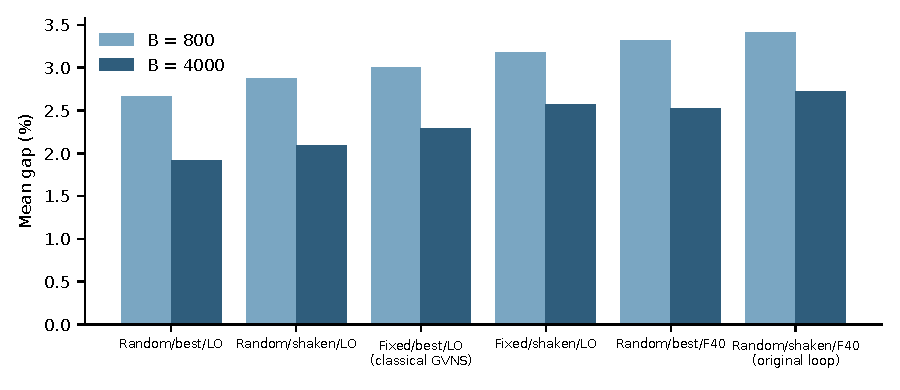
\includegraphics[width=0.8\linewidth]{fig_estrutura.pdf}
\caption{Study 2A: mean gap by search structure (five operators; bars for $B=800$ and $B=4000$).}\label{fig:estrutura}
\end{figure}
\begin{figure}[h]
\centering
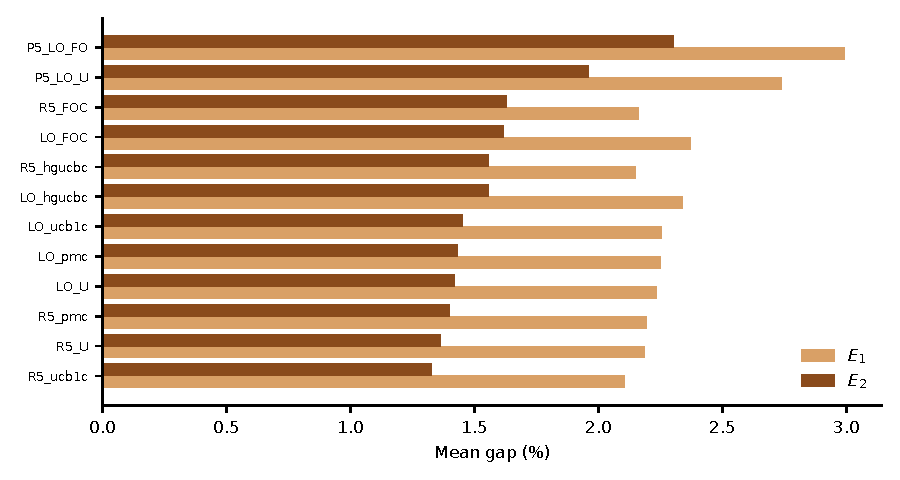
\includegraphics[width=0.8\linewidth]{fig_pool.pdf}
\caption{Study 3: mean gap of every arm at the two budgets (suffix c: cost-aware reward; FOC: fixed order by cost).}\label{fig:pool}
\end{figure}
\begin{figure}[h]
\centering
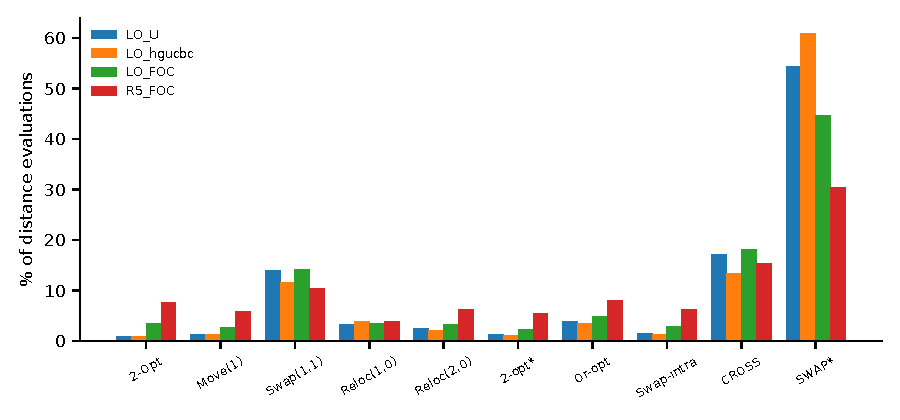
\includegraphics[width=0.8\linewidth]{fig_operadores.pdf}
\caption{Share of distance evaluations spent in each operator at $E_2$ under LO termination (uniform, HG-UCB, fixed order by cost) and under R5 (fixed order by cost).}\label{fig:operadores}
\end{figure}

\section{Operators}\label{app:operators}
Let a solution be a set of routes; $d(\cdot,\cdot)$ is the (symmetric) distance, $0$ the depot, $q$ the demand and $Q$ the capacity. Every operator evaluates its whole neighborhood and applies the move with the most negative cost change $\Delta$ if $\Delta<0$; moves that violate capacity, or that would empty a route when this would violate the route-count constraint, are excluded. Costs change only through the edges listed.
\begin{description}
\item[2-Opt] In a route $(\dots,a,b,\dots,c,d,\dots)$ reverse the segment from $b$ to $c$: $\Delta=d(a,c)+d(b,d)-d(a,b)-d(c,d)$.
\item[Move(1)] Move one customer $u$ with neighbors $p,s$ to another position between $x,y$ of the same route: $\Delta=d(x,u)+d(u,y)-d(x,y)-d(p,u)-d(u,s)+d(p,s)$.
\item[Swap(1,1)] Exchange customers $u\in R_1$ and $v\in R_2$ between routes (each takes the other's place).
\item[Relocate(1,0)] Move one customer from route $R_1$ to any position of route $R_2$.
\item[Relocate(2,0)] Move two consecutive customers, in either orientation, from $R_1$ to any position of $R_2$.
\item[2-opt*] For routes $A$, $B$ and cut points $i,j$, exchange tails: $A'=A_{<i}\,B_{\ge j}$, $B'=B_{<j}\,A_{\ge i}$.
\item[Or-opt(2--3)] Move a segment of two or three consecutive customers, with or without inversion, to another position of the same route.
\item[Swap-intra] Exchange two customers of the same route.
\item[CROSS($\le3$)] Exchange a segment of $l_A$ customers of $A$ with one of $l_B$ customers of $B$, $l_A,l_B\in\{1,2,3\}$, $\max(l_A,l_B)\ge2$, preserving segment orientation.
\item[SWAP*] \citep{vidal2022} Exchange $u\in A$ and $v\in B$, reinserting $u$ at the best position of $B\setminus\{v\}$ and $v$ at the best position of $A\setminus\{u\}$ (not necessarily each other's place). Our version evaluates all pairs without the polar-sector restriction or top-three insertion lists of the original, so it is slower; Study~11 uses a variant with the top-three insertion lists (same best move, \num{s11_cost_ratio} times fewer distance evaluations per application inside the search).
\end{description}
All ten operators were validated against an independent enumeration of their neighborhoods (subsection ``Verification and use of AI tools'' of the manuscript). The shake applies one random move from a randomly chosen original neighborhood, accepted even if it worsens the solution.

\paragraph{TSP neighborhoods (Study 13).} Let a tour be the sequence of the $N-1$ nodes other than node 0, visited between a start and a return to node 0, and $d(\cdot,\cdot)$ the rounded Euclidean distance (EUC\_2D). All nine neighborhoods apply the best improving move. \textbf{2-opt:} reverse a segment, $O(N^2)$ moves. \textbf{Or-opt($k$)}, $k\in\{1,2,3\}$ and $4$--$10$: move a segment of $k$ consecutive nodes, in either orientation, to another position. \textbf{Swap(1,1):} exchange two nodes. \textbf{CROSS($\le3$):} exchange two non-overlapping segments of up to three nodes each. \textbf{3-opt A:} exchange two adjacent segments (a segment insertion of unbounded length), $3\binom{N}{3}$ moves. \textbf{3-opt B:} reverse both of two adjacent segments, $3\binom{N-2}{3}$ moves. The five operators of P5 are 2-opt, Or-opt(1), Swap(1,1), Or-opt(2) and Or-opt(3). The operators are vectorized and each reports the number of distance evaluations that a loop implementation would make (one per new arc; arcs already in the tour are read without counting); both the best move (with the first-in-scan-order tie-break) and the counts match an independent enumeration that builds every neighbor explicitly and recomputes its cost from scratch, in 11\,792 checks over instances of 6 to 31 nodes, and four injected faults (a wrong arc in 3-opt B, a wrong count in CROSS, a wrong mask in Or-opt, a wrong count in 2-opt) are detected. The ALNS destroy operators are the random, worst ($p=3$) and related ($p=6$, by distance only) removals of Study~9 and the segment removal; the repair operators are the greedy, regret-2 and cheapest-insertion (random order) insertions of Study~9.

\section{Hyperparameters}\label{app:hyper}
\begin{table}[h]
\caption{Policy hyperparameters. Defaults are used in Studies 1--3, 6--8, 10 and 11; Study~4 tunes the first four families (default in bold in the grids), and Study~9 tunes UCB1, probability matching, HG-UCB and the adaptive weights of the ALNS on the same grids (selected values in the last rows).}\label{tab:hyper}
\centering\small
\begin{adjustbox}{max width=\linewidth}
\begin{tabular}{lll}
\toprule
Policy & Default & Study 4 grid \\
\midrule
UCB1 & $C=2$ & $C\in\{0.1,0.3,1,\mathbf{2},4\}$ \\
Probability matching & $\gamma=0.1$, $p_{\min}=0.05$ & $\gamma\in\{0.05,\mathbf{0.1},0.3\}\times p_{\min}\in\{0.02,\mathbf{0.05},0.1\}$ \\
HG-UCB & $\alpha=0.5$, $C=2$, $\varepsilon=0.1$, $b_t=0.2$, ADWIN $\delta=0.02$ & $\alpha\in\{0.1,\mathbf{0.5},2\}\times C\in\{1,\mathbf{2},4\}$ \\
Static mixture & uniform & $\theta\in\mathbb{R}^{10}$, $(1{+}4)$ evolution strategy, 15 generations (Studies 4, 10 and 11); $\theta\in\mathbb{R}^{7}$, 8 generations (ALNS, Study 12) \\
Adaptive weights (ALNS, Studies 9 and 12) & $\rho=0.1$, segment 100 & $\rho\in\{0.05,\mathbf{0.1},0.3\}\times$ segment $\in\{50,\mathbf{100},200\}$ \\
$\varepsilon$-greedy & $\varepsilon=0.1$ & not tuned \\
EXP3 & $\gamma=0.1$ & not tuned (Study 6) \\
Thompson sampling & Beta(1,1) prior & not tuned (Study 6) \\
Sliding-window UCB & window 200, $\xi=0.6$ & not tuned (Study 6) \\
Adaptive pursuit & $\alpha=\beta=0.1$, $p_{\min}=0.05$ & not tuned (Study 6) \\
Efficiency UCB & $C=1$ and $C=2$ & not tuned (Study 6) \\
Contextual Thompson sampling & prior strength $k_0=5$, 21 contexts & not tuned (Study 6) \\
HGS-CVRP move order (Study 7) & UCB1 $C=1$; PM $\gamma=0.1$, $p_{\min}=0.05$; HG-UCB-lite $\alpha=0.5$, $C=2$, $\varepsilon=0.1$, $b_t=0.2$ & not tuned \\
Patience (R5) & $r=5$ & not tuned \\
Inner cap (F40) & 40 & not tuned \\
Cost-aware factor & $\mathrm{clip}(\bar g/g,0.1,10)$ & not tuned \\
Static mixture, TSP (Study 13) & uniform & VND: $\theta\in\mathbb{R}^{9}$, 15 generations, 5 seeds; ALNS: $\theta\in\mathbb{R}^{7}$, 8 generations, 3 seeds \\
Selected for the ALNS, TSP (Study 13) & UCB1 $C=\num{s13a_tune_ucb1_C}$; PM $\gamma=\num{s13a_tune_pm_g}$, $p_{\min}=\num{s13a_tune_pm_p}$; HG-UCB $\alpha=\num{s13a_tune_hg_a}$, $C=\num{s13a_tune_hg_C}$; adaptive weights $\rho=\num{s13a_tune_rp_r}$, segment \num{s13a_tune_rp_s}; fixed repair: cheapest insertion in random order & 24 tuning instances \\
Selected for the ALNS (Study 9) & UCB1 $C=2$; PM $\gamma=0.05$, $p_{\min}=0.05$; HG-UCB $\alpha=0.1$, $C=1$; adaptive weights $\rho=0.1$, segment 100 & 24 tuning instances \\
\bottomrule
\end{tabular}
\end{adjustbox}
\end{table}


\section{Detailed design of each study}\label{sup:design}
This section gives the design of each study that the manuscript summarizes: instances, arms, budgets, families of tests and the pre-registration status. Cross-references of the form ``Section~$x$ of the manuscript'' point to the main text.

% DETALHE do desenho por estudo (suplemento, Secao 8). Gerado a partir do desenho original; os rotulos de secao do texto principal viram \mref{...}.
\subsection{Adaptive move selection inside HGS-CVRP (Study 7)}\label{sec:hgsaos}
Study~7 moves the question into a state-of-the-art local search. We use a modified copy of HGS-CVRP \citep{vidal2022} in which, for every pair of nodes, a policy chooses the order in which the applicable route-improvement moves (three relocations, three swaps, 2-opt and two 2-opt* variants) are tried; the first improving move is applied, as in the original, and the policy receives a binary reward (the move improved the solution). SWAP* and the insertion after the depot keep their original order. The arms are the original fixed order, a uniform random order (the non-adaptive control), UCB1, Thompson sampling, probability matching and a lite HG-UCB without the drift detector, with hyperparameters fixed in advance and not tuned (Section~7 of the online supplement). For speed, policy statistics are updated after every attempt but the indices are recomputed in batches of 16 to 256 attempts, an approximation we declare. With the original order the modified code reproduces the solutions of the original program exactly (51 of 51 runs). The budget is a number of generations (offspring), with 250 and 1000 as the primary checkpoints, read from a single run of 4000 generations because the search is deterministic given the seed. Instances are the 25 of sets X and CMT (population P1) and the 30 synthetic validation instances (P2), with ten seeds; sets A and B are excluded because HGS-CVRP converges there within a few hundred generations.

\subsection{A positive control: planted useless operators (Study 8)}\label{sec:s8design}
Null results are only informative if the protocol could have detected an effect. Study~8 therefore plants a heterogeneity of known direction. To the ten operators we add four \emph{useless} operators, each of which, when applied, consumes $X n^2$ distance evaluations and returns ``no improvement'' (it counts as a failure for the patience rule), with $X=4$ or $X=8$; for $n=100$ one application costs 40\,000 or 80\,000 evaluations, against about 13\,000 on average for a real operator (Table~\ref{tab:eff}). The levels were chosen in a pilot on the tuning instances so that uniform selection loses a measurable amount. Uniform selection and the six adaptive policies of the earlier studies run with their default hyperparameters (UCB1, probability matching and HG-UCB with the cost-aware reward, Thompson sampling, EXP3 and the efficiency UCB), on the 74 CVRPLIB instances with ten seeds at $E_1$, in the clean pool and in the two inflated pools (15\,540 runs). The confirmatory family has 12 tests (six adaptive policies $\times$ two inflated pools against uniform selection in the same pool); the share of the planted loss that a policy recovers is exploratory.

\subsection{Adaptive selection in a stochastic large-neighborhood search (Study 9)}\label{sec:s9design}
The studies above use deterministic best-improvement operators, which may be the least favorable setting for adaptation. Study~9 moves to the canonical use of adaptive selection in routing, an adaptive large neighborhood search (ALNS; \citealp{ropke2006}) whose operators are stochastic. Each iteration removes $q\sim U\{\max(5,\lceil0.1n\rceil),\min(\lceil0.3n\rceil,60)\}$ customers with one of four destroy operators (random; worst, with removal-gain rank randomization $p=3$; related, by distance and demand as in \citealp{ropke2006}, $p=6$; whole route) and reinserts them with one of three repair operators (greedy; regret-2; a cheap one that inserts customers in random order at their best position), the two choices being made by two independent instances of the same policy, as in the original method. The result is accepted by simulated annealing with initial temperature $0.02\,c_0/\ln2$ and exponential cooling driven by the fraction of the budget spent (the same for every arm), the budget being $1500\,n^2$ distance evaluations (insertion and relatedness evaluations count; the lengths of existing edges are read without counting). The configuration was fixed on the tuning instances. We use the instances with the ``at least $K$ routes'' convention, the 21 of set X and the 30 synthetic validation instances (ten and five seeds). The arms are uniform selection, the adaptive weights of \citet{ropke2006} (RP; segments of 100 iterations, scores 33, 9 and 13 for a new best, an improvement and an accepted worse solution), UCB1, probability matching, HG-UCB, Thompson sampling, EXP3 and the efficiency UCB; the hyperparameters of RP, UCB1, probability matching and HG-UCB are tuned on the 24 tuning instances by the grid protocol of Study~4 and the others keep their defaults. Two VNS arms at the same budget (uniform selection, and the static mixture of Study~4) serve as a reference for the choice of search structure. The primary test is RP against uniform selection on the 51 instances (one test); the secondary family has 12 tests (six policies, two instance sets) and the tertiary family four (ALNS with uniform selection against the two VNS arms, two sets).

\subsection{Is the gain adaptation? A static control for the ALNS (Study 12)}\label{sec:s12}
The gains of Study~9 could come from learning during the run or merely from weighting the operators better, which a fixed probability vector tuned offline also achieves. Study~12 adds two non-adaptive arms to the ALNS of Study~9: a \emph{static mixture}, with destroy probabilities $\mathrm{softmax}(\theta_{1:4})$ and repair probabilities $\mathrm{softmax}(\theta_{5:7})$ tuned on the 24 tuning instances by the $(1{+}4)$ evolution strategy of Section~\mref{sec:tuning} (eight generations, 33 evaluations of 72 runs each), and a fixed repair (always regret-2, uniform destroy). The new arms run on the same 51 instances, seeds and budget as Study~9 and are compared with the results of that study (same code). The confirmatory family has five tests (static mixture and fixed repair against uniform selection; adaptive weights against each; probability matching against the static mixture), and the central one is adaptive weights against the static mixture.

\subsection{Does the value of selection grow with instance size? (Study 10)}\label{sec:s10design}
A post hoc analysis of the data of Studies 3 and 4 suggested that the static mixture tuned on instances of up to 150 customers beats uniform selection on the larger instances (CVRPLIB instances with more than 120 customers: \num{s10ph_d_1}~pp at $E_1$, \num{s10ph_w_1} wins of \num{s10ph_n_1}, unadjusted $p=\num{s10ph_p_1}$; \num{s10ph_d_5}~pp at $E_2$, $p=\num{s10ph_p_5}$), a pattern that the growing cost of the naive SWAP* neighborhood (Table~\ref{tab:eff}) could explain. Because the subgroup was chosen after the fact, Study~10 tests it on new, larger instances. We generate two further synthetic sets with the same validated generator (and the same reference procedure): a tuning set of 12 instances (200, 300 and 400 customers, four each) and a validation set of 20 instances (200, 300, 400 and 500 customers, five each), disjoint from all other sets. A static mixture is tuned on the tuning set by the $(1{+}4)$ evolution strategy of Section~\mref{sec:tuning} (three seeds); the evaluation compares uniform selection, the mixture of Study~4 (tuned at $n\le150$), the new mixture, and the five online policies (default hyperparameters) on the validation set at $E_1$ with five seeds (800 runs). The confirmatory family has seven tests (each arm against uniform selection).

\subsection{Do the conclusions survive an efficient SWAP*? (Study 11)}\label{sec:s11design}
The SWAP* neighborhood of Studies 3--10 is evaluated naively (all pairs of customers of two routes, all insertion positions); it is much costlier in distance evaluations than the version of HGS-CVRP \citep{vidal2022} (\num{eff_cost_9}~thousand evaluations per application under uniform selection, Table~\ref{tab:eff}) and absorbs \num{s10_swap_n200}--\num{s10_swap_n500}\% of the evaluations on instances of 200 to 500 customers (Study~10). The pool effect (Study~3), the poor showing of cost-aware policies and the absence of gains from selection could therefore be artifacts of that cost. Study~11 replaces the naive SWAP* by an implementation that precomputes, for each customer and route, the three best insertion positions \citep{vidal2022}, without the polar-sector restriction: it returns the same best move as the naive version on all 36 test solutions of six instances, with 4 to 34 times (18 on average) fewer distance evaluations (unit test in the repository). Inside the search, where most applications find no improving move, the mean cost per application falls by a factor of \num{s11_cost_ratio} (Section~\ref{sec:s11}). The pool P10F is the ten-operator pool with this operator; the structure (R5 termination, best acceptance), the budgets $E_1$ and $E_2$, and the instances and seeds are those of Studies 3--6. A static mixture is tuned afresh for P10F on the 24 tuning instances by the evolution strategy of Section~\mref{sec:tuning} (\num{s11_tune_runs} runs). The evaluation compares uniform selection, six online policies (UCB1, probability matching and HG-UCB with the cost-aware reward, Thompson sampling, EXP3 and the efficiency UCB, all with default hyperparameters), the tuned mixture and, for the effect of the pool, uniform selection over the five original operators (P5), on the 74 CVRPLIB instances (ten seeds, $E_1$ and $E_2$) and, without P5, on the 20 large synthetic instances of Study~10 (five seeds, $E_1$): \num{s11_nruns} runs. The confirmatory families have 21 tests (each of the seven non-uniform arms against uniform selection in the three scenarios) and 2 tests (the pool effect at $E_1$ and $E_2$); the comparison with the naive SWAP* of Studies 3 and 6 is descriptive.

\subsection{Does it generalize beyond the CVRP? The traveling salesman problem (Study 13)}\label{sec:s13design}
Studies 1--12 use the CVRP. Study~13 repeats the apparatus on the symmetric Euclidean traveling salesman problem (TSP), which is the CVRP with one vehicle and no capacity limit. It is a modest test of generality by design: the neighborhoods are different operators written anew, but the ALNS reuses the removal and insertion machinery of Study~9. In exchange it offers an independent instance class, a near-optimal reference at low cost and none of the feasibility questions of the CVRP.

\emph{Instances and references.} Evaluation uses \num{s13_nT} EUC\_2D instances of TSPLIB \citep{reinelt1991} with \num{s13_Tmin} to \num{s13_Tmax} nodes (ten seeds; the published optimum is the reference) and \num{s13_nS} synthetic instances with \num{s13_Smin} to \num{s13_Smax} nodes, half uniform and half clustered (five seeds). A disjoint tuning set of 24 synthetic instances (50, 100 and 150 nodes) serves for tuning and calibration. The reference of a synthetic instance is the best of two independent runs of LKH-3 \citep{helsgaun2000}; the two runs agreed on 52 of 54 instances and three further runs confirmed the minimum on the other two. LKH-3 reproduces the published optimum of \num{s13_lkh_ok} of \num{s13_lkh_tot} TSPLIB instances with our cost function, which checks the reader and the rounding convention. The initial solution is the nearest-neighbor tour from node 0, the same for every arm.

\emph{Deterministic regime (VND).} The pool P9 has nine best-improvement neighborhoods: 2-opt, Or-opt(1), Swap(1,1), Or-opt(2), Or-opt(3) (these five, P5, are the analogue of the original five operators), CROSS($\le3$), Or-opt(4--10) and two 3-opt reconnections (exchange of adjacent segments, and reversal of both). A pass costs from about $N^2$ to $N^3/2$ distance evaluations, a ratio of about 60 between the cheapest and the costliest operator in the calibration. The operators are vectorized and the number of evaluations is counted analytically, as a loop implementation would count it; both were validated against an independent brute-force enumeration (11\,792 checks, and four injected faults were detected). The structure and budgets are those of Studies 4--11 (R5 termination, best acceptance, shake with the five operators of P5, $E_1=600\,n^2$ and $E_2=5E_1$ distance evaluations; an exploratory $E_3=25E_1$). At $E_1$ a run applies only about \num{s13_apps_U} operators, so the policies have little time to learn, which $E_2$ and $E_3$ mitigate. The arms are uniform selection, the six online policies of Study~11, a static mixture ($\theta\in\mathbb{R}^9$, tuned by the evolution strategy of Section~\mref{sec:tuning} on the 24 tuning instances at $E_1$: \num{s13_tune_cfg} configurations, 5 seeds) and uniform selection over P5 (the pool effect); the evaluation runs on TSPLIB at $E_1$, $E_2$ and $E_3$ and on the synthetic instances at $E_1$ (\num{s13_nruns_ev} runs). Positive control, as in Study~8: four useless operators of cost $8n^2$ (pool D8) or $16n^2$ (D16) are planted in P9 and the seven arms without the static mixture run on TSPLIB at $E_1$ (\num{s13_nruns_pc} runs).

\emph{Stochastic regime (ALNS).} Four destroy operators (random, worst, related by distance, and \emph{segment}, which removes $q$ consecutive nodes of the tour, replacing the route removal of the CVRP) and three repair operators (greedy insertion, regret-2 and cheapest insertion in random order) with the simulated-annealing acceptance and the budget of Study~9 ($1500\,n^2$ evaluations, each iteration charged $n+1$ for the evaluation of the candidate). Ten arms: uniform selection, the adaptive weights of Ropke and Pisinger, UCB1, probability matching and HG-UCB (tuned on the grids of Study~9 on the tuning instances), Thompson sampling, EXP3 and the efficiency UCB (defaults), a static mixture ($\theta\in\mathbb{R}^7$, eight generations) and a fixed repair (the best single repair operator on the tuning instances, uniform destroy), on the \num{s13a_n} evaluation instances (\num{s13_nruns_a} runs); the deterministic VND at the same budget (uniform over P9, uniform over P5 and the static mixture; \num{s13_nruns_ref} runs) is the reference for comparing the two regimes. One fact about this design was found only in the tuning runs, after the pre-registration: with a single route the regret of the second-best route is undefined, and regret-2 insertion makes the same choices as greedy insertion (the same tours in \num{s13_req_n} of \num{s13_req_tot} random partial solutions, whereas with three routes they differ in \num{s13_req3_n} of \num{s13_req3_tot}; unit test in the repository). The repair set therefore contains two distinct operators and uniform selection gives two thirds of the repairs to one of them. We kept the design, since it was pre-registered, and report the consequence in Section~\ref{sec:s13}.

\emph{Tests.} Pre-registered, with Holm correction by family: VND, 21 tests (each of the seven non-uniform arms against uniform selection in TSPLIB $E_1$, TSPLIB $E_2$ and the synthetic set) and 3 tests of the pool effect; positive control, 12 tests (six policies against uniform selection in each of the two pools); ALNS, one primary test (adaptive weights against uniform selection on the \num{s13a_n} instances), 12 secondary tests (six policies against uniform selection in each set), 4 tertiary tests (static mixture and fixed repair against uniform selection, and adaptive weights against each of them) and 6 structure tests (ALNS with uniform selection against each of the three VND references, by set). Exploratory, labeled as such: $E_3$, the contrasts of the efficiency UCB and Thompson sampling against the static mixture, and the fraction of the planted loss that each policy recovers. After seeing the primary results we added, as \emph{post hoc} analyses not in the pre-registration, a run of the classical VND with a fixed order (the order of the list above, which is that of increasing nominal cost, and its reverse; \num{s13_nruns_x} runs) and the contrasts of the best policies against it, the same three policies with the list of operators shuffled in every run (\num{s13_nruns_q} runs; a test of whether their gain depends on the initialization order), the contrasts against uniform selection over P5 and, in the ALNS, against the static mixture and the fixed repair; they are labeled post hoc wherever they appear.

\subsection{A problem with new constraints: the CVRP with time windows (Study 14)}\label{sec:s14design}
The TSP of Study~13 has neither capacity nor time constraints. Study~14 repeats the deterministic regime on the CVRP with time windows (CVRPTW), where a move that improves the cost may be infeasible in time, so that the neighborhoods must reason about arrival times, and where best-known solutions are published. It covers the descent regime only; the stochastic regime with time windows is Study~16 (Section~\ref{sec:s16design}).

\emph{Instances and cost.} Evaluation uses the \num{s14_nS} instances of \citet{solomon1987} (100 customers; families C1, C2, R1, R2, RC1 and RC2), downloaded from CVRPLIB \citep{cvrplib}, whose reference is the best known solution (proven optimal for all of them). The cost is the total distance with unlimited fleet (at most 25 vehicles), with the CVRPLIB convention that distances and travel times are truncated to one decimal, stored in tenths as integers so that cost and feasibility are exact. Our reader and feasibility simulation reproduce the published cost of the best known solution, and its feasibility, on \num{s14_bks_ok} of \num{s14_bks_tot} instances. A disjoint tuning set of 24 synthetic instances of 100 customers in the style of Solomon (four per family; windows anchored on a feasible sweep route, narrow for the type~1 families and wide for the type~2 families) serves for tuning and calibration; their reference is the best of two runs of PyVRP \citep{wouda2024} of 20~s, which agreed on 21 of 24. The initial solution is a deterministic sequential insertion by increasing due date, the same for every arm.

\emph{Operators.} The pool P9 has nine best-improvement neighborhoods: Move(1) and Swap-intra and Or-opt(2--3) within a route; Swap(1,1), Relocate(1,0), Relocate(2,0) (both orientations), 2-opt* (exchange of route tails), CROSS($\le3$) and CROSS(4--5) between routes. The first five (P5) are the analogue of the original operators. Feasibility in time is checked in constant time per candidate by concatenating precomputed segments \citep{vidal2013}. The operators are implemented in compiled code, and the number of distance evaluations is counted analytically: a candidate that passes the capacity test costs the number of new arcs of the move. Both were validated against an independent brute-force enumeration that builds every neighbor, simulates its feasibility and recomputes its cost from scratch (2\,880 checks with no failure; five injected faults were detected). Under uniform selection at $E_1$ the cost per application ranges from 2\,500 evaluations (Swap-intra) to 103\,000 (CROSS(4--5)), a factor of 42, and the two CROSS neighborhoods absorb \num{s14_cross_U}\% of the evaluations. The structure and budgets are those of Studies 4--13 ($E_1=600\,n^2$, $E_2=5E_1$, exploratory $E_3=25E_1$ distance evaluations, R5 termination, best acceptance, shake with a random feasible move of P5). At $E_1$ a run applies about \num{s14_apps_U} operators.

\emph{Arms.} Uniform selection; the six online policies and the static mixture of Study~13 (the mixture tuned by the evolution strategy of Section~\mref{sec:tuning} on the 24 tuning instances at $E_1$: \num{s14_tune_cfg} configurations, 5 seeds); uniform selection over P5; and three classical fixed-order descents without learning, pre-registered because of Study~13: the order of the list, the order of increasing cost per application measured in the calibration (Swap-intra, Move(1), 2-opt*, Or-opt(2--3), Swap(1,1), Relocate(1,0), Relocate(2,0), CROSS($\le3$), CROSS(4--5)) and its reverse. The evaluation runs on the Solomon instances at $E_1$, $E_2$ and $E_3$ with ten seeds (\num{s14_nruns_ev} runs). Positive control: four useless operators of cost $2n^2$ (pool D2) or $4n^2$ (D4), which raise the gap of uniform selection at $E_1$ in the calibration by 0.69 and 1.44~pp, are planted in P9 and the seven arms without the mixture, P5 and the orders run at $E_1$ (\num{s14_nruns_pc} runs).

\emph{Tests.} Pre-registered, with Holm correction by family: each of the seven non-uniform arms against uniform selection at $E_1$ and $E_2$ (14 tests); the pool effect (2); the three fixed orders against uniform selection at $E_1$ and $E_2$ (6); and, for the positive control, six policies against uniform selection in each pool (12). Exploratory, labeled as such: $E_3$ (11 tests), the efficiency UCB and cost-aware UCB1 and HG-UCB against the cost-ordered descent, the smaller pool and the static mixture (18 tests), and the fraction of the planted loss recovered. Any analysis not in the pre-registration is labeled post hoc where it appears.


\subsection{Is the dead weight of a pool predictive? A prospective test (Study 15)}\label{sec:s15design}
The regularity that policies gain where the pool contains operators that are not worth their cost was formulated after the data of five settings (Section~\mref{sec:r7}). Study~15 turns it into a prediction. In the TSP and in the CVRPTW the nested pools P5 $\subset$ P6 $\subset$ P7 $\subset$ P8 are prefixes of the operator list of Studies 13 and 14. The dead weight $D_k$ of the pool P$k$ is the mean gap of uniform selection over P$k$ minus that over P5, measured at $E_1$ on the 24 synthetic tuning instances of each problem (five seeds). The rule fixed before the evaluation: if $D_k\ge\num{s15_lim}$~pp at least one of the six policies (cost-aware UCB1, probability matching and HG-UCB, Thompson sampling, EXP3, the efficiency UCB, with the defaults of Studies 13 and 14) is significantly better than uniform selection (two-sided Wilcoxon on instance means, Holm over the six within the pool) on the primary set at $E_1$ (TSPLIB; Solomon); otherwise none is. The evaluation adds the fixed-order descent of each pool (list order in the TSP, order of increasing cost restricted to the pool with time windows) and, in the TSP, the 30 synthetic validation instances as an exploratory replication: \num{s15_nruns} runs. The pre-registration is log entry 118 (commit \texttt{bab11eb}).

\subsection{The stochastic regime with time windows: an ALNS for the CVRPTW (Study 16)}\label{sec:s16design}
Study~14 covers the descent regime only, which left open whether the pattern of the ALNS of Studies 9, 12 and 13 (adaptive weights beat uniform selection, but a tuned fixed design does as well) holds when insertions must respect time windows. Study~16 repeats that regime on the Solomon instances of Study~14, with the same arms, tuning protocol and budget as Study~13.

\emph{Operators.} Four destroy operators (random, worst, related and route removal) and three repair operators (greedy insertion, regret-2 and cheapest insertion in random order), chosen by two independent instances of the same policy, as in Study~9. Related removal adds a time term to the distance and demand terms of Shaw (weights 9, 3 and 2 as in \citet{ropke2006} for the VRP with time windows; the time term is the difference of the window starts). Each route stores the start of service of every node and the latest start of service that keeps the rest of the route feasible, so that the feasibility of every insertion position is decided in constant time; costs and times are integers (tenths), hence exact. The complete solution is checked again by simulation in every iteration. Because the distances are truncated to one decimal, the triangle inequality can fail by 0.1 and the removal of a customer can make a tight route infeasible; such candidates are rejected and counted (\num{s16a_inv_U} per run under uniform selection). The operators were validated against independent brute-force implementations that use only the exact simulation of a route: best insertion position and its evaluation count, the exact outcome of the three repairs, the cost bookkeeping and the feasibility of the repaired solution (9\,818 checks, no failure; nine injected faults, among them a missing latest-start test, a strict inequality, ignoring waiting and a sign error in the regret, were all detected), and the complete ALNS returned feasible solutions never below the proven optimum on five Solomon instances (unit test in the repository).

\emph{Budget and temperature.} The budget is $1500\,n^2$ distance evaluations, about 4\,100 iterations per run, each iteration charged $n+R$ evaluations for the candidate, as in Studies 9 and 13. The initial temperature $w_0$ ($T_0=w_0\,c_0/\ln 2$) mattered far more than in the TSP: in the calibration on the tuning instances (three pilots of \num{s16_pilot_runs} runs, the tuning set only) the gap of uniform selection fell from \num{s16p_U_w002}\% at $w_0=0.02$ to \num{s16p_U_w02}\% at $w_0=0.2$. The rule fixed before any data of the study, the same for every arm, was the value of the grid $\{0.02, 0.05, 0.1, 0.2, 0.3, 0.5, 1\}$ that minimizes the mean gap of uniform selection on the tuning instances, so as not to handicap the baseline with a poor temperature: $w_0=0.2$. With it, the fixed regret-2 repair was worse than uniform selection in the calibration (\num{s16p_reg2_w02}\% against \num{s16p_U_w02}\%) and the adaptive weights were slightly better (\num{s16p_RP_w02}\%), unlike in the CVRP, where regret-2 dominated the other repairs.

\emph{Arms and tuning.} Ten arms as in Study~13: uniform selection; the adaptive weights of Ropke and Pisinger, UCB1, probability matching and HG-UCB (tuned on the grids of Study~9 on the 24 tuning instances, three seeds); Thompson sampling, EXP3 and the efficiency UCB (defaults); a static mixture ($\theta\in\mathbb{R}^7$, evolution strategy of eight generations, \num{s16_tune_runs} tuning runs in all together with the grids); and a fixed repair (the best single repair on the tuning instances, uniform destroy). Evaluation: the \num{s16_n} Solomon instances with ten seeds (\num{s16_nruns_a} runs; all feasible). The deterministic VND of Study~14 at the same budget (uniform over P9 and over P5, the descent of increasing cost and the static mixture of the VND; \num{s16_nruns_ref} runs) is the reference for the comparison of the two regimes.

\emph{Tests.} Pre-registered (log entry 121, before any tuning or evaluation data of the study), with Holm correction by family: one primary test (adaptive weights against uniform selection, unadjusted); six secondary tests (the other policies against uniform selection); four tertiary tests (static mixture and fixed repair against uniform selection, adaptive weights against each); fourteen tests of each adaptive policy against each non-adaptive design (the operationalization of ``no policy beats the best fixed design''); and four structure tests (ALNS with uniform selection against each VND reference). Exploratory, labeled as such: the six Solomon classes, equivalence, and the fraction of the gain of the adaptive weights captured by the static mixture and the fixed repair.

\subsection{Adaptive selection of the operator set inside a modern solver: the ILS of PyVRP (Study 17)}\label{sec:s17design}
Study~17 answers the most frequent objection to the earlier studies, that the searches are written in Python and reach gaps of 1.3--3.5\%: it repeats the selection question inside PyVRP~0.13 \citep{wouda2024}, whose iterated local search (ILS: perturbation, granular local search and late-acceptance hill-climbing) reaches a mean gap of \num{s17p_P6_c}\% with its default operators on the tuning instances at 0.1~s per customer.

\emph{What is selected.} The local search of PyVRP scans every pair of neighboring nodes and applies all the operators of its set in turn, so there is no ``next neighborhood'' to choose as in a VND; what a policy can choose at each ILS iteration is the operator set, that is, the strength and the cost of the search. The $k=7$ arms are nested sets: P1 is Exchange(1,0), P2 adds Exchange(2,0), P3 Exchange(1,1), P4 Exchange(2,1), P5 Exchange(2,2), P6 SwapTails (this is the default set of PyVRP for the CVRP) and P7 adds the route operator SwapStar to P6. The initial solution and the exhaustive search that follows every new best solution use P6 in the adaptive arms (the arm's own set in the fixed arms). Policies, reward and tuning are those of the ALNS studies, with one decision per iteration: reward 33 for a new best feasible solution, 9 for an improvement of the current one and 0 otherwise (the acceptance rule of the ILS is not visible to the search), and the efficiency policy is charged the wall time of the call. The module is in the repository (\texttt{src/pyvrp\_aos.py}); with a single set and the same seed it reproduces \texttt{pyvrp.solve} in cost and in number of iterations on five instances and two seeds, the distances and the route costs agree with ours on every tested pair and solution, and all returned solutions satisfy our feasibility convention (unit test in the repository).

\emph{Budget.} The budget is wall-clock time, $T=\nu n$ seconds for $n$ customers, with $\nu=\num{s17_nivel_1}$ and $\num{s17_nivel_2}$ chosen, before any tuning or evaluation data, from the convergence curve of the default set on the tuning instances alone (mean gap \num{s17p_P6_a}, \num{s17p_P6_b} and \num{s17p_P6_c}\% at 0.01, 0.03 and 0.1~s per customer; the first level was discarded because a run lasts 0.5 to 1.5~s, dominated by fixed costs). Eleven processes run in parallel on twelve threads with the tasks shuffled, so the results are not reproducible bit for bit; the number of iterations and the time per set are recorded.

\emph{Instances and arms.} The 74 CVRPLIB instances (ten seeds) and the 30 synthetic validation instances (five seeds), 104 in all; the fleet is capped at $K$ for the sets A and B, which require exactly $K$ routes, and free otherwise, and runs that violate the route-count convention are excluded (\num{s17_ninv} of \num{s17_nruns}). Fourteen arms: the fixed sets P3 to P7 (P1 and P2 are almost useless and appear only in the tuning and as options of the policies), uniform selection over the seven sets, the adaptive weights of Ropke and Pisinger, UCB1, probability matching and HG-UCB (tuned on the grids of Study~9 on the 24 tuning instances, three seeds, at the first budget), Thompson sampling, EXP3 and the efficiency UCB (defaults), and a static mixture ($\theta\in\mathbb{R}^7$, evolution strategy of eight generations; \num{s17_tune_runs} tuning runs in all). The tuned parameters are used at both budgets.

\emph{Tests.} Pre-registered (log entry 124, before any tuning or evaluation data), with Holm correction by family: one primary test (adaptive weights against uniform selection at the first budget, unadjusted); fifteen secondary tests (the other policies and the static mixture against uniform selection at both budgets, and the adaptive weights at the second); eight tests of the ladder of sets (P4$-$P3 to P7$-$P6 at both budgets); four tertiary tests (static mixture against P6 and P7); two tests of uniform selection against the default set; and 21 tests per budget of each adaptive policy against P6, P7 and the static mixture (the operationalization of ``no policy beats the best non-adaptive design''). Exploratory, labeled as such: the two instance sets and the four families of CVRPLIB, and the usage of the sets.


\section{Detailed results by study}\label{sup:results}
% DETALHE dos resultados por estudo (suplemento, Secao 9): o texto completo dos 14 estudos antes da condensacao do texto principal.
Differences are mean paired differences in percentage points (pp) of gap to the reference cost; a negative value favors the first-named arm. Brackets give 95\% bootstrap intervals over instances, $p$ values are Holm-adjusted over the family of the study, and ``wins'' and ``losses'' count the instances (74 CVRPLIB, or 30 synthetic; 25 and 30 in Study 7; the sets of Studies 8--14 are given in their sections) on which the first-named arm has the lower and the higher mean gap. Every number, table and figure of this section is generated from the raw per-run files by scripts (Section~\mref{sec:verification}). All runs of Studies 1--6 and 8--14 were feasible; Study~7 has \num{s7_ninv} exclusions (Section~\ref{sec:s7}).

\subsection{Study 1: does the bandit beat chance?}\label{sec:s1}
Study~1 keeps the original loop (40 inner applications per step) and compares HG-UCB with uniform selection, UCB1, $\varepsilon$-greedy, probability matching and the classical GVNS at a matched budget (Table~\ref{tab:s1}; all contrasts in Table~\stab{tab:s1tests}).

\begin{table}[t]
\caption{Study 1: mean gap (\%) over 74 instances, original loop.}\label{tab:s1}
\centering
\small
\begin{adjustbox}{max width=\linewidth}
\begin{tabular}{lcc}
\toprule
Policy & $B=800$ & $B=4000$ \\
\midrule
Classical GVNS (fixed-order VND) & 3.00 & 2.29 \\
Uniform & 3.41 & 2.72 \\
UCB1 & 3.39 & 2.73 \\
Probability matching & 3.47 & 2.80 \\
HG-UCB (normalized) & 3.47 & 2.83 \\
$\varepsilon$-greedy & 3.50 & 2.86 \\
HG-UCB literal & 4.43 & 4.14 \\
\bottomrule
\end{tabular}
\end{adjustbox}
\end{table}


HG-UCB does not beat uniform selection: \num{s1d_hgucb_norm_uniforme_800}~pp \num{s1ci_hgucb_norm_uniforme_800} at $B=800$ (adjusted $p=\num{s1p_hgucb_norm_uniforme_800}$) and \num{s1d_hgucb_norm_uniforme_4000}~pp \num{s1ci_hgucb_norm_uniforme_4000} at $B=4000$ (adjusted $p=\num{s1p_hgucb_norm_uniforme_4000}$); nor does it differ significantly from UCB1, $\varepsilon$-greedy or probability matching (adjusted $p\ge\num{s1_minp_others_4000}$). The literal variant is \num{s1a_hgucb_literal_hgucb_norm_800}~pp \num{s1ci_hgucb_literal_hgucb_norm_800} and \num{s1a_hgucb_literal_hgucb_norm_4000}~pp \num{s1ci_hgucb_literal_hgucb_norm_4000} worse than normalized HG-UCB, losing on \num{s1l_hgucb_literal_hgucb_norm_800} and \num{s1l_hgucb_literal_hgucb_norm_4000} of 74 instances: the reward scale, not the policy, produces a loss larger than any difference among policies. The classical GVNS has the lowest mean gap and is significantly better than HG-UCB (\num{s1a_hgucb_norm_gvns_classico_800}~pp \num{s1ci_hgucb_norm_gvns_classico_800} and \num{s1a_hgucb_norm_gvns_classico_4000}~pp \num{s1ci_hgucb_norm_gvns_classico_4000}; HG-UCB is worse on \num{s1l_hgucb_norm_gvns_classico_800} and \num{s1l_hgucb_norm_gvns_classico_4000} of 74 instances), a difference examined in Study~2. Of the 12 pre-specified tests, \num{s1_nsig} are significant.

An exploratory run at $B=20\,000$ (\num{sub_n} instances, 5 seeds; low power) shows the same pattern (HG-UCB minus uniform \num{sub_d_hu_20000}~pp, interval containing zero).

\subsection{Study 2: where do the differences come from?}\label{sec:s2}
A diagnostic explains why the original loop is inefficient (all 74 instances, 10 seeds, $B=800$; exploratory). On average \num{diag_ultima}\% of its 40 inner applications per step occur after the last improvement of that step, and \num{diag_otimo}\% occur after all five operators have failed on the current solution (by instance, \num{diag_otimo_min}--\num{diag_otimo_max}\%), when, since every neighborhood is deterministic, no further application can change the solution. The original loop performs \num{sh_f40_800} shakes within 800 applications; random order with local-optimum termination performs \num{sh_ubestlo_800} on average. Study~2 decomposes the structure by crossing operator \emph{order} (fixed or uniformly random), \emph{acceptance} (\textit{best} or \textit{shaken}) and inner-loop \emph{termination} (local optimum, LO, or 40 applications, F40) (Table~\ref{tab:s2a}; all contrasts in Table~\stab{tab:s2tests}).

\begin{table}[t]
\caption{Study 2A: mean gap (\%) over 74 instances by search structure (five operators).}\label{tab:s2a}
\centering
\small
\begin{adjustbox}{max width=\linewidth}
\begin{tabular}{lccc}
\toprule
Order / acceptance / termination & $B=800$ & $B=4000$ & Role \\
\midrule
Random / best / LO & 2.66 & 1.92 & best structure \\
Random / shaken / LO & 2.88 & 2.10 &  \\
Fixed / best / LO & 3.00 & 2.29 & classical GVNS \\
Fixed / shaken / LO & 3.18 & 2.58 &  \\
Random / best / F40 & 3.32 & 2.53 &  \\
Random / shaken / F40 & 3.41 & 2.72 & original loop, uniform \\
\bottomrule
\end{tabular}
\end{adjustbox}
\end{table}


\emph{Termination} is the dominant factor. Stopping at a local optimum instead of running 40 applications improves the gap by \num{g_term_abs}~pp across the two acceptance rules and two budgets (better on \num{g_term_w} of 74 instances; adjusted $p<10^{-4}$ in all four contrasts). \emph{Acceptance} contributes \num{g_acc_abs}~pp (all four contrasts significant, the weakest at adjusted $p=\num{s2p_C3_4000}$; descriptively the effect concentrates in set X, Table~\stab{tab:s2set}). Contrary to our pre-specified expectation, \emph{random order beats fixed order} by \num{g_ord_best_abs}~pp under \textit{best} acceptance and \num{g_ord_shaken_abs}~pp under \textit{shaken}, significantly at both budgets: the fixed order always restarts from 2-Opt, which then absorbs \num{s2_2opt_share_fixed_4000}--\num{s2_2opt_share_fixed_800}\% of all applications. Moving from the original loop to random order, \textit{best} acceptance and LO termination reduces the gap from \num{s2a_gap_uniforme_4000}\% to \num{s2a_gap_s2a_U_best_LO_4000}\% at $B=4000$ with no learning at all.

\paragraph{AOS inside the efficient structure}
In the best structure (\textit{best}/LO, selecting among operators not yet failed) we compare four adaptive policies with random order (rows D1--D4 of Table~\stab{tab:s2tests}). Probability matching ties with random order at both budgets, and UCB1 does at $B=800$ (\num{s2d_D1_800}~pp \num{s2ci_D1_800}); at $B=4000$ UCB1 is marginally worse (\num{s2d_D1_4000}~pp \num{s2ci_D1_4000}, adjusted $p=\num{s2p_D1_4000}$), a difference whose two-level interval \num{rb2_E2_4000_s2b_ucb1_s2a_U_best_LO} includes zero. $\varepsilon$-greedy and HG-UCB are significantly \emph{worse} at both budgets, a result that survives the two-level bootstrap (95\% intervals \num{rb2_E2_800_s2b_eps_greedy_s2a_U_best_LO} and \num{rb2_E2_4000_s2b_eps_greedy_s2a_U_best_LO} for $\varepsilon$-greedy; \num{rb2_E2_800_s2b_hgucb_norm_s2a_U_best_LO} and \num{rb2_E2_4000_s2b_hgucb_norm_s2a_U_best_LO} for HG-UCB). Adaptive policies are better than the classical fixed order by \num{g_vsfixed_abs}~pp, but this reflects the order effect above, not adaptation. Of the 28 pre-specified tests, \num{s2_nsig} are significant.

\subsection{Study 3: a larger, heterogeneous operator pool}\label{sec:s3}
With five similar deterministic operators there may be no room for adaptation. We therefore add 2-opt*, Or-opt (segments of 2--3), an intra-route swap, CROSS exchange (segments up to 3) and a naive SWAP* \citep{vidal2022}, for a pool of ten. The cost of an application differs by a factor of \num{eff_cost_ratio} across operators (mean \num{eff_cost_0}k distance evaluations for 2-Opt, \num{eff_cost_9}k for SWAP*; Table~\ref{tab:eff}) and the budget is therefore measured in distance evaluations (Section~\mref{sec:budgets}). We cross two stopping rules---LO, where adaptation can only reorder, and R5 (stop after five consecutive failures, sampling with replacement), where it can avoid costly useless operators---with five policies (Section~\mref{sec:policies}). Of the 34 pre-specified tests, \num{s3_nsig} are significant (\num{s3_nsig_E1} at $E_1$, \num{s3_nsig_E2} at $E_2$; Table~\ref{tab:s3}; all contrasts in Table~\stab{tab:s3tests}).

\begin{table}[t]
\caption{Study 3: mean gap (\%) over 74 instances (budgets $E_1$ and $E_2$); the last two rows use the original five operators with the same budget.}\label{tab:s3}
\centering
\small
\begin{adjustbox}{max width=\linewidth}
\begin{tabular}{lcc}
\toprule
Arm & $E_1$ & $E_2$ \\
\midrule
R5, UCB1 (cost-aware) & 2.10 & 1.33 \\
R5, uniform & 2.19 & 1.36 \\
R5, probability matching (cost-aware) & 2.19 & 1.40 \\
LO, uniform & 2.23 & 1.42 \\
LO, probability matching (cost-aware) & 2.25 & 1.43 \\
LO, UCB1 (cost-aware) & 2.26 & 1.45 \\
LO, HG-UCB (cost-aware) & 2.34 & 1.56 \\
R5, HG-UCB (cost-aware) & 2.15 & 1.56 \\
LO, fixed order by cost & 2.37 & 1.62 \\
\addlinespace
R5, fixed order by cost & 2.16 & 1.63 \\
Five operators, LO, uniform & 2.74 & 1.96 \\
Five operators, LO, fixed order & 2.99 & 2.30 \\
\bottomrule
\end{tabular}
\end{adjustbox}
\end{table}


\emph{The larger pool is the only large effect:} with the same stopping rule and random order, ten operators beat five by \num{s3a_T1_1}~pp \num{s3ci_T1_1} and \num{s3a_T1_5}~pp \num{s3ci_T1_5} at $E_1$ and $E_2$ (better on \num{s3w_T1_1} and \num{s3w_T1_5} of 74 instances; adjusted $p<10^{-4}$), in all four instance sets (Table~\stab{tab:s3set}). Random order again beats the classical fixed order for the original pool (\num{s3a_T3_1} and \num{s3a_T3_5}~pp). A fixed order \emph{by cost} is worse than random order with the large pool (\num{s3d_LO_FOCvsU_1} and \num{s3d_LO_FOCvsU_5}~pp under LO; \num{s3d_R5_FOCvsU_5}~pp under R5 at $E_2$). \emph{No adaptive policy beats uniform selection:} UCB1 and probability matching tie with it under both stopping rules and budgets, and HG-UCB is significantly worse at $E_2$ (\num{s3d_LO_hgucbcvsU_5}~pp \num{s3ci_LO_hgucbcvsU_5} under LO, \num{s3d_R5_hgucbcvsU_5}~pp \num{s3ci_R5_hgucbcvsU_5} under R5). UCB1 and probability matching do beat the fixed order by cost at $E_2$ (by \num{g_s3_vsfoc_abs}~pp), which reflects the weakness of that order. The cost-aware reward made no measurable difference to HG-UCB (\num{rbd_E3_1_s3_R5_hgucbc_s3_R5_hgucb_cego} and \num{rbd_E3_5_s3_R5_hgucbc_s3_R5_hgucb_cego}~pp at $E_1$ and $E_2$, intervals \num{rb1_E3_1_s3_R5_hgucbc_s3_R5_hgucb_cego} and \num{rb1_E3_5_s3_R5_hgucbc_s3_R5_hgucb_cego}). The stopping rule (R5 versus LO) has no detectable effect under random order (\num{s3d_T2_1} and \num{s3d_T2_5}~pp, not significant).

Uniform and adaptive policies spend \num{s3_swap_min}--\num{s3_swap_max}\% of their distance evaluations in SWAP* (the fixed order by cost, \num{s3_swap_foc_min}--\num{s3_swap_foc_max}\%), with HG-UCB concentrating the most (\num{s3_swap_hg_lo}\% under LO; Figure~S3 of the supplement). This concentration is a cost effect, not an efficiency one: SWAP* has the highest success rate per application (\num{eff_suc_9}\%) but the lowest relative gain per thousand distance evaluations, \num{eff_ratio} times below 2-Opt (Table~\ref{tab:eff}). Whether the benefit of the larger pool comes from the cheap or from the expensive additions is tested in Study~5.

\begin{table}[t]
\caption{Efficiency of each operator under uniform selection (R5, ten operators, $E_1$, 74 instances, 10 seeds): success rate per application, mean relative gain per success, mean cost per application (thousand distance evaluations) and relative gain (\%) per thousand distance evaluations, sorted by the last column.}\label{tab:eff}
\centering
\small
\begin{adjustbox}{max width=\linewidth}
\begin{tabular}{lcccc}
\toprule
Operator & Success (\%) & Gain/success (\%) & Cost (k eval.) & Gain per 1k eval. (\%) \\
\midrule
2-Opt & 37.3 & 1.10 & 1.1 & 0.364 \\
Move(1) & 38.7 & 1.06 & 1.9 & 0.219 \\
2-opt* & 24.3 & 1.45 & 1.8 & 0.192 \\
Swap-intra & 30.3 & 1.07 & 2.0 & 0.166 \\
Reloc(1,0) & 33.4 & 1.50 & 4.5 & 0.111 \\
Or-opt(2-3) & 37.2 & 1.23 & 5.2 & 0.088 \\
Reloc(2,0) & 10.6 & 2.34 & 3.8 & 0.065 \\
Swap(1,1) & 24.4 & 1.51 & 18.9 & 0.019 \\
CROSS & 21.5 & 1.48 & 24.7 & 0.013 \\
SWAP* & 40.0 & 1.55 & 70.9 & 0.009 \\
\bottomrule
\end{tabular}
\end{adjustbox}
\end{table}


\subsection{Study 4: tuned policies, a tuned static mixture and independent instances}\label{sec:s4}
Study~4 gives adaptation its best chance and measures the headroom. The hyperparameters of UCB1, probability matching and HG-UCB were tuned with one protocol (24 synthetic tuning instances disjoint from the evaluation instances, R5 structure at $E_1$, five seeds common to all configurations, grids of 5, 9 and 9 points; Section~7 of the online supplement), and a \emph{static mixture}---a fixed probability vector over the ten operators, with no learning---was tuned on the same instances by a $(1{+}4)$ evolution strategy (61 evaluations; weights in Table~\stab{tab:s4pesos}). Table~\stab{tab:s4config} lists the selected values. The gains of tuning on the tuning set are small for the three policies (\num{s4_tune_ucb1_d}\% to \num{s4_tune_ucb1_t}\% for UCB1, \num{s4_tune_pm_d}\% to \num{s4_tune_pm_t}\% for probability matching, \num{s4_tune_hgucb_d}\% to \num{s4_tune_hgucb_t}\% for HG-UCB) and of the order of the tuning noise: uniform selection implemented as an equal-weight static mixture differs from the uniform-selection arm by \num{s4_tune_noise}~pp on the same instances (different consumption of random numbers). The tuned static mixture, by contrast, improves the tuning-set gap from \num{s4_tune_static0}\% (equal weights) to \num{s4_tune_static_best}\%.



On the 74 CVRPLIB instances (Table~\stab{tab:s4tests}), \emph{no tuned policy beats uniform selection}: UCB1 \num{s4d_V1_1} and \num{s4d_V1_5}~pp, probability matching \num{s4d_V2_1} and \num{s4d_V2_5}~pp at $E_1$ and $E_2$ (no test significant), and tuned HG-UCB is significantly worse at $E_2$ (\num{s4d_V3_5}~pp \num{s4ci_V3_5}, adjusted $p=\num{s4p_V3_5}$). The improvement on the tuning set does not transfer: tuned UCB1 is no better than its default on CVRPLIB (\num{s4_gap_ucb1_t_1}\% against \num{s4_gap_ucb1_d_1}\% at $E_1$, \num{s4_gap_ucb1_t_5}\% against \num{s4_gap_ucb1_d_5}\% at $E_2$), as expected when the best of several noisy evaluations is selected. The \emph{static mixture} is at best marginally better than uniform selection: \num{s4d_V4_1}~pp \num{s4ci_V4_1} at $E_1$ (adjusted $p=\num{s4p_V4_1}$) and \num{s4d_V4_5}~pp \num{s4ci_V4_5} at $E_2$. Even with a distribution tuned offline on 24 instances, the gain over uniform selection is \num{s4a_V4_1}~pp at the smaller budget (not significant after correction) and null at the larger one, a benchmark for what a single global operator distribution can add. No tuned policy beats the static mixture (\num{s4d_V5_1}, \num{s4d_V6_1} and \num{s4d_V7_1}~pp at $E_1$ for UCB1, probability matching and HG-UCB; probability matching is significantly worse, adjusted $p=\num{s4p_V6_1}$). Of the 14 tests, \num{s4_nsig74} are significant, and in both the adaptive policy is the worse arm.

The learned mixture concentrates \num{s4_wp_2opt_pair}\% of its probability on 2-Opt and 2-opt*, two of the cheapest and most efficient operators, and only \num{s4_wp_expensive}\% on the three expensive ones, Swap(1,1), CROSS and SWAP* (Table~\stab{tab:s4pesos}), consistent with the per-evaluation efficiencies of Table~\ref{tab:eff}; it gives SWAP* only \num{s4_wp9}\% of its selections (although SWAP* absorbs \num{s4_static_swap_1}\% of its evaluations because of its cost), so the pool benefit does not require frequent use of the most expensive operator.

On the 30 synthetic validation instances (up to 300 customers, 5 seeds, $E_1$; Table~\stab{tab:s4val}) the pool effect replicates (\num{s4d_W1}~pp \num{s4ci_W1}, adjusted $p<10^{-4}$), whereas the effect of the fixed order by cost does not (\num{s4d_W2}~pp, adjusted $p=\num{s4p_W2}$) and no tuned policy differs from uniform selection (UCB1 \num{s4d_W3}, probability matching \num{s4d_W4}, HG-UCB \num{s4d_W5}~pp). The static mixture is \num{s4d_W6}~pp \num{s4ci_W6} from uniform selection (adjusted $p=\num{s4p_W6}$). Of the 6 tests, \num{s4_nsigval} is significant.

\subsection{Study 5: which operators explain the pool effect?}\label{sec:s5}
Table~\ref{tab:eff} suggests that the cheap operators are far more efficient than the expensive ones, so we expected the cheap additions to explain the benefit of the larger pool. Study~5 tests this with uniform selection on subsets of the pool (Table~\stab{tab:s5}): P8c adds 2-opt*, Or-opt and Swap-intra to the original five (P5), P7e adds CROSS and SWAP*, and P7c removes Swap(1,1), CROSS and SWAP* from the ten. \emph{The expectation is refuted:} the expensive pair is at least as valuable as the cheap trio. Adding the three cheap operators improves the gap by \num{g_s5_A1}~pp (range over the two stopping rules and the two budgets), whereas adding only CROSS and SWAP* improves it by \num{g_s5_A2}~pp and recovers \num{s5_rec_P7e_rng}\% of the effect of the full pool, against \num{s5_rec_P8c_rng}\% for the cheap trio (A1 and A2: all eight tests significant; Table~\stab{tab:s5tests}). The expensive operators still add value on top of the cheap ones (A3, \num{g_s5_A3}~pp, significant in \num{s5_A3_nsig} of 4 cases), removing Swap(1,1), CROSS and SWAP* from the ten operators costs \num{g_s5_A4}~pp (A4, significant in \num{s5_A4_nsig} of 4 cases), and even removing only Swap(1,1) from the eight-operator pool costs \num{g_s5_A5}~pp (A5, significant in \num{s5_A5_nsig} of 4 cases). Of the 20 pre-specified tests, \num{s5_nsig} are significant.


The operators that Table~\ref{tab:eff} ranks as least efficient therefore contribute substantially. Under uniform selection SWAP* absorbs \num{s5_p7e_swap_1}\% of the distance evaluations in P7e (CROSS \num{s5_p7e_cross_1}\%), and the tuned static mixture of Study~4 reaches a gap not significantly different from that of uniform selection over the ten operators while spending \num{s4_static_swap_1}\% of its evaluations on SWAP* instead of \num{s3_U_swap_1}\%. The per-evaluation efficiency measured under uniform selection thus understates the value of costly operators. A direct, exploratory diagnostic explains why: at \num{compl_n} local optima of the five original operators (74 instances, 3 seeds, 8 local optima each, reached by a fixed-order descent after a shake), one application of the best-improvement move of SWAP* finds an improvement in \num{compl_swapstar}\% of the cases and CROSS in \num{compl_cross}\%, against \num{compl_2opt}\% for 2-opt*, \num{compl_oropt}\% for Or-opt and \num{compl_swapintra}\% for Swap-intra; in \num{compl_so_caros}\% of the local optima only CROSS or SWAP* find an improvement, and in \num{compl_so_baratos}\% only the cheap added operators do. The expensive operators are complementary to the original ones: they improve solutions on which the cheap neighborhoods have failed.

\subsection{Study 6: further policy families and contextual policies}\label{sec:s6}
Study~6 asks whether the null results are specific to the four policy families examined so far. In the structure of Study~4 (R5, ten operators) and without tuning, we add EXP3, Thompson sampling, sliding-window UCB, adaptive pursuit, an efficiency UCB that charges the cost of every application (two exploration constants) and two contextual Thompson policies (Section~\mref{sec:policies}; Table~\ref{tab:s6}).

\inputopt{tab_s6}

\emph{No policy beats uniform selection:} none of the 16 pre-specified tests shows an improvement, and in \num{s6_nsig} of them the policy is significantly worse (Table~\ref{tab:s6}). EXP3 and sliding-window UCB are indistinguishable from uniform selection at both budgets (EXP3 \num{s6d_W1_1} and \num{s6d_W1_5}~pp, sliding-window UCB \num{s6d_W3_1} and \num{s6d_W3_5}~pp at $E_1$ and $E_2$). Thompson sampling and adaptive pursuit are worse (\num{s6d_W2_1} and \num{s6d_W2_5}~pp; \num{s6d_W4_1} and \num{s6d_W4_5}~pp), and so are the two contextual policies at $E_2$ (\num{s6d_W7_5} and \num{s6d_W8_5}~pp). The policy that charges the cost of every application is the worst of the study: with $C=1$ it is \num{s6d_W5_1} and \num{s6d_W5_5}~pp worse than uniform selection at $E_1$ and $E_2$, and with $C=2$ it is \num{s6d_W6_5}~pp worse at $E_2$. It does what it is designed to do, moving evaluations to cheap operators (at $E_2$, 2-Opt receives \num{s6_eff_2opt_5}\% of its evaluations and SWAP* \num{s6_eff_swap_5}\%, against \num{s3_U_2opt_5}\% and \num{s3_U_swap_5}\% under uniform selection), and, in line with Study~5, it loses because the expensive operators are worth more than their measured efficiency suggests. On the 30 synthetic validation instances (exploratory, $E_1$, no multiplicity correction) \num{s6v_nworse_raw} of the eight arms are nominally worse than uniform selection and one, sliding-window UCB, is nominally better (\num{s6vd_3}~pp \num{s6vci_3}, unadjusted $p=\num{s6vp_3}$); this difference does not survive a Holm correction over the eight comparisons (adjusted $p=\num{s6vph_3}$) and is not seen on CVRPLIB (\num{s6d_W3_1} and \num{s6d_W3_5}~pp).

\subsection{Study 7: adaptive move selection inside HGS-CVRP}\label{sec:s7}
Study~7 asks whether the null results hold inside a state-of-the-art local search (Section~\ref{sec:hgsaos}; Table~\ref{tab:s7}). They do, but the test is weak, because within HGS-CVRP the order in which the moves of a node pair are tried hardly matters. None of the 20 pre-specified tests is significant, the largest difference in absolute value is \num{s7_maxabs}~pp (\num{s7_maxabs_adapt}~pp for adaptive policies), and the original order does not differ significantly from the uniform random order either (on the synthetic instances at 250 generations it is \num{s7a_fixed_P2_250}~pp worse, interval \num{s7ci_fixed_P2_250}, whose lower limit is above zero, but the Wilcoxon test gives raw $p=\num{s7pr_fixed_P2_250}$). The minimum detectable effect at 80\% power is \num{s7_mde_med}~pp (median over the 20 tests). Of the 16 contrasts of adaptive policies at the primary checkpoints, \num{s7_neq} are equivalent to the random order within $\pm0.05$~pp, and so are all \num{s7_late_n} contrasts at 2000 and 4000 generations (exploratory). Including the \num{s7_ninv} runs excluded for violating the route-count bound of our convention (all on one instance, X-n195-k51) changes nothing (\num{s7_sens_nsig} significant tests). There is structure to learn, since the success rate per attempt varies by a factor of \num{s7_succ_ratio} across move types (from \num{s7_succ_2} to \num{s7_succ_4} improving moves per $10^4$ attempts under the random order), but because the first improving move is applied and a pair rarely admits several, ordering has little leverage, as a comment in the HGS-CVRP code notes. Budgets are matched in generations, not in CPU time: a generation takes \num{s7_cpu_fixed}~ms of CPU with the original order, \num{s7_cpu_unif}~ms with the uniform random order and \num{s7_cpu_ts}--\num{s7_cpu_hg}~ms with Thompson sampling to HG-UCB (probability matching, \num{s7_cpu_pm}~ms, suffers from floating-point underflow of its estimates, an implementation artifact). The original order is the fastest, so at equal CPU time it would beat every learned order, whereas the cost differences among the learned and random orders reflect our implementation. Because even randomizing the order changes so little, the study shows that nothing is gained at this decision point of HGS-CVRP; it is not evidence about other decision points of the solver.

\inputopt{tab_s7}

\subsection{Study 8: a positive control with planted useless operators}\label{sec:s8}
The null results above could reflect an insensitive protocol rather than the absence of exploitable structure. Study~8 (Section~\ref{sec:s8design}) adds four useless operators to the pool. Under uniform selection they absorb \num{s8_duds_D4x4_U}\% and \num{s8_duds_D4x8_U}\% of the distance evaluations and raise the gap by \num{s8_loss_D4x4}~pp and \num{s8_loss_D4x8}~pp (Table~\ref{tab:s8}). Of the 12 pre-specified tests, \num{s8_nsig} are significant, all in favor of the adaptive policy, so the protocol is not blind: Thompson sampling is \num{s8a_D4x8_ts}~pp better than uniform selection in the $8n^2$ pool (\num{s8ci_D4x8_ts}, adjusted $p=\num{s8p_D4x8_ts}$), the efficiency UCB \num{s8a_D4x8_eff}~pp (\num{s8ci_D4x8_eff}, $p=\num{s8p_D4x8_eff}$) and the cost-aware HG-UCB \num{s8a_D4x8_hgucbc}~pp ($p=\num{s8p_D4x8_hgucbc}$); in the $4n^2$ pool only UCB1 is significant (\num{s8a_D4x4_ucb1c}~pp, $p=\num{s8p_D4x4_ucb1c}$).

\begin{table}[t]
\caption{Study 8 (positive control): mean gap (\%) over 74 instances at $E_1$ in the clean pool of ten operators and in pools with four planted useless operators (each costing $4n^2$ or $8n^2$ distance evaluations and never improving); in parentheses, the difference from uniform selection \emph{in the same pool} in pp (* marks Holm-significance over the 12 confirmatory tests; clean-pool comparisons are exploratory).}\label{tab:s8}
\centering
\small
\begin{adjustbox}{max width=\linewidth}
\begin{tabular}{lccc}
\toprule
Policy & Clean pool & 4 useless, $4n^2$ & 4 useless, $8n^2$ \\
\midrule
Uniform selection & 2.19 & 2.55 & 2.72 \\
UCB1 (cost-aware) & 2.10 ($-$0.08) & 2.48 ($-$0.07*) & 2.67 ($-$0.05) \\
Probability matching (cost-aware) & 2.19 ($+$0.01) & 2.48 ($-$0.07) & 2.68 ($-$0.05) \\
HG-UCB (cost-aware) & 2.15 ($-$0.04) & 2.54 ($-$0.01) & 2.65 ($-$0.07*) \\
Thompson sampling & 2.32 ($+$0.14) & 2.43 ($-$0.12) & 2.51 ($-$0.22*) \\
EXP3 & 2.19 ($+$0.01) & 2.54 ($-$0.01) & 2.74 ($+$0.01) \\
Efficiency UCB & 2.48 ($+$0.29) & 2.50 ($-$0.05) & 2.56 ($-$0.16*) \\
\bottomrule
\end{tabular}
\end{adjustbox}
\end{table}


The policies differ sharply in how much of the planted loss they recover (exploratory; Table~\stab{tab:s8rec}). The efficiency UCB recovers \num{s8rec_D4x8_eff}\% of it in the $8n^2$ pool (interval \num{s8reci_D4x8_eff}) and Thompson sampling \num{s8rec_D4x8_ts}\% (\num{s8reci_D4x8_ts}), cutting the share of evaluations wasted on useless operators from \num{s8_duds_D4x8_U}\% to \num{s8_duds_D4x8_eff}\% and \num{s8_duds_D4x8_ts}\%; UCB1, probability matching, HG-UCB and EXP3 with default hyperparameters recover at most \num{s8rec_D4x8_pmc}\%, and keep spending \num{s8_duds_D4x8_hgucbc}--\num{s8_duds_D4x8_exp3}\% of the evaluations on the useless operators. For probability matching a structural reason is the exploration floor: with $p_{\min}=0.05$ and $k=10$ or 14 operators, 50\% or 70\% of the probability mass is reserved for uniform selection. Insurance has a premium: in the clean pool Thompson sampling and the efficiency UCB are significantly worse than uniform selection (\num{s8d_P10_ts} and \num{s8d_P10_eff}~pp, exploratory), and even the best policy in an inflated pool stays above uniform selection in the clean pool, so the best defense against a bad pool remains not to build one. The ceiling of what a policy can protect is itself small, because of diminishing returns of the budget: wasting \num{s8_duds_D4x8_U}\% of the evaluations costs only \num{s8_loss_D4x8}~pp.

\subsection{Study 9: adaptive selection in a stochastic large-neighborhood search}\label{sec:s9}
Study~9 (Section~\ref{sec:s9design}) is the first setting in which adaptive selection helps. The adaptive weights of Ropke and Pisinger are \num{s9prim_a}~pp better than uniform selection on the \num{s9_n_inst} instances (\num{s9prim_ci}; \num{s9prim_w} wins and \num{s9prim_l} losses; $p<10^{-4}$ in the single primary test), which lowers the mean gap from \num{s9_gap_U}\% to \num{s9_gap_RP}\% (Table~\ref{tab:s9}). Of the 12 secondary tests, \num{s9_nbetter} favor the adaptive policy after Holm correction: probability matching with the tuned $\gamma=0.05$ (\num{s9d_pm_X}~pp on set X and \num{s9d_pm_V}~pp on the synthetic set), EXP3 (\num{s9d_exp3_X} and \num{s9d_exp3_V}~pp) and HG-UCB on set X (\num{s9d_hgucb_X}~pp). UCB1 does not differ from uniform selection, and Thompson sampling and the efficiency UCB are much worse (\num{s9d_ts_V} and \num{s9d_eff_X}~pp on the sets where they are significant). The usage statistics show the mechanism: RP, UCB1 and probability matching move the repair choice to regret-2 (\num{s9_reg2_RP}\%, \num{s9_reg2_ucb1}\% and \num{s9_reg2_pm}\% of the repair choices, against \num{s9_reg2_U}\% under uniform selection), the operator that dominates the other two here. This heterogeneity of quality, which the best-improvement operators of the VNS do not have, is what the policies exploit, in line with the positive control of Study~8; the same two policies that were best against useless operators (Thompson sampling, the efficiency UCB) concentrate too early on the cheap or random operators and lose, so the choice of policy depends on the kind of heterogeneity.

\begin{table}[t]
\caption{Study 9 (ALNS with stochastic destroy and repair operators, $1500\,n^2$ distance evaluations): mean gap (\%) on the 21 instances of set X (ten seeds) and the 30 synthetic validation instances (five seeds); in parentheses, the difference from uniform selection in pp (* marks Holm-significance over the 12 secondary tests; for the adaptive weights, the primary test on the 51 instances is in the text and the per-set differences are exploratory). The last rows are VNS arms at the same budget.}\label{tab:s9}
\centering
\small
\begin{adjustbox}{max width=\linewidth}
\begin{tabular}{lcc}
\toprule
Policy & Set X & Synthetic validation \\
\midrule
Uniform selection & 1.48 & 1.86 \\
Adaptive weights (Ropke--Pisinger) & 1.24 ($-$0.24) & 1.42 ($-$0.44) \\
UCB1 & 1.74 ($+$0.26) & 2.20 ($+$0.34) \\
Probability matching & 1.15 ($-$0.33*) & 1.40 ($-$0.46*) \\
HG-UCB & 1.31 ($-$0.16*) & 1.60 ($-$0.26) \\
Thompson sampling & 2.63 ($+$1.16) & 3.04 ($+$1.18*) \\
EXP3 & 1.21 ($-$0.27*) & 1.52 ($-$0.34*) \\
Efficiency UCB & 3.45 ($+$1.97*) & 3.81 ($+$1.95*) \\
VNS, uniform selection (same budget) & 3.15 & 2.92 \\
VNS, static mixture (same budget) & 2.72 & 2.58 \\
\bottomrule
\end{tabular}
\end{adjustbox}
\end{table}


The search structure matters more than the selection layer: at the same budget, ALNS with uniform selection is better than VNS with uniform selection by \num{s9ta_vns_U_X} (set X) and \num{s9ta_vns_U_V}~pp (synthetic set), and better than VNS with the tuned static mixture by \num{s9ta_vns_static_X} and \num{s9ta_vns_static_V}~pp (Holm-adjusted $p\le0.002$ in the four tests). Two cautions apply. The gains of the adaptive policies are two to three times the average adaptive layer of the ALNS literature, and a fixed probability vector tuned offline might capture the same gain, since it can also learn that regret-2 is the best repair; this control is the object of Study~12 (Section~\ref{sec:s12}).

\subsection{Study 12: is the gain of the ALNS adaptation?}\label{sec:s12res}
It is not (Section~\ref{sec:s12}; Table~\ref{tab:s12}). A static mixture tuned offline (destroy probabilities \num{s12_wd_0}, \num{s12_wd_1}, \num{s12_wd_2} and \num{s12_wd_3}\% for random, worst, related and route removal; repair probabilities \num{s12_wr_0}, \num{s12_wr_1} and \num{s12_wr_2}\% for greedy, regret-2 and the cheap repair) is \num{s12a_static_U}~pp better than uniform selection (\num{s12ci_static_U}, adjusted $p<10^{-3}$), and the adaptive weights do not differ from it (\num{s12d_RP_static}~pp, \num{s12ci_RP_static}, adjusted $p=\num{s12p_RP_static}$); the static mixture captures \num{s12cap_static}\% of the gain of the adaptive weights over uniform selection (interval \num{s12capci_static}), and probability matching, the best adaptive arm, is \num{s12d_pm_static}~pp from it (adjusted $p=\num{s12p_pm_static}$). The simplest control does best: always using the regret-2 repair, with uniform destroy, is \num{s12a_reg2_U}~pp better than uniform selection and \num{s12a_RP_reg2}~pp \emph{better} than the adaptive weights (\num{s12ci_RP_reg2}; adjusted $p=\num{s12p_RP_reg2}$), the price of having to learn which repair is the best.

\begin{table}[t]
\caption{Study 12 (static control for the ALNS): mean gap (\%) on set X (21 instances), the synthetic validation set (30) and both (51), and the difference from uniform selection over the 51 instances in pp. The static mixture and the fixed repair are new arms; the other rows are the corresponding arms of Study 9 (same code, instances and seeds).}\label{tab:s12}
\centering
\small
\begin{adjustbox}{max width=\linewidth}
\begin{tabular}{lcccc}
\toprule
Policy & Set X & Synthetic & All & Difference \\
\midrule
Uniform selection & 1.48 & 1.86 & 1.70 \\
Static mixture (tuned offline) & 1.16 & 1.45 & 1.33 & $-$0.37 \\
Fixed repair: always regret-2 & 1.16 & 1.29 & 1.23 & $-$0.47 \\
Adaptive weights (Ropke--Pisinger) & 1.24 & 1.42 & 1.34 & $-$0.36 \\
Probability matching (tuned) & 1.15 & 1.40 & 1.30 & $-$0.40 \\
\bottomrule
\end{tabular}
\end{adjustbox}
\end{table}


The gain of Study~9 is therefore a gain from weighting the operators well, not from adapting during the run. What the adaptive policies provide is that discovery without tuning: the adaptive weights reach the level of the tuned mixture with no tuning run, whereas the mixture needed \num{s12_tune_runs} tuning runs (and a tuning gap of \num{s12_tune_gap}\% against \num{s12_tune_eq}\% for equal weights). This is consistent with the tuned static mixture of Study~4 and with Study~10, where no policy ever beat the best fixed configuration, and it sharpens the conclusion of the paper: adaptation recovers a good fixed configuration when none is available, but we found no setting in which it exceeds one.

\subsection{Study 10: larger instances}\label{sec:s10}
The pattern that motivated Study~10 does not replicate (Section~\ref{sec:s10design}; Table~\ref{tab:s10}). On the \num{s10_n_inst} new instances of 200 to 500 customers no mixture or policy is significantly better than uniform selection after correction: the mixture of Study~4 is \num{s10a_static_S}~pp better (\num{s10ci_static_S}; unadjusted $p=\num{s10pr_static_S}$, adjusted $p=\num{s10p_static_S}$) and the mixture tuned at this size \num{s10a_static_L}~pp better (\num{s10ci_static_L}; adjusted $p=\num{s10p_static_L}$), with a minimum detectable effect of \num{s10mde_static_L}--\num{s10mde_static_S}~pp at 80\% power; the three cost-aware online policies are within \num{s10a_ucb1c}~pp of uniform selection, and Thompson sampling and the efficiency UCB are significantly \emph{worse} (\num{s10d_ts} and \num{s10d_eff}~pp). The advantage of the mixtures does not grow with $n$: for the mixture tuned at this size it is \num{s10dn200_static_L}, \num{s10dn300_static_L}, \num{s10dn400_static_L} and \num{s10dn500_static_L}~pp at 200, 300, 400 and 500 customers (Spearman correlation with $n$ \num{s10rho_static_L}, $p=\num{s10rhop_static_L}$, the wrong sign for the hypothesis). The naive SWAP* absorbs \num{s10_swap_n200}--\num{s10_swap_n500}\% of the evaluations under uniform selection, so these instances are a demanding setting for any policy, yet tuning on them (gap \num{s10_tune_gap_eq}\% with equal weights, \num{s10_tune_gap_L}\% after the search) did not transfer. We conclude that the subgroup pattern of the earlier data was a selection effect, and that a mixture learned offline yields at best a few tenths of a point, with large variance.

\begin{table}[t]
\caption{Study 10: instances of 200 to 500 customers (20 synthetic validation instances, five seeds, $E_1$): mean gap (\%), mean paired difference from uniform selection in pp [95\% CI], unadjusted $p$ and Holm-adjusted $p$ over seven tests.}\label{tab:s10}
\centering
\small
\begin{adjustbox}{max width=\linewidth}
\begin{tabular}{lcccc}
\toprule
Policy & Gap & Difference & $p$ & $p$ (Holm) \\
\midrule
Uniform selection & 4.44 & & &  \\
Static mixture tuned at $n\le150$ (Study 4) & 4.04 & $-$0.40 [$-$0.69, $-$0.13] & 0.027 & 0.13 \\
Static mixture tuned at $n=200$--400 & 4.30 & $-$0.14 [$-$0.25, $-$0.04] & 0.030 & 0.13 \\
UCB1 (cost-aware) & 4.35 & $-$0.09 [$-$0.20, 0.02] & 0.143 & 0.43 \\
Probability matching (cost-aware) & 4.38 & $-$0.06 [$-$0.22, 0.11] & 0.498 & 0.52 \\
HG-UCB (cost-aware) & 4.41 & $-$0.03 [$-$0.13, 0.08] & 0.261 & 0.52 \\
Thompson sampling & 4.64 & $+$0.20 [0.10, 0.32] & 0.001 & 0.006 \\
Efficiency UCB & 4.68 & $+$0.24 [0.04, 0.43] & 0.008 & 0.050 \\
\bottomrule
\end{tabular}
\end{adjustbox}
\end{table}


\subsection{Study 11: do the results survive an efficient SWAP*?}\label{sec:s11}
They do (Section~\ref{sec:s11design}; Table~\ref{tab:s11}). Under uniform selection the efficient SWAP* costs \num{s11_cost_fast} thousand distance evaluations per application, against \num{eff_cost_9} for the naive one, and its share of the evaluations falls from \num{s11_swap_naive}\% in Study~3 to \num{s11_swap_E1}\% (CROSS now absorbs \num{s11_cross_E1}\%); it is still only the \num{s11_eff_rank}th of ten operators in gain per evaluation. Replacing the operator changes the gap of uniform selection by \num{s11vs3_d_E1}~pp at $E_1$ (better on \num{s11vs3_w_E1} of \num{s11_n74} instances) and \num{s11vs3_d_E2}~pp at $E_2$ (\num{s11vs3_w_E2} of \num{s11_n74}), a descriptive comparison with Study~3 under the same instances and seeds; on the 20 large synthetic instances the same replacement lowers the gap of uniform selection from \num{s10_gap_U}\% in Study~10 to \num{s11_gap_U_L}\%. As a regression control, the arm with the five original operators reproduces the corresponding arm of Study~5 cost for cost in \num{s11_reg_n} of \num{s11_reg_tot} runs.

None of the six online policies is significantly better than uniform selection in any of the 18 tests of the family, and \num{s11_nworse} are significantly worse: the efficiency UCB in the three scenarios (\num{s11d_eff_E1}, \num{s11d_eff_E2} and \num{s11d_eff_L}~pp) and cost-aware HG-UCB at $E_2$ (\num{s11d_hgucbc_E2}~pp, adjusted $p=\num{s11p_hgucbc_E2}$). Thompson sampling is worse by \num{s11d_ts_E1} and \num{s11d_ts_E2}~pp, but not significantly after correction (adjusted $p=\num{s11p_ts_E1}$ and \num{s11p_ts_E2}). The best online policy, cost-aware UCB1, is only \num{s11a_ucb1c_E1}, \num{s11a_ucb1c_E2} and \num{s11a_ucb1c_L}~pp better than uniform selection (adjusted $p=\num{s11p_ucb1c_E1}$ at $E_1$, unadjusted \num{s11pr_ucb1c_E1}), with minimum detectable effects of \num{s11mde_ucb1c_E2} to \num{s11mde_ucb1c_L}~pp. The mixture tuned for the efficient pool (\num{s11_w_0}\% 2-Opt, \num{s11_w_5}\% 2-opt*, \num{s11_w_9}\% SWAP*; tuning gap \num{s11_tune_gap}\% against \num{s11_tune_eq}\% with equal weights) is not significantly better than uniform selection either: \num{s11d_static_F_E1}~pp at $E_1$ and \num{s11d_static_F_E2}~pp at $E_2$ on the CVRPLIB instances, and \num{s11d_static_F_L}~pp on the large synthetic instances (\num{s11ci_static_F_L}; unadjusted $p=\num{s11pr_static_F_L}$, adjusted $p=\num{s11p_static_F_L}$, a minimum detectable effect of \num{s11mde_static_F_L}~pp), with no trend in $n$ (Spearman correlation \num{s11rho_static_F}, $p=\num{s11rhop_static_F}$).

\begin{table}[t]
\caption{Study 11 (efficient SWAP*): mean gap (\%) and, in parentheses, the paired difference from uniform selection in pp and its Holm-adjusted $p$ (21 tests), on the 74 CVRPLIB instances at $E_1$ and $E_2$ and on the 20 large synthetic instances at $E_1$; the last row is the pool of the five original operators under the same structure.}\label{tab:s11}
\centering
\small
\begin{adjustbox}{max width=\linewidth}
\begin{tabular}{lccc}
\toprule
Policy & CVRPLIB $E_1$ & CVRPLIB $E_2$ & Large synthetic $E_1$ \\
\midrule
Uniform selection & 1.89 & 1.18 & 3.87 \\
UCB1 (cost-aware) & 1.81 ($-$0.07; 0.50) & 1.12 ($-$0.05; 1.0) & 3.76 ($-$0.11; 1.0) \\
Probability matching (cost-aware) & 1.91 ($+$0.02; 1.0) & 1.20 ($+$0.02; 1.0) & 3.72 ($-$0.15; 1.0) \\
HG-UCB (cost-aware) & 1.93 ($+$0.04; 1.0) & 1.36 ($+$0.18; 0.0002) & 3.79 ($-$0.08; 1.0) \\
Thompson sampling & 1.96 ($+$0.08; 0.25) & 1.33 ($+$0.15; 0.054) & 3.78 ($-$0.09; 1.0) \\
EXP3 & 1.92 ($+$0.03; 1.0) & 1.17 (0.00; 1.0) & 3.83 ($-$0.04; 1.0) \\
Efficiency UCB & 2.34 ($+$0.46; \ensuremath{<10^{-4}}) & 2.14 ($+$0.96; \ensuremath{<10^{-4}}) & 4.34 ($+$0.47; 0.015) \\
Static mixture tuned for the efficient pool & 1.81 ($-$0.07; 1.0) & 1.21 ($+$0.03; 1.0) & 3.55 ($-$0.32; 1.0) \\
Uniform, five original operators (P5) & 2.91 & 2.11 & --- \\
\bottomrule
\end{tabular}
\end{adjustbox}
\end{table}


The effect of the pool, in contrast, persists and grows: uniform selection over the ten operators is \num{s11a_set_E1} and \num{s11a_set_E2}~pp better than over the five original ones at $E_1$ and $E_2$ (\num{s11ci_set_E1} and \num{s11ci_set_E2}; wins and losses \num{s11w_set_E1}/\num{s11l_set_E1} and \num{s11w_set_E2}/\num{s11l_set_E2}; adjusted $p<10^{-3}$), against \num{s11vs3_set_E1} and \num{s11vs3_set_E2}~pp with the naive operator (descriptive comparison with the arms of Studies 3 and 5). The central results therefore do not depend on the cost of the naive SWAP*: the absence of gains from selection and the effect of the pool hold with the efficient operator, which still lacks the polar-sector restriction of HGS-CVRP.

\subsection{Study 13: does it generalize to another problem, the TSP?}\label{sec:s13}
Study~13 repeats the apparatus on the traveling salesman problem (Section~\ref{sec:s13design}; Tables~\ref{tab:s13} and~\ref{tab:s13a}, and \stab{tab:s13tests}, \stab{tab:s13atests} and \stab{tab:s13pc} in the supplement). All \num{s13_nruns} evaluation runs are feasible. As the calibration suggested, the pool effect of the CVRP is reversed: uniform selection over the nine neighborhoods of P9 is worse than over the five of P5 by \num{s13a_set_T1}, \num{s13a_set_T2} and \num{s13a_set_S1}~pp in TSPLIB at $E_1$, TSPLIB at $E_2$ and the synthetic set (adjusted $p<10^{-3}$ in all three), because the two 3-opt neighborhoods absorb \num{s13_3opt_U}\% of the evaluations under uniform selection with \num{s13_use3opt_U}\% of the applications, and a run at $E_1$ makes only \num{s13_apps_U} applications.

\begin{table}[t]
\caption{Study 13 (TSP, deterministic VND, pool P9): mean gap (\%) to the LKH-3 reference and, in parentheses, the paired difference from uniform selection in pp and its Holm-adjusted $p$ (21 pre-registered tests for the policy rows). \textsuperscript{a}Pre-registered pool contrast (P5 minus P9, sign reversed: negative favors P5; 3 tests). \textsuperscript{b}Post hoc, not pre-registered (Holm over a family of \num{s13o_m} post hoc tests). \textsuperscript{c}Post hoc: the same policy with the list of operators shuffled in every run (not run at $E_2$; Holm over \num{s13q_m} tests).}\label{tab:s13}
\centering
\small
\begin{adjustbox}{max width=\linewidth}
\begin{tabular}{lccc}
\toprule
Policy & TSPLIB $E_1$ & TSPLIB $E_2$ & Synthetic $E_1$ \\
\midrule
Uniform selection & 3.19 & 1.65 & 3.78 \\
UCB1 (cost-aware) & 2.85 ($-$0.34; 0.016) & 1.56 ($-$0.10; 1.0) & 3.18 ($-$0.60; 0.012) \\
Probability matching (cost-aware) & 3.30 ($+$0.11; 1.0) & 1.62 ($-$0.03; 1.0) & 3.27 ($-$0.52; 0.34) \\
HG-UCB (cost-aware) & 2.86 ($-$0.33; 0.010) & 1.66 (0.00; 1.0) & 3.24 ($-$0.54; 0.016) \\
Thompson sampling & 3.42 ($+$0.23; 1.0) & 1.71 ($+$0.05; 1.0) & 4.09 ($+$0.30; 0.46) \\
EXP3 & 3.50 ($+$0.31; 0.29) & 1.69 ($+$0.04; 1.0) & 3.98 ($+$0.19; 1.0) \\
Efficiency UCB & 2.43 ($-$0.76; 0.0003) & 1.48 ($-$0.17; 0.30) & 2.50 ($-$1.28; \ensuremath{<10^{-4}}) \\
Static mixture (tuned offline) & 3.05 ($-$0.13; 1.0) & 1.59 ($-$0.06; 1.0) & 3.58 ($-$0.20; 1.0) \\
\addlinespace
Pool P5, uniform selection\textsuperscript{a} & 2.16 ($-$1.03; 0.0001) & 1.02 ($-$0.64; \ensuremath{<10^{-4}}) & 2.11 ($-$1.67; \ensuremath{<10^{-4}}) \\
Fixed order, increasing index, no learning\textsuperscript{b} & 1.75 ($-$1.43; \ensuremath{<10^{-4}}) & 1.02 ($-$0.63; \ensuremath{<10^{-4}}) & 2.06 ($-$1.73; \ensuremath{<10^{-4}}) \\
Fixed order, decreasing index\textsuperscript{b} & 7.74 ($+$4.55; \ensuremath{<10^{-4}}) & 2.67 ($+$1.01; \ensuremath{<10^{-4}}) & 10.22 ($+$6.43; \ensuremath{<10^{-4}}) \\
UCB1 (cost-aware), operators in random order\textsuperscript{c} & 2.94 ($-$0.24; 0.11) & --- & 3.39 ($-$0.39; 0.11) \\
HG-UCB (cost-aware), operators in random order\textsuperscript{c} & 2.93 ($-$0.26; 0.11) & --- & 3.38 ($-$0.41; 0.11) \\
Efficiency UCB, operators in random order\textsuperscript{c} & 2.45 ($-$0.74; 0.005) & --- & 2.56 ($-$1.23; \ensuremath{<10^{-4}}) \\
\bottomrule
\end{tabular}
\end{adjustbox}
\end{table}


\paragraph{Deterministic regime} Unlike in Studies 1--11, some online policies beat uniform selection. At $E_1$ the efficiency UCB (\num{s13d_eff_T1} and \num{s13d_eff_S1}~pp in TSPLIB and in the synthetic set), cost-aware UCB1 (\num{s13d_ucb1c_T1} and \num{s13d_ucb1c_S1}) and cost-aware HG-UCB (\num{s13d_hgucbc_T1} and \num{s13d_hgucbc_S1}) are significantly better, \num{s13_nbetter} of the 21 tests of the family and none significantly worse. The advantage disappears at $E_2$ (the best, the efficiency UCB, \num{s13d_eff_T2}~pp, adjusted $p=\num{s13p_eff_T2}$) and at $E_3$ (exploratory: none of seven contrasts is significant). Probability matching, Thompson sampling and EXP3 are not better, and neither is the static mixture tuned offline (\num{s13d_static_T1}, \num{s13d_static_T2} and \num{s13d_static_S1}~pp, adjusted $p=1$): its gain on the tuning instances (\num{s13_tune_gap}\% against \num{s13_tune_eq}\% with equal weights) does not carry over, and the efficiency UCB is significantly better than it at $E_1$ (\num{s13dd_eff_T1} and \num{s13dd_eff_S1}~pp; exploratory).

What explains these gains? They are of two kinds. The efficiency UCB learns: it raises the share of applications going to 2-opt from \num{s13_use2opt_U}\% to \num{s13_use2opt_eff}\%, makes \num{s13_apps_eff} applications per run against \num{s13_apps_U}, and keeps its advantage when the list of operators is shuffled in every run (post hoc, Holm over \num{s13q_m} tests: \num{s13qd_effperm_U_T1} and \num{s13qd_effperm_U_S1}~pp from uniform selection, adjusted $p=\num{s13qp_effperm_U_T1}$ and $\num{s13qp_effperm_U_S1}$; \num{s13qd_effperm_eff_T1} and \num{s13qd_effperm_eff_S1}~pp from itself in the original order), so its gain is a cost-aware allocation and not an artifact of the order of the list. Cost-aware UCB1 and HG-UCB, in contrast, spend \num{s13_3opt_ucb1c}\% and \num{s13_3opt_hgucbc}\% of the evaluations on the 3-opt neighborhoods, as uniform selection does (\num{s13_3opt_U}\%), and use the nine operators almost uniformly; with the list shuffled their advantage shrinks to \num{s13qd_ucb1cperm_U_T1} and \num{s13qd_ucb1cperm_U_S1}~pp (UCB1) and \num{s13qd_hgucbcperm_U_T1} and \num{s13qd_hgucbcperm_U_S1}~pp (HG-UCB), no longer significant after correction (adjusted $p=\num{s13qp_ucb1cperm_U_T1}$), although the difference from the original order is not significant either (\num{s13qd_ucb1cperm_ucb1c_T1} and \num{s13qd_ucb1cperm_ucb1c_S1}~pp for UCB1). Part of their gain thus seems to come from the initialization round, which visits the pool in index order, roughly of increasing cost, in runs of only about \num{s13_apps_ucb1c} applications. Whatever the source, a design without learning achieves more. A \emph{post hoc} test (not pre-registered; Holm over \num{s13o_m} tests) is the classical VND with the fixed order of the list and no learning. Its gap is \num{s13_gap_FOC_asc_T1}, \num{s13_gap_FOC_asc_T2} and \num{s13_gap_FOC_asc_S1}\% in the three scenarios, \num{s13od_FOCasc_U_T1}, \num{s13od_FOCasc_U_T2} and \num{s13od_FOCasc_U_S1}~pp from uniform selection, and it is significantly better than each of the three policies that beat uniform selection, in each scenario where they did: by \num{s13oa_FOCasc_eff_T1} and \num{s13oa_FOCasc_eff_S1}~pp than the efficiency UCB, by \num{s13oa_FOCasc_ucb1c_T1} and \num{s13oa_FOCasc_ucb1c_S1}~pp than UCB1 and by \num{s13oa_FOCasc_hgucbc_T1} and \num{s13oa_FOCasc_hgucbc_S1}~pp than HG-UCB. The reverse order is by far the worst arm (\num{s13od_FOCdesc_U_T1} pp in TSPLIB at $E_1$). Against uniform selection over the smaller pool P5 the fixed order is equal at $E_2$ (\num{s13od_FOCasc_P5_U_T2}~pp) and in the synthetic set (\num{s13od_FOCasc_P5_U_S1}~pp) and \num{s13oa_FOCasc_P5_U_T1}~pp better at $E_1$ (adjusted $p=\num{s13op_FOCasc_P5_U_T1}$, not significant), and the policies stay behind uniform selection over P5 (post hoc; cost-aware UCB1 and HG-UCB significantly in the three scenarios, the efficiency UCB at $E_2$ by \num{s13p5a_eff_T2}~pp and by \num{s13p5a_eff_T1} and \num{s13p5a_eff_S1}~pp, not significantly, at $E_1$). In the CVRP an order by cost was worse than random order (Section~\ref{sec:s3}); here the pool contains operators 60 times costlier that find few improvements per evaluation, and cheap-first wins. The design of the pool and of the order, not the selection policy, explains the differences.

\paragraph{Positive control} Planting four useless operators of cost $8n^2$ or $16n^2$ raises the gap of uniform selection by \num{s13_loss_D8} and \num{s13_loss_D16}~pp. In the pool D16, \num{s13_pc_nsig16} of the six policies are significantly better than uniform selection (cost-aware UCB1 \num{s13pcd_ucb1c_D16}, probability matching \num{s13pcd_pmc_D16}, HG-UCB \num{s13pcd_hgucbc_D16}, Thompson sampling \num{s13pcd_ts_D16} and the efficiency UCB \num{s13pcd_eff_D16}~pp; EXP3 is not), and the efficiency UCB recovers \num{s13rec_eff_D16}\% (interval \num{s13reclo_eff_D16}--\num{s13rechi_eff_D16}\%) of the planted loss, cost-aware UCB1 \num{s13rec_ucb1c_D16}\% (Table~\stab{tab:s13pc}). The protocol therefore detects adaptive gains of 0.4 to 1.2~pp when a heterogeneity of quality is planted, which makes the null results of the CVRP and of the unplanted TSP pool less likely to be an artifact of low power.

\begin{table}[t]
\caption{Study 13 (TSP, ALNS): mean gap (\%) and, in parentheses, the paired difference from uniform selection in pp and its adjusted $p$. TSPLIB and synthetic columns: Holm over 12 pre-registered secondary tests; the all-instances column gives the pooled contrast for the three arms pre-registered at that level (RP: one test at 0.05; static and fixed repair: Holm over 4). Last two columns: mean iterations per run and share of repairs by the cheapest-insertion operator (\%).}\label{tab:s13a}
\centering
\small
\begin{adjustbox}{max width=\linewidth}
\begin{tabular}{lccccc}
\toprule
Policy & TSPLIB & Synthetic & All 62 & Iter./run & Cheap repair (\%) \\
\midrule
Uniform selection & 1.35 & 1.37 & 1.36 & 877 & 33 \\
Adaptive weights (Ropke--Pisinger) & 1.49 & 1.49 & 1.49 ($+$0.13; 0.094) & 874 & 33 \\
UCB1 & 1.67 ($+$0.31; 0.003) & 1.71 ($+$0.34; 0.013) & 1.69 & 879 & 33 \\
Probability matching & 1.47 ($+$0.11; 0.26) & 1.64 ($+$0.27; 0.033) & 1.55 & 865 & 32 \\
HG-UCB & 1.60 ($+$0.24; 0.014) & 1.42 ($+$0.05; 0.66) & 1.51 & 885 & 34 \\
Thompson sampling & 3.04 ($+$1.68; \ensuremath{<10^{-4}}) & 3.03 ($+$1.66; \ensuremath{<10^{-4}}) & 3.03 & 970 & 39 \\
EXP3 & 1.66 ($+$0.30; 0.001) & 1.79 ($+$0.43; 0.014) & 1.73 & 878 & 32 \\
Efficiency UCB & 1.08 ($-$0.27; 0.10) & 1.03 ($-$0.34; 0.009) & 1.06 & 7\,351 & 99 \\
Static mixture (tuned offline) & 0.91 & 0.90 & 0.91 ($-$0.46; \ensuremath{<10^{-4}}) & 1\,590 & 68 \\
Fixed repair (cheapest insertion, random order) & 0.45 & 0.46 & 0.45 ($-$0.91; \ensuremath{<10^{-4}}) & 6\,370 & 100 \\
\bottomrule
\end{tabular}
\end{adjustbox}
\end{table}


\paragraph{Stochastic regime (ALNS)} The adaptive weights are not significantly different from uniform selection, with an unfavorable sign (\num{s13ad_RP_U}~pp, $p=\num{s13apr_RP_U}$, minimum detectable effect \num{s13a_rp_mde}~pp): the primary test is null. Of the 12 secondary tests, one favors a policy (the efficiency UCB in the synthetic set, \num{s13ad_eff_S}~pp, adjusted $p=\num{s13ap_eff_S}$; \num{s13ad_eff_T}~pp in TSPLIB, adjusted $p=\num{s13ap_eff_T}$) and \num{s13a_sec_nworse} are significantly worse, among them Thompson sampling, the worst arm of the study (\num{s13ad_ts_T} and \num{s13ad_ts_S}~pp), which sends \num{s13a_des0_ts}\% of the destructions to the random operator, the weakest. The static mixture (\num{s13ad_static_U}~pp) and the fixed repair (\num{s13ad_fixrep_U}~pp) are significantly better than uniform selection (adjusted $p<10^{-3}$), and the adaptive weights are \num{s13aa_RP_static} and \num{s13aa_RP_fixrep}~pp worse than they. Post hoc, the efficiency UCB, the best online policy, is still \num{s13aha_eff_static} and \num{s13aha_eff_fixrep}~pp worse than the static mixture and the fixed repair (adjusted $p=\num{s13ahp_eff_static}$ and $\num{s13ahp_eff_fixrep}$). Credit based on improvement does not tell the repair operators apart: the adaptive weights, UCB1, probability matching, HG-UCB and EXP3 use the three repairs about equally, as uniform selection does; only the efficiency UCB, whose index divides by cost, learns to prefer the cheapest-insertion repair (\num{s13a_rep2_eff}\% of its repairs and \num{s13a_iter_eff} iterations per run, against \num{s13a_iter_U} for uniform selection). The advantage of the fixed repair rests partly on a property of the problem: with one route regret-2 insertion coincides with greedy insertion (Section~\ref{sec:s13design}), so uniform selection spends two thirds of its repairs on one deterministic operator, and the finding is weaker evidence than the same one in the CVRP, where the three repairs differ.

\paragraph{Structure} The ALNS with uniform selection (gap \num{s13a_gap_U_all}\%) is better than the VND at the same budget over P9 (\num{s13r_gap_U_P9}\%) by \num{s13aa_alnsU_UP9_T}~pp in TSPLIB (adjusted $p=\num{s13ap_alnsU_UP9_T}$) and \num{s13aa_alnsU_UP9_S}~pp in the synthetic set (adjusted $p=\num{s13ap_alnsU_UP9_S}$), but not than the VND over P5 (\num{s13r_gap_U_P5}\%; \num{s13aa_alnsU_UP5_T} and \num{s13aa_alnsU_UP5_S}~pp, not significant): only \num{s13_nstruct_sig} of the six structure tests are significant. Unlike in the CVRP, where ruin and recreate beat the best VNS by \num{s9ta_vns_static_V} to \num{s9ta_vns_U_X}~pp (Study~9), in the TSP the pool of the descent matters as much as the structure.

\paragraph{Hypotheses} Of the twelve hypotheses recorded before the data (Table~\stab{tab:hip}), \num{s13_hconf} were confirmed: the reversal of the pool effect, the efficiency UCB beating uniform selection somewhere, the positive control and the null result of the adaptive weights. The probabilities assigned in the log summed to 7.75 expected confirmations, so the predictions were overconfident, mainly about the static mixture and about the cost-aware policies. The central pattern of Studies 1--12 therefore replicates, in the sense that no policy beats a non-adaptive alternative as simple as a smaller pool, a fixed order, a tuned mixture or a fixed repair, but the universal statement that no policy beats uniform selection does not: in the TSP, with a pool of operators of very different cost and a tight budget, three of them do.

\subsection{Study 14: a problem with time windows, the CVRPTW}\label{sec:s14}
Study~14 repeats the deterministic regime on the CVRP with time windows (Section~\ref{sec:s14design}; Table~\ref{tab:s14}, and \stab{tab:s14tests} and \stab{tab:s14pc} in the supplement). All \num{s14_nruns} evaluation runs are feasible. As in the TSP, and unlike the CVRP, the larger pool is worse: uniform selection over the nine neighborhoods of P9 is \num{s14a_set_E1} and \num{s14a_set_E2}~pp worse than over the five of P5 at $E_1$ and $E_2$ (adjusted $p=\num{s14p_set_E1}$ and \num{s14p_set_E2}), because the two CROSS neighborhoods absorb \num{s14_cross_U}\% of the evaluations under uniform selection with \num{s14_usecross_U}\% of the applications, and a run at $E_1$ makes only \num{s14_apps_U} applications.

\begin{table}[t]
\caption{Study 14 (CVRPTW, deterministic VND, pool P9, the 56 Solomon instances): mean gap (\%) to the best known solution and, in parentheses, the paired difference from uniform selection in pp and its Holm-adjusted $p$ (14 tests for the policy rows). \textsuperscript{a}Pool contrast (P5 minus P9, sign reversed: negative favors P5; 2 tests). \textsuperscript{b}Fixed-order VND controls, pre-registered (6 tests). \textsuperscript{c}Post hoc: the same policy with the list of operators shuffled in every run (Holm over \num{s14q_m} tests).}\label{tab:s14}
\centering
\small
\begin{adjustbox}{max width=\linewidth}
\begin{tabular}{lcc}
\toprule
Policy & Solomon $E_1$ & Solomon $E_2$ \\
\midrule
Uniform selection & 9.48 & 6.27 \\
UCB1 (cost-aware) & 8.79 ($-$0.69; 0.10) & 5.58 ($-$0.69; 0.0003) \\
Probability matching (cost-aware) & 8.54 ($-$0.95; 0.005) & 5.70 ($-$0.57; 0.027) \\
HG-UCB (cost-aware) & 8.89 ($-$0.60; 0.025) & 6.14 ($-$0.14; 0.76) \\
Thompson sampling & 8.55 ($-$0.93; \ensuremath{<10^{-4}}) & 5.69 ($-$0.58; 0.024) \\
EXP3 & 9.31 ($-$0.17; 0.76) & 5.89 ($-$0.39; 0.053) \\
Efficiency UCB & 8.01 ($-$1.48; \ensuremath{<10^{-4}}) & 6.75 ($+$0.48; 0.027) \\
Static mixture (tuned offline) & 8.99 ($-$0.49; 0.16) & 5.79 ($-$0.48; 0.069) \\
\addlinespace
Pool P5, uniform selection\textsuperscript{a} & 8.84 ($-$0.65; 0.003) & 5.78 ($-$0.50; 0.008) \\
Fixed order of increasing cost, no learning\textsuperscript{b} & 8.80 ($-$0.69; 0.011) & 5.71 ($-$0.57; 0.005) \\
Fixed order of the list, no learning\textsuperscript{b} & 10.05 ($+$0.57; 0.14) & 5.71 ($-$0.56; 0.008) \\
Fixed order of decreasing cost, no learning\textsuperscript{b} & 26.22 ($+$16.74; \ensuremath{<10^{-4}}) & 10.12 ($+$3.85; \ensuremath{<10^{-4}}) \\
UCB1 (cost-aware), operators in random order\textsuperscript{c} & 8.79 ($-$0.69; 0.067) & 5.67 ($-$0.60; 0.010) \\
HG-UCB (cost-aware), operators in random order\textsuperscript{c} & 8.75 ($-$0.74; 0.002) & 6.29 ($+$0.02; 1.0) \\
Probability matching (cost-aware), operators in random order\textsuperscript{c} & 8.64 ($-$0.85; 0.002) & 5.58 ($-$0.69; 0.002) \\
Thompson sampling, operators in random order\textsuperscript{c} & 8.82 ($-$0.67; 0.079) & 5.49 ($-$0.78; 0.012) \\
Efficiency UCB, operators in random order\textsuperscript{c} & 7.86 ($-$1.63; \ensuremath{<10^{-4}}) & 6.41 ($+$0.14; 1.0) \\
\bottomrule
\end{tabular}
\end{adjustbox}
\end{table}


\paragraph{Policies} Here online policies do beat uniform selection. At $E_1$ probability matching (\num{s14d_pmc_E1}~pp), HG-UCB (\num{s14d_hgucbc_E1}), Thompson sampling (\num{s14d_ts_E1}) and the efficiency UCB (\num{s14d_eff_E1}) are significantly better (cost-aware UCB1, \num{s14d_ucb1c_E1}, is not after correction, adjusted $p=\num{s14p_ucb1c_E1}$); at $E_2$ cost-aware UCB1 (\num{s14d_ucb1c_E2}), probability matching (\num{s14d_pmc_E2}) and Thompson sampling (\num{s14d_ts_E2}) are, and the efficiency UCB is significantly worse (\num{s14d_eff_E2}): \num{s14_nbetter} of the 14 tests favor a policy and \num{s14_nworse} disfavors one. The mixture tuned offline is not significantly better (\num{s14d_static_E1} and \num{s14d_static_E2}~pp, adjusted $p=\num{s14p_static_E1}$ and \num{s14p_static_E2}); its gain on the tuning instances (\num{s14_tune_gap}\% against \num{s14_tune_eq}\% with equal weights) shrinks by half on Solomon. The usage of the operators shows that these policies learn an allocation: Thompson sampling and probability matching move the share of evaluations spent in the CROSS neighborhoods from \num{s14_cross_U}\% to \num{s14_cross_ts}\% and \num{s14_cross_pmc}\% and the share of 2-opt* applications from \num{s14_use2opt_U}\% to \num{s14_use2opt_ts}\% and \num{s14_use2opt_pmc}\%, and the efficiency UCB applies 2-opt* in \num{s14_use2opt_eff}\% of its \num{s14_apps_eff} applications per run. Cost-aware UCB1 and HG-UCB use the operators almost uniformly (\num{s14_cross_ucb1c}\% of the evaluations in CROSS).

\paragraph{The order of the operators does not explain the gains} In the TSP, part of the gain of the bandits belonged to the order in which their initialization round visits the pool. A post hoc test repeats Study~13: the same five policies with the list of operators shuffled in every run (\num{s14_nruns_q} runs, Holm over \num{s14q_m} tests). The gap of each policy with the shuffled list differs from the original by at most \num{s14q_maxdiff}~pp (none of the ten contrasts is significant) and the advantage over uniform selection stays (at $E_1$: probability matching \num{s14qd_pmcperm_U_E1}, HG-UCB \num{s14qd_hgucbcperm_U_E1}, efficiency UCB \num{s14qd_effperm_U_E1}, UCB1 \num{s14qd_ucb1cperm_U_E1} and Thompson sampling \num{s14qd_tsperm_U_E1}~pp; at $E_2$: UCB1 \num{s14qd_ucb1cperm_U_E2}, probability matching \num{s14qd_pmcperm_U_E2} and Thompson sampling \num{s14qd_tsperm_U_E2}~pp), so the gains come from a cost-aware learned allocation.

\paragraph{A non-adaptive design does as well} Uniform selection over P5 is \num{s14a_set_E1} and \num{s14a_set_E2}~pp better than over P9, and the classical descent with the fixed order of increasing cost, without learning, is \num{s14d_FOCcusto_E1} and \num{s14d_FOCcusto_E2}~pp from uniform selection (adjusted $p=\num{s14p_FOCcusto_E1}$ and \num{s14p_FOCcusto_E2}); the order of the list is \num{s14d_FOCidx_E1}~pp at $E_1$ (not significant) and \num{s14d_FOCidx_E2}~pp at $E_2$, and the reverse order is by far the worst arm (\num{s14d_FOCrev_E1} and \num{s14d_FOCrev_E2}~pp). The cost-ordered descent is the best non-adaptive arm at both budgets (gap \num{s14_gap_FOC_custo_E1}\% and \num{s14_gap_FOC_custo_E2}\%) and no policy is significantly better than it (exploratory, Holm over 18 tests: the efficiency UCB at $E_1$, \num{s14xd_eff_FOCcusto_E1}~pp, adjusted $p=\num{s14xp_eff_FOCcusto_E1}$; cost-aware UCB1 at $E_2$, \num{s14xd_ucb1c_FOCcusto_E2}~pp); the efficiency UCB is significantly better than the static mixture at $E_1$ (\num{s14xd_eff_static_E1}~pp, adjusted $p=\num{s14xp_eff_static_E1}$) but not than the smaller pool (\num{s14xd_eff_P5U_E1}~pp, adjusted $p=\num{s14xp_eff_P5U_E1}$), and it is significantly worse than the cost-ordered descent at $E_2$ (\num{s14xd_eff_FOCcusto_E2}~pp, adjusted $p=\num{s14xp_eff_FOCcusto_E2}$). At $E_3$ (exploratory) cost-aware UCB1 is still better than uniform selection (\num{s14e3d_ucb1c}~pp, adjusted $p=\num{s14e3p_ucb1c}$), whereas HG-UCB (\num{s14e3d_hgucbc}) and the efficiency UCB (\num{s14e3d_eff}~pp) are worse.

\paragraph{Positive control} Planting four useless operators raises the gap of uniform selection by \num{s14_loss_D_LO} and \num{s14_loss_D_HI}~pp in the pools D2 and D4. Five of the six policies are significantly better than uniform selection in each pool (D4: probability matching \num{s14pcd_pmc_D_HI}, Thompson sampling \num{s14pcd_ts_D_HI}, HG-UCB \num{s14pcd_hgucbc_D_HI}, UCB1 \num{s14pcd_ucb1c_D_HI} and the efficiency UCB \num{s14pcd_eff_D_HI}~pp; EXP3 is not), and the efficiency UCB recovers \num{s14rec_eff_D_HI}\% of the planted loss in D4 and \num{s14rec_eff_D_LO}\% in D2, more than the loss because it also beats uniform selection in the clean pool (Table~\stab{tab:s14pc}).

\paragraph{Hypotheses} Of the eight hypotheses recorded before the data (Table~\stab{tab:hip}), \num{s14_hconf} were confirmed (the probabilities assigned summed to 4.95): the efficiency UCB is better than uniform selection at $E_1$ and worse at $E_2$, the cost-ordered descent beats uniform selection at $E_1$, the positive control, and no policy beats the best non-adaptive alternative; the pool effect is not small, several policies other than the efficiency UCB do beat uniform selection and the static mixture does not. The CVRPTW is therefore the setting least unfavorable to adaptation among those studied: with a pool whose operators differ by a factor of 42 in cost, policies that learn a cost-aware allocation beat uniform selection by 0.6 to 1.5~pp, but a non-adaptive design (a smaller pool, an order of increasing cost) achieves the same, and no policy is significantly better than it.

\subsection{Robustness of the null results: equivalence, power and pseudoreplication}\label{sec:robust}
We audited the \num{eq_n} contrasts of Studies 1--4 and 6 that compare a policy (or the static mixture) with its baseline (Figure~\ref{fig:forest} shows the \num{eq_n_aos} contrasts of adaptive policies); the choice of contrasts and margins is post hoc and the confirmatory tests above are unchanged. At $\delta=0.10$~pp only \num{eq_010} of \num{eq_n} contrasts are equivalent (\num{eq_015} at 0.15~pp, \num{eq_020} at 0.20~pp), mostly UCB1 and probability matching against uniform selection; HG-UCB is never equivalent to uniform selection at $\pm0.10$~pp. The most favorable lower limit of a 90\% interval among the contrasts of adaptive policies is $-\num{eq_best_lo90}$~pp, so gains over uniform selection above about \num{eq_best_lo90}~pp are excluded by our data (under the assumptions of the interval). The minimum detectable effect at 80\% power is \num{mde_med}~pp (median). Two-level bootstrap intervals are \num{rb_wider_min}--\num{rb_wider_max}\% wider (median \num{rb_wider_med}\%) and change the reading of marginal contrasts (HG-UCB versus uniform in the original loop at $B=4000$ no longer excludes zero: \num{rb2_E1_4000_hgucb_norm_uniforme}), while the findings we emphasize retain intervals excluding zero. The standard error of a ten-seed mean is about \num{seed_se_E1}~pp (\num{var_dentro_E1}\% of the variance of a single run's gap is between seeds), comparable to the effects studied, which is why we pair by instance and seed.

\begin{figure}[!htbp]
\centering
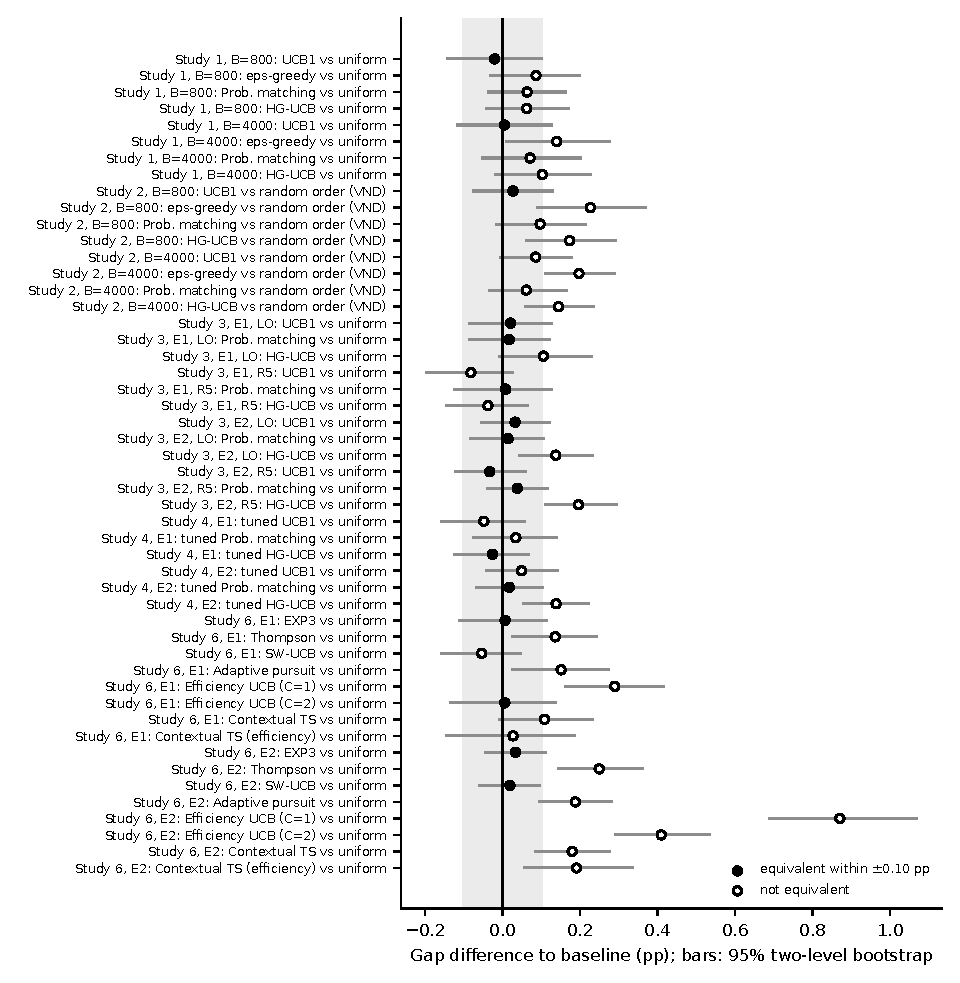
\includegraphics[width=0.9\linewidth]{fig_forest.pdf}
\caption{Equivalence audit: gap difference between each adaptive policy and its baseline in Studies 1--4 and 6. Filled markers: 90\% interval inside $\pm0.10$~pp (equivalent). Bars: 95\% two-level bootstrap intervals.}\label{fig:forest}
\end{figure}

\subsection{Reference ceiling and context}\label{sec:ceiling}
For context, HGS-CVRP \citep{vidal2022}, given the same wall-clock budget as our VNS (\num{hgs_matched_t_min}--\num{hgs_matched_t_max}~s per instance), reaches a mean gap of \num{hgs_matched}\% on the 74 instances, and \num{hgs_n01}\% with 0.1~s per customer, against \num{vns_gap_min}--\num{vns_gap_max}\% for the (non-literal) VNS variants studied here. Part of this distance is implementation language (C++ against Python), so we claim no ranking, only that no variant studied is competitive with the state of the art. An attention-based constructive model \citep{kool2019} used zero-shot reaches a mean gap of \num{kool_gap}\% over the 74 instances when the route-count constraint is ignored (\num{kool_gap_strict}\% on the \num{kool_nstrict} instances that satisfy it).
\subsection{Study 15: prospective test of the dead-weight rule}\label{sec:s15}
The full result is Table~5 and the last paragraph of Section~\mref{sec:r7} of the manuscript. The rule predicted correctly \num{s15_nok} of the \num{s15_ncel} new pool--problem cells (exact binomial $p=\num{s15_binomp}$); hypotheses H74--H76 were not confirmed and H77--H78 were (Table~\stab{tab:hip}). The primary contrasts of every cell and the contrasts against the fixed-order descent of the same pool are in the repository (\texttt{analise\_etapa15\_prim.csv}, \texttt{analise\_etapa15\_foc.csv}); the gaps of uniform selection and of the efficiency UCB in the primary sets were, in the TSP, \num{s15_gap_t5_U}\% and \num{s15_gap_t5_eff}\% (P5), \num{s15_gap_t8_U}\% and \num{s15_gap_t8_eff}\% (P8), and with time windows \num{s15_gap_w5_U}\% and \num{s15_gap_w5_eff}\% (P5), \num{s15_gap_w8_U}\% and \num{s15_gap_w8_eff}\% (P8).


\bibliographystyle{elsarticle-harv}
\bibliography{../refs}

\end{document}
